\documentclass[11pt, a4paper, titlepage]{article}
\usepackage{epsfig}
\usepackage{color}
\usepackage{amssymb}
\usepackage{amsmath}
\setlength\arraycolsep{2pt}
\setlength\tabcolsep{5pt}
\begin{document}
%%\documentclass[11pt, a4paper]{article}
%\begin{document}
\thispagestyle{empty}
\begin{center}
 \Large{\bf Changelog from Initial Submission to Final\footnote{To aid examiners only, please discard this section before final submission.}}
\end{center}
\texttt{
\tiny
\begin{enumerate}
\item[-] Removed section 7, updated rest of text accordingly.
\item[-] Rearranged section 6.4.3 and upgraded to a full section entitled `A Toy Model' to show that this standard model treatment
	 has major problems before starting. Also change the goals in section 1.5 to reflect my stance with this model.
\item[-] Section 6.5.1 reworded in order to point to the need of a central object and the problem this poses to the fermion ball scenario.
\item[-] Section 9 removed text on new technique.
\item[-] Section 1.1 removed incorrect `discrepancy with theory' sentence.
\item[-] Section 1.2 removed sentence entirely.
\item[-] Figure 5 changed IR to FIR, removed data point. Also in Figures 29-31.
\item[-] Section 1.2 added extra reference to Fermion ball studies.
\item[-] Added reference in Figure 7 at request.
\item[-] Unable to add units to Figure 12 as this is directly from astro-ph/0106209.
\item[-] Section 5.2 changes, but refuse to amend typo to `afterward' (sic)
	 as that is an Americanism. `Afterwards' is the preferred correction :D.
\item[-] Corrections to 5.3 not added as 5.4 points out clearly that the fermion ball scenario does not
	 provide an obvious minimum to the $\chi^2$. This can also be seen from figures 15, 17 and 19 being
	 almost entirely blue, meaning a good fit for either of the 2 parameters. Tables 1-3 cannot
	 possibly contain all the information of these plots. Added a sentence of this effect to 5.3.2.
	 Changed wording of 5.4.
\item[-] Section 6.1 Km/s to km/s
\item[-] Section 6.5 amended standard theory conclusions.
\item[-] References made more self-consistent.
\item[-] Section 5.1 added word `general' to not discount the incredibly rare possibility of closed 1D `harmonic oscillator'
	 solutions and emphasised the precession as the main distinguishing feature.
\item[-] Section 5.2 added clarity to comment about movement of Sgr A*.
\item[-] Section 6.1 added `cluster of stars' at request.
\item[-] Changed abstract to mention that Sgr A* does not meet the requirements for the standard model.
	 Emphasised the word simple and added a note about ADAF models.
\item[-] Section 1.2 grammar.
\item[-] Figure 2 added label and zoomed in.
\item[-] Figure 4 added extra information.
\item[-] Section 1.3 grammar.
\item[-] Equation 2 fixed typo.
\item[-] Section 5.3.1 reworded.
\item[-] Section 6.1 reworded.
\item[-] Section 6.2 fixed typo.
\item[-] Section 6.3 fixed typo.
\item[-] Section 6.5.2 more problems highlighted.
\item[-] Appendix B fixed.
\item[-] Moved Feynman diagram to section 7.
\item[-] Added a preface entitled "A Pinch of Salt".
\end{enumerate}
}
\clearpage
%\end{document}

\pagenumbering{roman}
\title{The Motion of Stars and the Accretion of Matter in the Fermion Ball and Black Hole Scenarios of the Galactic Centre}
\author{Samuel James Alexander Halliday}
\date{July, 2002}
\maketitle
%\thispagestyle{empty}
\begin{center}
 \Large{\bf A Pinch of Salt}
\end{center}
Shorty after this thesis was submitted, a paper\footnote{Sch\"{o}edel {\it et al.}, {\it Nature} {\bf 419} (2002) 694} was released
revealing shocking new results for the orbit of S0-2 around Sgr A*.
The result was an unexpectedly soon `turn' in the orbit which cannot be explained by the fermion ball scenario studied in this thesis.
As this information would
obviously require a complete rewrite of a (now) worthless thesis, it was decided best to leave the final submission in its original state,
blissfully unaware of this new data. The disproof of the fermion ball scenario is best described in this version of
Figure \ref{fig_so2bestfitssky}.
\begin{figure}[!h]
	\begin{center}
	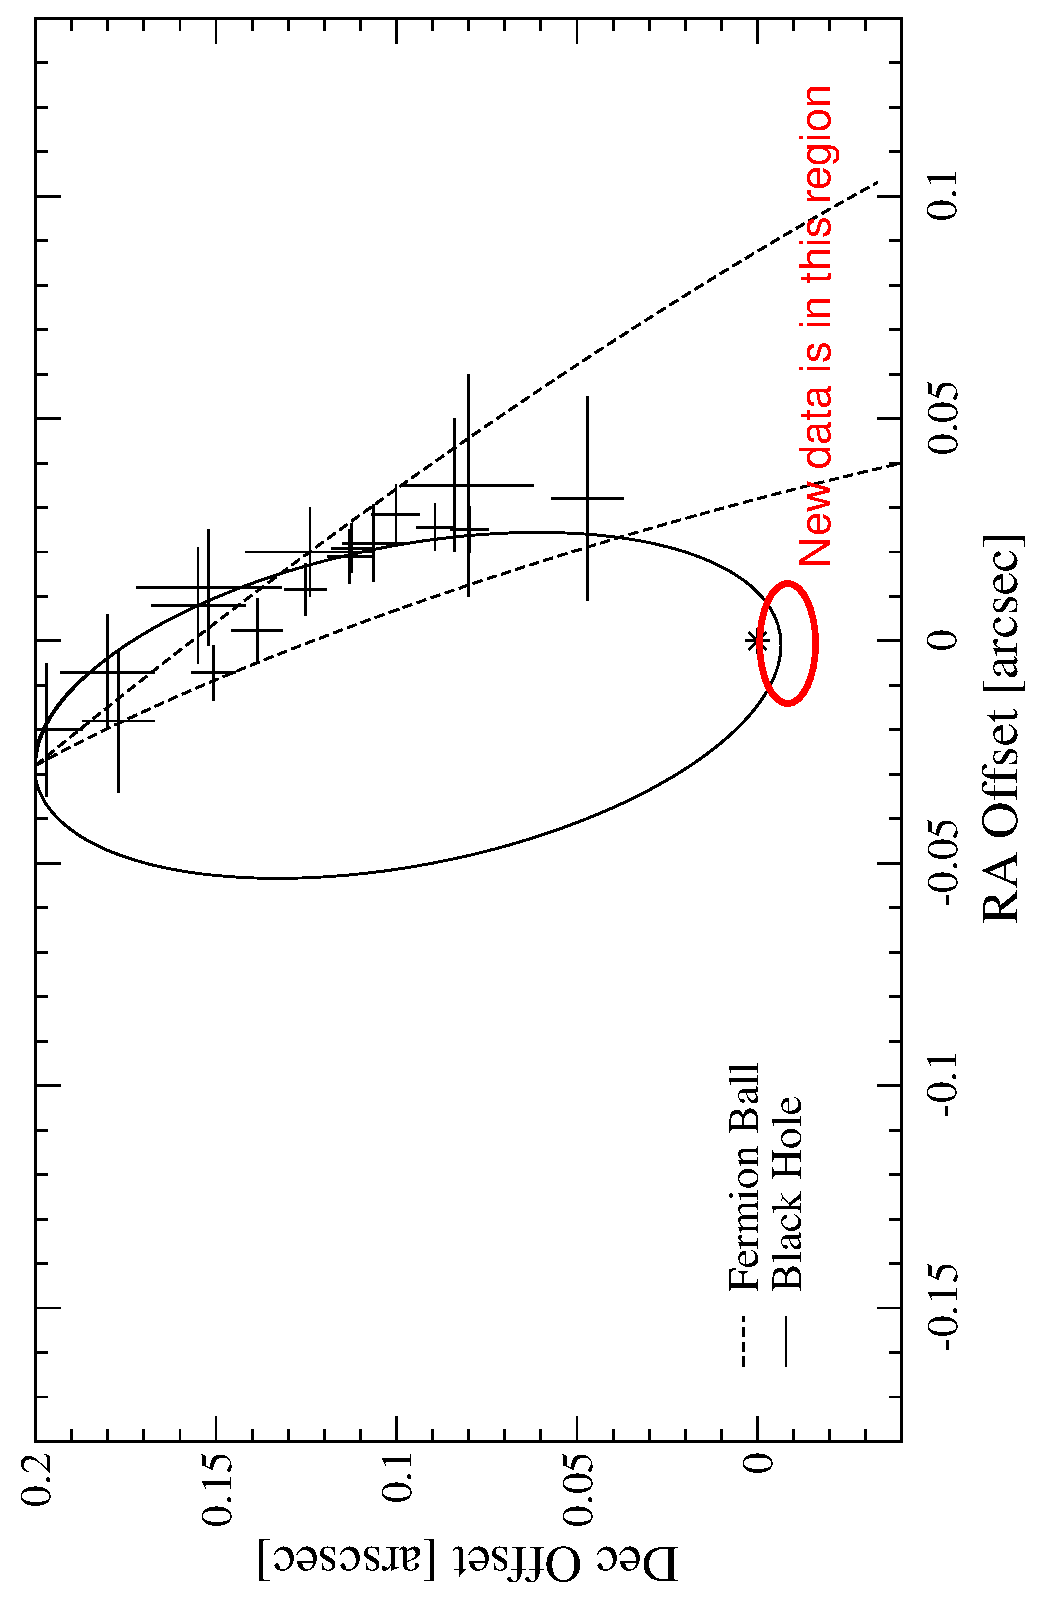
\includegraphics[angle=-90,width=0.9\textwidth]{eps/killer.eps}
	\end{center}
\end{figure}

It is clear that a black hole scenario can account for this new data (albeit with a higher than desired $\chi^2$ value using only
pre-2002 data), but that even the extremal motions for a fermion ball scenario cannot; showing that the fermion ball scenario does
not apply to the centre of our galaxy, and furthering the evidence for a black hole at the centre of the Milky Way.
\clearpage

\begin{abstract}
The motion of stars S0-1, S0-2 and S0-4, in the vicinity of the galactic centre,
is investigated using a $\chi^2$ analysis of the parameters in our line of sight.
The resulting phase spaces for the black hole and fermion ball scenarios are compared.
We find that due to the lack of accurate $z$ or $v_z$ data, the upper limit of required observational
time to discriminate between the scenarios is of the order 30 to 40 years.
Such $z$ and $v_z$ data might allow us to eliminate one of the scenarios immediately.

The spectrum from the Sgr A* region is also investigated using a {\it simple} Newtonian, optically thick
and geometrically thin model for each
scenario. As has already been known for some time, this technique is not applicable to a possible
black hole scenario at Sgr A* and as a consequence, is incapable of explaining a cut-off in the
spectrum at around $10^{13}$Hz. This cut-off follows naturally from the fermion ball potential
distribution in this simple model. It should be noted that Advection Dominated Accretion Flow models (not
investigated here) are able to predict the observed spectrum for the black hole scenario.
\end{abstract}

\tableofcontents
\clearpage
\pagenumbering{arabic}
\chapter{Introduction}
\label{intro}
\section{Noncommutative Geometry}
The formulation of quantum mechanics by Dirac \cite{Dirac} sets the
commutativity of position operators by borrowing from classical mechanics, such
that position operators commute with each other. However, this choice was merely
convenience as there was no experimental evidence to question such a definition.
It was not long before esteemed authors wrote about the effect of introducing
noncommuting coordinates \cite{Snyder:1946qz}. The motivation for studying
noncommutative geometry was to hopefully find a fix for the infinities
appearing in quantum field theory, but was sidelined as renormalisation became
successful at achieving that goal.

Noncommutative geometry has seen recent interest since open string models have
been shown to possess a noncommutative geometry \cite{witten, SW1} where there
is a non-zero $B$-field. Should string theory turn out to be a viable
explanation of our universe, one would expect to be able to observe the
noncommutativity on a quantum mechanical level. The coordinates would possess
commutator brackets of the form
\begin{equation}
  \label{eq:i:com}
  [\hat x^i, \hat x^j]=i\Theta^{ij}(\hat x)
\end{equation}
where $\Theta$ is an antisymmetric matrix. However, no such noncommutativity has
been experimentally observed \cite{Hinchliffe:2002km}. The noncommutativity
between position and momenta gives rise to the Heisenberg Uncertainty Principle
and similarly \eqref{eq:i:com} implies an uncertainty on the coordinates
themselves
\begin{equation}
  \label{eq:i:planck}
  \Delta x^i  \Delta x^j \geq \frac 12|\Theta^{ij}|
\end{equation}
This means there is no longer an idea of ``a point'', but we instead have the
notion of ``Planck cells''. The most widely studied type of noncommutative
geometry is the canonical case where $\Theta$ is a constant antisymmetric
matrix.

Unfortunately a noncommutative geometry will lead to a breaking of Lorentz
invariance. Lorentz covariance of $\Theta$ means that different inertial
observers see different noncommutativity of coordinates due to different
projections of the noncommuting planes. This is perhaps one of the greatest
hurdles for theories which rely upon a noncommutative geometry, but there is
hope. Theories such as those on $\kappa$-Minkowski spacetime
\cite{Dimitrijevic:2003wv} preserve Lorentz symmetries as deformed quantum
symmetries (a bonus from having a quantum algebra) and twisted symmetries even
for constant $\Theta$ can realise Lorentz invariance by acting in a twisted way
\cite{CKNT1, CPT1}.

A spacetime which is of particular interest is the Nappi-Witten background
\cite{NW1} which possesses a quantum algebra, is four dimensional with Minkowski
signature and is an exactly solvable background for string theory. We shall look
at the properties of this spacetime in Section \ref{sec:i:nw} and proceed to
investigate it in detail throughout this thesis.

Instead of calculating physics on a noncommutative space itself, we may
equivalently stay in commutative space and replace pointwise multiplication by a
deformed $\star$-product. A $\star$-commutator bracket between the coordinate
functions produces the functional equivalent of \eqref{eq:i:com}
\begin{equation}
  \label{eq:i:starcom}
  [ x^i,  x^j]_\star = x^i\star x^j - x^j\star x^i = i \Theta^{ij}(x)
\end{equation}
Although we shall only return to the complicated $\star$-product in detail for
Chapter \ref{star}, a basic understanding shall be assumed in Chapter
\ref{liebranes} whereby the reader recognises that in general $f\star g \neq
g\star f$ for functions depending upon the coordinates and that the
$\star$-product is not unique for a given algebra.

\section{pp-Waves and the AdS/CFT Correspondence}
A pp-wave spacetime is any Lorentzian manifold whose metric can be described in
Brinkman coordinates \cite{Brink1} as
\begin{equation}
  \label{eq:brinkman}
  G = 2dx^+dx^- + |d\mz|^2 + H(x^+, x^-, \mz)\left( d x^+\right)^2
\end{equation}
where $H(x^+, x^-, \mz)$ is any smooth function. $x^+$ is a time-like
coordinate\footnote{Please note that this convention has not been standardised
  in the literature; some authors label the time-like coordinate by $x^-$.},
$x^-$ is null and the $\mz$ are euclidean coordinates. The term ``pp'' modestly
stands for \textit{plane-fronted waves with parallel propagation}. As we shall
see in Chapter \ref{pglimits}, Penrose \cite{Penrose1} observed that near a null
geodesic, every Lorentzian spacetime looks like a plane wave. pp-waves are an
important family of exact solutions to Einstein's field equations and exhibit
the characteristic effect of a gravitational wave on light.

The AdS/CFT correspondence \cite{Aharony:1999ti} is the equivalence between a
string or supergravity theory defined on anti de Sitter space and a conformal
field theory defined on its conformal boundary, with dimension one lower. It is
the most successfully tested realisation of the holographic principle
\cite{Bousso:2002ju}.

The dynamics of strings in the backgrounds of pp-waves has been of interest
recently for a variety of reasons. They provide explicit realisations of string
theory in time-dependent backgrounds which is necessary for applications of
string cosmology. They also provide scenarios in which the AdS/CFT
correspondence may be tested beyond the supergravity approximation by taking the
Penrose limit of an $\AdS_m\times\S^n$ background \cite{BFP1} and the BMN limit
of the dual superconformal field theory \cite{BMN1}. The property of these
backgrounds that make them appealing in these contexts is that string dynamics
on them are solvable in some instances, even in the presence of non-trivial
$B$-fields \cite{BMN1,BOLPT1,Met1,PRT1,RT1}. The spectrum of the theory can be
studied in light-cone gauge wherein the two-dimensional $\sigma$-models become
free, while scattering amplitudes can be analysed using light-cone string field
theory.

D-branes (the D standing for Dirichlet) are membrane-like structures which are
considered to be as physically fundamental to string theory as the strings
themselves; they are the surfaces to which the strings are attached. If it were
not for D-branes, energy could flow along a string, slip off the endpoint and
vanish. Because the endpoints of open strings cannot detach from the D-branes to
which they are affixed, the D-branes determine the boundary conditions for the
string's equation of motion (either Neumann or Dirichlet), thereby ensuring
conservation of energy. D-branes are typically classified by their spatial
worldvolume dimension, which is indicated by a number written after the D. For
example, A D0-brane is a ``D-particle'', a D1-brane is a line (sometimes called
a ``D-string'') and a D2-brane is a plane. A ``D-instanton'' is a fixed point in
all space-time coordinates,

When D-branes are added to such closed string backgrounds, in some cases
decoupling limits exist in which one can freeze out massive open string modes
and closed string excitations. The low-energy effective theory governing the
dynamics of open strings living on the branes is non-gravitational and can be
reformulated as a field theory. The typical result is a noncommutative gauge
theory with a spacetime dependent noncommutativity parameter
\cite{CLO1,DRRS1,DN1,HS1,HT1,LNR1}. The role of spacetime dependence in these
worldvolume field theories leads to interesting violations of energy-momentum
conservation \cite{BG1,RS1}, and their potential time-dependence is especially
important for cosmological applications. In some instances the decoupled open
strings also have a dual description in terms of a gravitational theory via the
AdS/CFT correspondence \cite{HS1}. This suggests that the holographic
description of cosmological spacetimes may be described by non-local field
theories.

The general construction and analysis of noncommutative gauge theories on curved
spacetimes is one of the most important outstanding problems in the applications
of noncommutative geometry to string theory. These non-local field theories
arise naturally as certain decoupling limits of open string dynamics on D-branes
in curved superstring backgrounds in the presence of a non-constant background
Neveu-Schwarz $B$-field. On a generic Poisson manifold $M$, they are formulated
using the Kontesevich star-product \cite{Kont1} which is linked to a topological
string theory known as the Poisson sigma-model \cite{CattFel1}. Under suitable
conditions, the quantisation of D-branes in the Poisson sigma-model which wrap
coisotropic submanifolds of $M$, i.e. worldvolumes defined by first-class
constraints, may be consistently carried out and related to the deformation
quantisation in the induced Poisson bracket \cite{CattFel2}. Branes defined by
second-class constraints may also be treated by quantising Dirac brackets on the
worldvolumes \cite{CFal1}.

However, in other concrete string theory settings, most studies of
noncommutative gauge theories on curved D-branes have been carried out only
within the context of the AdS/CFT correspondence by constructing the branes as
solutions in the dual supergravity description of the gauge theory (see for
example \cite{Cai1,CLO1,HS1,HashTh1,ASY1}). It is important to understand
how to describe the classical solutions and quantisation of these models
directly at the field theoretic level in order to better understand to what
extent the noncommutative field theories capture the non-local aspects of string
theory and quantum gravity, and also to be able to extend the descriptions to
more general situations which are not covered by the AdS/CFT correspondence.

Open string dynamics on the $\NW$ background are particularly interesting
because it has the potential to display a time-dependent noncommutative geometry
\cite{DN1,HS1}, and hence the noncommutative field theories built on $\NW_6$ can
serve as interesting toy models for string cosmology which can be treated for
the most part as ordinary field theories. However, this point is rather subtle
for the present geometry \cite{DN1,HT1}. A particular gauge choice which leads
to a time-dependent noncommutativity parameter breaks conformal invariance of
the worldsheet sigma-model, i.e. it does not satisfy the Born-Infeld field
equations, while a conformally invariant background yields a non-constant but
time-independent noncommutativity. In this thesis we partially clarify this
issue.

\section{Nappi-Witten Spacetime}
\label{sec:i:nw}

In this thesis, which is based on the publications \cite{Halliday:2005zt,
  Halliday:2006qc}, we will study the noncommutative gauge theories that reside
on some D-branes in the four-dimensional Nappi-Witten gravitational wave
\cite{NW1} and its six-dimensional generalisation \cite{KM1}. We will refer to
both of these pp-waves as Nappi-Witten spacetimes and denote them respectively
by $\NW_4$ and $\NW_6$. In the full superstring setting the backgrounds we study
are $\NW_4\times\Torus^6$ and $\NW_6\times\Torus^4$, although we shall not write
the toroidal factors explicitly in what follows. We will only consider the
noncommutative deformations of the bosonic parts of these string theories, and
hence only a non-trivial NS background.

The interest in this particular class of pp-waves is that string theory in these
backgrounds can be solved completely and in a fully covariant way
\cite{BAKZ1,CFS1,DAK1,FHHP1,KK1,KKL1,RT2}. They describe homogeneous
gravitational waves (Hpp-waves) and represent the ``minimal'' deformation of
flat spacetime by $H$-flux ($H=dB$, the flux associated to the NS field). They
may be formulated as WZW models based on a twisted Heisenberg group, for which
the wave is an exact solution of the worldsheet $\sigma$-model \cite{KM1,NW1}.

The $\NW_6$ spacetime already captures the generic features of
higher-dimensional Hpp-waves. It can be regarded as the Penrose-G\"uven limit of
the background $\AdS_3\times$ $\S^3\times\Torus^4$ \cite{BFP1,BFHP1} supported
by an NS--NS three-form flux, which describes the near horizon geometry of an
NS5/F1 bound state \cite{GKS1}. The dual superconformal field theory is believed
to be the nonlinear $\sigma$-model with target space the symmetric product
orbifold ${\rm Sym}^N(\Torus^4)$. Similarly, the plane wave metric of $\NW_4$
arises from the Penrose limit of $\AdS_2\times\S^2$ \cite{BFP1,BFHP1}.

Both $\NW_4$ and the Penrose limit of $\AdS_3\times\S^3$ are examples of
non-dilatonic, pp-wave solutions of six-dimensional supergravity \cite{SS-J1}.
However, as we later discuss in detail, the Penrose-G\"uven limit of
$\AdS_2\times\S^2$ does {\it not} induce the full NS-supported geometry of the
$\NW_4$ spacetime. Therefore, contrary to some claims \cite{DeKa1,SF1}, the
four-dimensional Nappi-Witten spacetime cannot be studied as the Penrose-G\"uven
limit of $\AdS_2\times\S^2$. Instead, it arises as a Penrose-G\"uven limit of
the near horizon geometry of NS5-branes \cite{GO1}, on which string theory is
dual to little string theory. This feature can be understood by regarding
$\AdS_2\times\S^2$ as the worldvolume of a symmetric D-brane in the
$\AdS_3\times\S^3$ spacetime, while $\NW_4$ may only be realised as the
worldvolume of a non-symmetric D-brane in $\NW_6$.

We shall find that the most natural plane wave limits of embedded
$\AdS_2\times\S^2$ submanifolds of $\AdS_3\times\S^3$ correspond to two classes
of symmetric D-branes in $\NW_6$. The first one is a {\it flat} euclidean
D3-brane in a constant magnetic field, which carries a noncommutative
worldvolume field theory with constant noncommutativity parameter determined by
the constant time slices of the plane wave background. The second one is a
Lorentzian D3-brane isometric to $\NW_4$ with vanishing NS fields but with a
null worldvolume electric field, which is described in the decoupling limit by a
non-gravitational theory of noncommutative open strings, rather than by a
noncommutative field theory. It is tempting to speculate that the full $\NW_4$
deformation of this noncommutative open string theory describes the dynamics of
the dual little string theory.

This problem is not peculiar to the class of plane wave geometries that we
study, and it leads us into a detailed investigation of how D-branes behave
under the Penrose-G\"uven limit of a spacetime. Similar analyses in some
specific contexts are considered in \cite{DK2,SZ1,SF1}. We formulate and solve
this problem in some generality, and then apply it to our specific backgrounds
of interest. With this motivation at hand, we then proceed to reanalyse the
classification of the symmetric D-branes of $\NW_6$, elaborating on the analysis
initiated in \cite{FS1,SF1} and extending it to a detailed study of the
worldvolume supergravity fields supported by each of these branes.

We also clarify some points which were missed in the analysis of \cite{SF1}. In
each instance we identify the $\AdS_3\times\S^3$ origin of the brane in
question, and quantise its worldvolume geometry using standard techniques and
the representation theory of the twisted Heisenberg group
\cite{BAKZ1,CFS1,KK1,Streater1}. We will find that most of these branes support
{\it local} worldvolume effective field theories, because on most of them the
pertinent supergravity form fields are trivial. In fact, we find that all
symmetric D-branes in $\NW_6$ (both twisted and untwisted) have vanishing NS--NS
three-form flux, and only the two classes of branes mentioned above support a
non-vanishing gauge-invariant two-form field. The overall consistency of these
results, along with their agreement with the exact boundary conformal field
theory description of Cardy branes in $\NW_4$ \cite{DK2}, provides an important
check that the standard techniques for quantisation of worldvolume geometries in
compact group manifolds (see \cite{Schom1} for a review) extend to these classes
of non-compact (and non-semisimple) Lie groups.

Somewhat surprisingly, even the spacetime filling symmetric D5-brane in $\NW_6$
has trivial supergravity form fields. Motivated by this fact, we systematically
construct the noncommutative geometry underlying the non-local field theory
living on a non-symmetric D5-brane wrapping $\NW_6$. The resulting
noncommutativity is non-constant, but independent of the plane wave time
coordinate. This agrees with the recent analysis in \cite{HT1} of the
Dolan-Nappi model \cite{DN1} which describes a time-dependent noncommutative
geometry on the worldvolume of a D3-brane wrapping $\NW_4$. However, the
background used in \cite{DN1} is not conformally invariant and hence not a
closed string background. Correctly reinstating conformal invariance \cite{HT1}
gives a spatially dependent but time-independent noncommutativity parameter. We
elaborate on this noncommutativity somewhat and show that it may be regarded as
arising from a formal quantisation of the twisted Heisenberg algebra.

In Section \ref{NWPW} we review the definition and geometrical properties of the
four-dimensional Nappi-Witten spacetime. We show that its natural pp-wave
isometry group is isomorphic to the six-dimensional twisted Heisenberg group,
paving the way to an analysis of the isometric embeddings
$\NW_4 \hookrightarrow \NW_6$. We also emphasise the time-independent harmonic
oscillator character of point-particle dynamics in these backgrounds, as it
helps to clarify the nature of the noncommutative worldvolume field theories
constructed later on. In Section \ref{IsomEmb} we study the interplay between
isometric embeddings and Penrose-G\"uven limits of branes, first in generality
and then to the particular instances of Nappi-Witten spacetimes. From this
analysis it becomes clear that both the $\NW_4$ and $\NW_6$ gravitational waves
are necessarily wrapped by non-symmetric D-branes. In Section \ref{NCBranes} we
begin our analysis of the symmetric branes in $\NW_6$, beginning with those
described by conjugacy classes of the twisted Heisenberg group.

We identify classes of null branes (with degenerate worldvolume metrics), and
show that their quantised geometries are commutative but generically differ from
those of the classical conjugacy classes due to a unitary rotational symmetry of
the background. We also find a class of euclidean D3-branes and show, directly
from the representation theory of the twisted Heisenberg group, that their
worldvolumes carry a Moyal-type noncommutativity akin to that induced on branes
in constant magnetic fields \cite{DNek1,SW1,Sz1,Sz2}. This sort of
noncommutativity is natural from the point of view of the time-independent
harmonic oscillator dynamics. In Section \ref{TwistedNCBranes} we analyse
symmetric branes in $\NW_6$ which are described by twisted conjugacy classes. We
show, again through explicit quantisation via representation theory and analysis
of the worldvolume supergravity fields, that the low-energy effective field
theories on {\it all} twisted D-branes are local.

\subsection{Definitions}
\label{NWPW}
In this section we will define and analyse the geometry of the Nappi-Witten
spacetime $\NW_4$ \cite{NW1}. It is a four-dimensional homogeneous spacetime of
Minkowski signature which defines a monochromatic plane wave. It is further
equipped with a supergravity NS $B$-field of constant flux, which in the
presence of D-branes is responsible for the spacetime noncommutativity of the
pp-wave. We will emphasise the simple, time-independent harmonic oscillator form
of the dynamics in this background, as it will play a crucial role in subsequent
sections.

The spacetime $\NW_4$ is defined as the group manifold of the Nappi-Witten
group, the universal central extension of the two-dimensional euclidean group
${\rm ISO}(2)={\rm SO}(2)\ltimes\R^2$. The corresponding simply connected
group $\mathcal N_4$ is homeomorphic to four-dimensional Minkowski space
$\E^{1,3}$. Its non-semisimple Lie algebra $\mathfrak n_4$ is generated by
elements $\P^\pm$, $\J$, $\T$ obeying the commutation relations
\begin{eqnarray}
  \label{NW4algdef}
  \left[\P^+ , \P^-\right]&=&2 i \T \nn\\
  \left[\J , \P^\pm\right]&=&\pm i \P^\pm \nn\\
  \left[\T , \J\right]&=&\left[\T , \P^\pm\right] = 0
\end{eqnarray}
This is just the three-dimensional Heisenberg algebra extended by an outer
automorphism which rotates the noncommuting coordinates. The twisted Heisenberg
algebra may be regarded as defining the harmonic oscillator algebra of a
particle moving in one-dimension, with the additional generator $\J$ playing the
role of the number operator (or equivalently the oscillator hamiltonian). It is
a solvable algebra whose properties are much more tractable than, for instance,
those of the ${\rm su}(2)$ or ${\rm sl}(2,\R)$ Lie algebras which are at the
opposite extreme.

The centre of the universal enveloping algebra $U(\mathfrak n_4)$ contains the
central element $\T$ of the Lie algebra $\mathfrak{n}_4$ and also the quadratic
Casimir element
\begin{equation}
  \label{NW4Casimir}
  \Casimir_4=2 \J \T+ \frac12 \left(\P^+ \P^-+\P^- \P^+\right)
\end{equation}
The most general invariant, non-degenerate symmetric bilinear form $\langle
\cdot , \cdot \rangle:\mathfrak{n}_4\times\mathfrak{n}_4\to\R$ is defined by
\cite{NW1}
\begin{eqnarray}
  \label{NW4innerprod}
  \left\langle\P^+ , \P^-\right\rangle&=&2 
  \left\langle\J , \T\right\rangle = 2 \nn\\
  \left\langle\J , \J\right\rangle&=&b \nn\\
  \left\langle\P^\pm , \P^\pm\right\rangle&=&
  \left\langle\T , \T\right\rangle = 0 \nn\\
  \left\langle\J , \P^\pm\right\rangle&=&\left\langle\T , 
    \P^\pm\right\rangle = 0
\end{eqnarray}
for any $b\in\R$. This inner product has Minkowski signature (when $b=0$), so
that the group manifold of $\mathcal N_4$ possesses a homogeneous, bi-invariant
Lorentzian metric defined by the pairing of the Cartan-Maurer left-invariant,
$\mathfrak n_4$-valued one-forms $g^{-1} d g$ for $g\in\mathcal N_4$ as
\begin{equation}
  \label{NW4CM}
  d s_4^2=\left\langle g^{-1}  d g , g^{-1}  d g\right\rangle
\end{equation}
A generic group element $g\in\mathcal N_4$ may be parametrised as
\begin{equation}
  \label{NW4coords}
  g(u,v,a,\overline{a} )=e^{a \P^++\overline{a} \P^-} 
  e^{\theta u \J} e^{\theta^{-1} v \T}
\end{equation}
where $u,v\in\R$, $a\in\C$, and the parameter $\theta\in\R, \theta > 0$ controls
the strength of the NS $B$-field background. In these global coordinates, the
Cartan-Maurer one-form is given by
\begin{equation}
  \label{NW4CMform}
  g^{-1}  d g=e^{- i \theta u}  d a \P^++e^{ i \theta u} 
  d\overline{a} \P^-+\theta  d u \J+\left(\theta^{-1}  d v+ i 
    a  d\overline{a}- i \overline{a}  d a\right) \T
\end{equation}
so that the metric \eqref{NW4CM} reads
\begin{equation}
  \label{NW4metricNW}
  d s_4^2=2  d u  d v+| d a|^2+2 i \theta \left(a 
    d\overline{a}-\overline{a}  d a\right)  d u+b \theta^2  d u^2
\end{equation}

The metric \eqref{NW4metricNW} assumes the standard form of the plane wave
metric for a conformally flat, indecomposable Cahen-Wallach Lorentzian symmetric
spacetime $\CW_4$ in four dimensions \cite{CW1} upon introduction of Brinkman
harmonic coordinates $(x^+,x^-,z)$ \cite{Brink1} defined by rotating the
transverse plane at a Larmor frequency as $u=x^+$, $v=x^-$ and $a=e^{\frac{ i
    \theta}2 x^+} z$. In these coordinates the metric assumes the stationary form
\begin{equation}
  \label{NW4metricBrink}
  d s_4^2=2  d x^+  d x^-+| d z|^2+\theta^2 
  \left(b-\frac14 |z|^2\right) 
  \left( d x^+\right)^2
\end{equation}
revealing the pp-wave nature of the geometry for $b=0$. The physical meaning of
the arbitrary parameter $b$ will be elucidated below. It may be set to zero by
exploiting the translational symmetry of the geometry in $x^-$ to shift $x^-\to
x^--\frac{\theta^2 b}2 x^+$, which corresponds to a Lie algebra automorphism of
$\mathfrak n_4$. Note that on the null planes of constant $u=x^+$, the geometry
becomes that of flat two-dimensional euclidean space $\E^2$. This is the
geometry appropriate to the Heisenberg subgroup of $\mathcal{N}_4$, where the
effects of the twisting generator $\J$ are turned off.

Thus far, the Nappi-Witten spacetime has been described geometrically as a
four-dimensional Cahen-Wallach space $\CW_4$. The spacetime $\NW_4$ is further
supported by a Neveu-Schwarz two-form field $B_4$ of constant field strength
\begin{equation}
  \label{NS3formBrink}
  H_4=-\frac13 \bigl\langle g^{-1}  d g , 
  \left[g^{-1}  d g , g^{-1}  d g\right]\bigl\rangle
   = 2 i \theta  d x^+\wedge d z\wedge d\overline{z} =  d B_4
\end{equation}
where
\begin{equation}
  \label{NS2formBrink}
  B_4=-\frac12 \bigl\langle g^{-1}  d g , 
  \frac{\1+{\rm Ad}_g}{\1-{\rm Ad}_g} g^{-1}  d g\bigl\rangle = 
  2 i \theta x^+  d z\wedge d\overline{z}
\end{equation}
is defined to be non-zero only on those vector fields lying in the range of the
operator $\1-{\rm Ad}_g$ on $T_g\mathcal{N}_4$, i.e. on vectors tangent to the
conjugacy class containing $g\in\mathcal{N}_4$. The corresponding contracted
two-form $H_4^2$ compensates exactly the constant Riemann curvature of the
metric \eqref{NW4metricBrink}, so that $\NW_4$ provides a viable supergravity
background. In fact, in this case the cancellation is exact at the level of the
full string equations of motion, so that the plane wave is an exact background
of string theory \cite{NW1}. It is the presence of this $B$-field that induces
noncommutativity of the string background in the presence of D-branes.

\subsection{Isometries}
\label{Isoms}
The realisation of the geometry of $\NW_4$ as a standard plane wave of
Cahen-Wallach type enables us to study its isometry group using the standard
classification \cite{BOL1}. Writing $\partial_\pm := \partial/\partial x^\pm$,
the metric \eqref{NW4metricBrink} has the obvious null Killing vector
\begin{equation}
  \label{ZKilling}
  T=\theta \partial_-
\end{equation}
generating translations in $x^-$ and characterising a pp-wave, and also the null
Killing vector
\begin{equation}
  \label{HKilling}
  J=\theta^{-1} \partial_+
\end{equation}
generating translations in $x^+$. An analysis of the Killing equations
\cite{BOL1} shows that there are also four extra Killing vectors $P^{(k)}$,
$P^{\prime (k)}$, $k=1,2$ which generate twisted translations in the transverse
plane $z\in\C$ to the motion of the plane wave. Denoting
$\partial:=\partial/\partial z$, they are given in the form
\begin{eqnarray}
  \label{XkXprimegen}
  P^{(k)}&=&c^{(k)}(x^+) \partial+\overline{c}^{ (k)}(x^+) 
  \overline{\partial}-\theta^{-1} \left(\dot c^{(k)}(x^+) \overline{z}+
    \dot{\overline{c}}^{ (k)}(x^+) z\right) \partial_- \nn\\
  P^{\prime (k)}&=&c^{\prime (k)}(x^+) \partial+\overline{c}^{ 
    \prime (k)}(x^+) 
  \overline{\partial}-\theta^{-1} \left(\dot c^{\prime (k)}(x^+) \overline{z}+
    \dot{\overline{c}}^{ \prime (k)}(x^+) z\right) \partial_-  
\end{eqnarray}
where the dots denote differentiation with respect to the light-cone time
coordinate $u=x^+$, and the complex-valued coefficient functions in
\eqref{XkXprimegen} solve the harmonic oscillator equation of motion
\begin{equation}
  \label{HODE}
  \dot c(x^+)=-\frac{\theta^2}4 c(x^+)  
\end{equation}
The four linearly independent solutions of \eqref{HODE} are characterised by
their initial conditions on the null surface $x^+=0$ as
\begin{eqnarray}
  \label{cinitialconds}
  c^{(k)}(0) = \delta_{k1}+ i \delta_{k2} && \dot c^{(k)}(0) = 0\nn\\
  c^{\prime (k)}(0) = 0 && \dot c^{\prime (k)}(0) =
  \theta \left(\delta_{k1}+ i \delta_{k2}\right)  
\end{eqnarray}

The solutions of \eqref{HODE} and \eqref{cinitialconds} are given by
\begin{eqnarray}
  \label{cexplsoln}
  c^{(1)}(x^+) = \cos\frac{\theta x^+}2 &&
  c^{(2)}(x^+) =  i \cos\frac{\theta x^+}2   \nn\\
  c^{\prime (1)}(x^+) = 2\sin\frac{\theta x^+}2 &&
  c^{\prime (2)}(x^+) = 2 i \sin\frac{\theta x^+}2  
\end{eqnarray}
An interesting feature of these functions is that they generate the Rosen form
\cite{Rosen1} of the plane wave metric \eqref{NW4metricBrink}. It is defined by
the transformation to local coordinates $(u,v,y^1,y^2)$ given by
\begin{eqnarray}
  \label{Rosen}
  u&=&x^+   \nn\\v&=&x^--\frac\theta4 (z+\overline{z} )^2 
  \tan\frac{\theta x^+}2-\frac\theta4 (z-\overline{z} )^2 
  \cot\frac{\theta x^+}2    \nn\\y^1&=&\frac12  
  \left((z+\overline{z} )\sec\frac{\theta x^+}2 + i (z-\overline{z} )
    \csc\frac{\theta x^+}2 \right)   \nn\\y^2&=&\frac12  
  \left((z+\overline{z} )\sec\frac{\theta x^+}2 - i (z-\overline{z} )
    \csc\frac{\theta x^+}2 \right)  
\end{eqnarray}
under which the metric becomes
\begin{equation}
  \label{NW4metricRosen}
  d s_4^2=2  d u  d v+C_{ij}(u)  d y^i  d y^j+b \theta^2  d u^2
\end{equation}
where
\begin{equation}
  \label{Cumatrix}
  C(u)=\bigl(C_{ij}(u)\bigr)=
  \begin{pmatrix}
    1&\cos\theta u\\\cos\theta u&1
  \end{pmatrix}  
\end{equation}
This form of the metric is degenerate at the conjugate points where $\cos\theta
u=\pm 1$. The harmonic oscillator solutions \eqref{cexplsoln} then generate an
orthonormal frame for the transverse plane metric \eqref{Cumatrix},
\begin{equation}
  \label{CQrel}
  C(u)=E(u) E^\top(u)  
\end{equation}
with
\begin{eqnarray}
  \label{Qvielbein}
  E=\frac12
  \begin{pmatrix}c^{(1)}+\frac12  c^{\prime (2)}+
    \overline{c}^{ (1)}+\frac12  \overline{c}^{ \prime
      (2)}& &-\left(c^{(2)}-\frac12  c^{\prime (1)}+
      \overline{c}^{ (2)}-\frac12  \overline{c}^{ \prime
        (1)}\right)\\c^{(1)}+\frac12  c^{\prime (2)}+
    \overline{c}^{ (1)}+\frac12  \overline{c}^{ \prime
      (2)}& &c^{(2)}-\frac12  c^{\prime (1)}+
    \overline{c}^{ (2)}-\frac12  \overline{c}^{ \prime(1)}
  \end{pmatrix}
\end{eqnarray}
satisfying the symmetry condition
\begin{equation}
  \label{Esymcond}
  \dot E(u) E^\top(u)=E(u) \dot E^\top(u)
\end{equation}
Note that in contrast to the Brinkman coordinate system, in the Rosen form
\eqref{NW4metricRosen} two extra commuting translational symmetries in the
transverse plane $(y^1,y^2)$ are manifest, while time translation symmetry is
lost.

By defining $P^\pm:=P^{\prime (1)}\pm i P^{(1)}$ and $ Q^{\pm}:=P^{\prime
  (2)}\pm i P^{(2)}$, the six Killing vectors generated by the basic
Cahen-Wallach structure of the plane wave may be summarised as
\begin{eqnarray}
  \label{6CWKilling}
  T&=&\theta \partial_-   \\
  J&=&\theta^{-1} \partial_+   \nn\\
  P^\pm&=&\left(\sin\frac{\theta x^+}2 \pm i e^{\mp 
      \frac{ i \theta}2 x^+}\right)
  \left(\partial+\overline{\partial} \right)-\theta e^{\mp 
    \frac{ i \theta}2 x^+} \left(
    z+\overline{z} \right) \partial_-   \nn\\
  Q^{\pm}&=&\left( i \sin\frac{\theta x^+}2 \mp
    e^{\mp \frac{ i \theta}2 x^+}\right)
  \left(\partial-\overline{\partial} \right)+ i \theta e^{\mp 
    \frac{ i \theta}2 x^+} \left(
    z-\overline{z} \right) \partial_-  \nn
\end{eqnarray}
Together, they generate the harmonic oscillator algebra
$\mathfrak{n}_6$ of a particle moving in {\it two} dimensions,
\begin{eqnarray}
  \label{NW4isomalg}
  \left[P^\alpha ,  Q^{\beta}\right]&=&0 \qquad\qquad\alpha,\beta=\pm   \\
  \left[T ,P^\pm\right]&=&\left[T, Q^{\pm}\right] = \left[T , J\right] = 0\nn\\
  \left[P^+ , P^-\right]&=&\left[Q^{+}, Q^{-}\right] = 2iT\nn\\
  \left[J , P^\pm\right]&=&\pm iP^\pm\nn\\
  \left[J ,  Q^{\pm}\right]&=&\pm i  Q^{\pm} \nn
\end{eqnarray}
This isometry algebra acts transitively on the null planes of constant
  $x^+$ and it generates a central extension ${\mathcal
  N}_6$ of the subgroup
\begin{equation}
  \label{S5subgp}
  \mathcal{S}_5={\rm SO}(2)\ltimes\R^4
\end{equation}
of the four-dimensional euclidean group ${\rm ISO}(4)={\rm SO}(4)\ltimes\R^4$,
where ${\rm SO}(2)$ is the diagonal subgroup of ${\rm SO}(2)\times{\rm
  SO}(2)\subset{\rm SO}(4)$. It is defined by extending the commutation
relations \eqref{NW4algdef} by generators $\Q^{\pm}$ obeying relations as in
\eqref{NW4isomalg}. The quadratic Casimir element $\Casimir_6\in
U(\mathfrak{n}_6)$ and inner product on $\mathfrak{n}_6$ are defined in the
obvious way by extending \eqref{NW4Casimir} and \eqref{NW4innerprod}
symmetrically under $\P^\pm\leftrightarrow\Q^\pm$.

Following the analysis of the previous section, one can show that the
group manifold of ${\mathcal N}_6$ is a six-dimensional Cahen-Wallach
space $\CW_6$, with Brinkman metric
\begin{equation}
  \label{NW6metricBrink}
  d s_6^2=2  d x^+  d x^-+| d\mz|^2+\theta^2\left(b-\frac14
    |\mz|^2\right)\left( d x^+\right)^2
\end{equation}
where $\mz^\top=(z,w)\in\C^2$, which carries a constant Neveu-Schwarz
three-form flux
\begin{eqnarray}
  \nn H_6&=&-2 i \theta  d x^+\wedge d\overline{\mz}^{ \top}
  \wedge d\mz= d B_6\\\label{NW6Bfield}
  B_6&=&-2 i \theta x^+  d\overline{\mz}^{ \top}\wedge d\mz  
\end{eqnarray}
It thereby defines a six-dimensional version $\NW_6$ of the Nappi-Witten pp-wave
\cite{KM1}. This observation will be exploited in the ensuing sections to view
the Nappi-Witten wave as an isometrically embedded D-submanifold ${\rm
  NW}_4\hookrightarrow{\rm NW}_6$. In this setting, it corresponds to a
symmetry-breaking D3-brane in a non-zero $H$-flux.

However, for the Nappi-Witten wave this is not the end of the story. Because of
the bi-invariance of the metric \eqref{NW4CM}, the actual isometry group is the
direct product $\mathcal N_4\times\overline{\mathcal N}_4$ acting by left and
right multiplication on the group $\mathcal N_4$ itself. Since the left and
right actions of the central generator $\T$ coincide, the isometry group is
seven-dimensional. In the present basis, the missing generator from the list
\eqref{6CWKilling} is the left-moving copy $\overline{J}$ of the oscillator
hamiltonian with
\begin{equation}
  \label{JPpm}
  \left[ \overline{J} , P^\pm\right]=\mp i 
  P^\pm+ Q^{\pm}      \left[ \overline{J} , 
    Q^{\pm}\right]=\mp i  Q^{\pm}-P^\pm  
\end{equation}
and it is straightforward to compute that it is given by
\begin{equation}
  \label{extraHKilling}
  \overline{J}=-\theta^{-1} \partial_+- i \left(z \partial-\overline{z} 
    \overline{\partial} \right)  
\end{equation}
The vector field $J+\overline{J}$ generates rigid rotations in the transverse
plane.

\subsection{Commutative Field Theory}
\label{Dynamics}
Standard covariant quantisation of a massless relativistic scalar particle in
$\NW_4$ leads to the Klein-Gordon equation in the curved background,
\begin{equation}
  \label{KGeqn}
  \Box_4\phi = 0  
\end{equation}
where
\begin{equation}
  \label{BoxNW4def}
  \Box_4=2 \partial_+ \partial_--\theta^2 
  \left(b-\frac14  |z|^2\right) \partial_-^2+|\partial|^2
\end{equation}
is the laplacian corresponding to the Brinkman metric \eqref{NW4metricBrink}. It
coincides with the Casimir \eqref{NW4Casimir} expressed in terms of left or
right isometry generators \eqref{6CWKilling}, \eqref{extraHKilling}. The
dependence on the light-cone coordinates $x^\pm$ drops out of the Klein-Gordon
equation because of the isometries generated by the Killing vectors
\eqref{ZKilling} and \eqref{HKilling}.

By using a Fourier transformation of the covariant Klein-Gordon field
$\phi$ along the $x^-$ direction,
\begin{equation}
  \label{KGphiFT}
  \phi\left(x^+,x^-,z,\overline{z} \right)=\int\limits_{-\infty}^\infty
  d p^+ \psi\left(x^+,z,\overline{z};p^+\right) e^{ i  p^+x^-}  
\end{equation}
we may write \eqref{KGeqn} equivalently as
\begin{equation}
  \label{KGmomsp}
  \left[|\partial|^2+2 i  p^+ \partial_++\left(b-
      \frac14  |z|^2\right) \left(\theta p^+\right)^2\right]\psi\left(x^+,z,
    \overline{z};p^+\right)=0  
\end{equation}
Introducing the time parameter $\tau$ through
\begin{equation}
  \label{utaudef}
  u=x^+=p^+ \tau  
\end{equation}
the differential equation \eqref{KGmomsp}) becomes the
Schr\"odinger wave equation
\begin{equation}
  \label{SchHO}
  i  \frac{\partial\psi\left(\tau,z,\overline{z};p^+\right)}{\partial\tau}=
  \left[-\frac12  |\partial|^2+\frac12  \left(
      \frac{\theta p^+}2 \right)^2 
    |z|^2-\frac b2  \left(\theta p^+\right)^2\right]\psi\left(\tau,z,
    \overline{z};p^+\right)
\end{equation}
for the non-relativistic two-dimensional harmonic oscillator with a time
independent frequency given by the light-cone momentum and $H$-flux as
$\omega=|\theta p^+|/2$. The only role of the arbitrary parameter $b$ is to shift
the zero-point energy of the harmonic oscillator, and it thereby carries no
physical significance.

Let us remark that the same hamiltonian that appears in the Schr\"odinger
equation \eqref{SchHO} could also have been derived in light-cone gauge in the
plane wave metric \eqref{NW4metricBrink} starting from the massless relativistic
particle Lagrangian
\begin{equation}
  \label{masslessLag}
  L=\dot x^+ \dot x^-+\frac{\theta^2}2  \left(b-\frac14  
    |z|^2\right) \left(\dot x^+\right)^2+\frac12  \left|\dot z\right|^2
\end{equation}
describing free geodesic motion in the Nappi-Witten spacetime. In the light-cone
gauge, the light-cone momentum is $p^+=p_-=\partial L/\partial\dot x^-=\dot
x^+=1$, while the hamiltonian is $J=p_+=\partial L/\partial\dot x^+$. Imposing
the mass-shell constraint $L=0$ at $\dot x^+=1$ gives the equation of motion for
$x^-$, which when substituted into $J$ yields exactly the hamiltonian appearing
on the right-hand side of \eqref{SchHO} with transverse momentum $p^{
}_\perp=\dot z=- i \partial$.

The time-independence of the effective dynamics here follows from homogeneity of
the plane wave geometry, which prevents dispersion along the light-cone time
direction. These calculations give the quantisation of a particle in $\NW_4$
only in the commutative geometry limit, i.e. in the spacetime $\CW_4$, because
they do not incorporate the supergravity $B$-field supported by the Nappi-Witten
spacetime. In the following we will describe how to incorporate the deformation
of $\CW_4$ caused by the non-trivial NS-sector. Henceforth we will drop the
zero-point energy and set $b=0$.

\subsection{Isometric Embeddings of Branes}
\label{IsomEmb}
A remarkable feature of the Nappi-Witten spacetime is the extent to which it
shares common features with many of the more ``standard'' curved spaces. It is
formally similar to the spacetimes built on the ${\rm SL}(2,\R)$ and ${\rm
  SU}(2)$ group manifolds, but in many ways is much simpler. As a twisted
Heisenberg group, it lies somewhere in between these curved spaces and the flat
space based on the usual Heisenberg algebra. One way to see this feature at a
quantitative level is by examining Penrose-G\"uven limits involving the
(universal covers of the) ${\rm SL}(2,\R)$ and ${\rm SU}(2)$ group manifolds
which produce the spacetime $\NW_4$. This will provide an aid in understanding
various physical properties which arise in later constructions.

In looking for D-submanifolds, we are primarily interested in D-embeddings which
are NS-supported and thereby carry a noncommutative geometry. As we will
discuss, this involves certain important subtleties that must be carefully taken
into account. As the Nappi-Witten spacetime can be viewed as a Cahen-Wallach
space, i.e. as a plane wave, its geometry will arise as Penrose limits of other
metrics. This opens up the possibility of extracting features of $\NW_4$ by
mapping them directly from properties of simpler, better studied noncommutative
spaces. In this section we will begin with a thorough general analysis of the
interplay between Penrose-G\"uven limits and isometric embeddings of Lorentzian
manifolds, and derive simple criteria for the limit and embedding to commute.
Then we apply these results to derive the possible limits that can be used to
describe the NS-supported D-embeddings of $\NW_4$.

\section{Outline of Thesis}
The outline of this thesis is as follows. In Chapter \ref{pglimits} we introduce
the concept of the Penrose-G\"{u}ven limit and impose a constraint for isometric
embedding diagrams. We then examine the Lie branes of $\NW_6$ in Chapter
\ref{liebranes}, highlighting the implied noncommutative geometries. We close
the Chapter with the discovery of a time dependent, noncommutative geometry on
$\NW_6$ which exhibits the same algebra as $\mathfrak{n}_6$.

The discovery of such a spacetime is motivation for studying three classes of
Nappi-Witten $\star$-products in Chapter \ref{star}. We construct the necessary
tools for investigating the associated free scalar field theories and Chapter
\ref{fieldtheory} concludes by investigating the field theories of our three
orderings and the regularly embedded D-branes in $\NW_6$.

%%% Local Variables: 
%%% mode: latex
%%% TeX-master: "main.tex"
%%% End: 

\section{Non-Relativistic Mass Distribution}
\label{sec_classical}
\begin{quotation}
	\raggedleft \it I know that this defies the law of gravity, \\ but, you see, I never studied law. \\ -- Bugs Bunny
\end{quotation}
In order to obtain the mass distribution of the fermion ball, let us first look at a simple Newtonian model 
\cite{ref_classicalapproach}, in which the gravitational potential satisfies Poisson's equation
\begin{equation}
	\nabla \Phi(r) = -4 \pi G \rho_{\nu}(r)
	\label{eqn_poisson}
\end{equation}
where $G$ is Newton's gravitational constant and $\rho_{\nu}(r)$ the mass density of the fermions and anti-fermions at a
particular radius $r$. The self-gravity of the fermionic matter may be balanced with its degeneracy pressure, obeying the
equation of hydrostatic equilibrium
\begin{equation}
	\frac{1}{\rho_{\nu}} \frac{dP_{\nu}}{dr} + \frac{d\Phi}{dr} = 0
	\label{eqn_hydroequil}
\end{equation}
Here the pressure is given by the polytropic equation of state for non-relativistic fermionic matter at zero temperature.
\begin{equation}
	P_{\nu} = K \rho_{\nu}^{\frac{5}{3}}
	\label{eqn_polytropic}
\end{equation}
with the constant $K$ given by \cite{ref_thomasfermiapproach}
\begin{equation}
	K = \left(\frac{6}{g_{\nu}}\right)^{\frac{2}{3}} \frac{\pi^{\frac{4}{3}} \hbar^2}{5 m_{\nu}^{\frac{8}{3}}}
	\label{eqn_polytropicconstant}
\end{equation}
where $g_{\nu}$ represents the number of degrees of freedom of the fermions (spin and particle-antiparticle degeneracy),
either 2 (Majorana) or 4 (Dirac), $m_{\nu}$ being the fermion rest mass. We thus obtain
\begin{equation}
	\frac{5}{2} K \rho^{\frac{2}{3}} + \Phi = E_0
	\label{eqn_classicalarb1}
\end{equation}
with $E_0$ as the potential at the outer radius ($R_0$). Taking the fermion ball to be spherically symmetric
(and hence the gravitational potential), it follows from (\ref{eqn_poisson}) that
\begin{equation}
	\frac{1}{r}\frac{d^2(r\Phi)}{dr^2} = -4 \pi G \rho_{\nu}(r)
	\label{eqn_classicalarb2}
\end{equation}
and using the substitution
\begin{equation}
	f = E_0 - \Phi = \frac{5}{2} K \rho^{\frac{2}{3}}
	\label{eqn_classicalarb3}
\end{equation}
the Poisson equation may be re-written as
\begin{equation}
	\frac{1}{r}\frac{d^2(rf)}{dr^2} = -4 \pi G \left(\frac{2f}{5K}\right)^{\frac{3}{2}}
	\label{eqn_classicalarb4}
\end{equation}
By defining $u = rf$, (\ref{eqn_classicalarb4}) is more easily solved. It is now more convenient to work in the dimensionless
units as given by
\begin{eqnarray}
	&&v = \frac{u}{GM_\odot}
	\label{eqn_classicalv} \\
	&&x = \frac{r}{a_\nu}
	\label{eqn_classicalx}
\end{eqnarray}
with
\begin{equation}
	a_{\nu} = \frac{5K}{2G M_\odot^\frac{1}{3} (4\pi)^\frac{2}{3}}
	\label{eqn_classicalanu}
\end{equation}
\subsection{Lan\'e-Emden Equation}
The previous substitutions reduce (\ref{eqn_classicalarb4}) to the Lan\'e-Emden equation
\begin{equation}
	\frac{d^2v(x)}{dx^2} = -\frac{v(x)^\frac{3}{2}}{x^\frac{1}{2}}
	\label{eqn_laneemden}
\end{equation}
which must be solved numerically. The boundary conditions are set such that $u$ disappears at the outer radius $R_0$ (where the
fermion density is zero) and the enclosed mass tends to $M_B$ at the origin of the fermion ball. $M_B$ is an arbitrary central
baryonic mass, resident at the centre, allowing for the placement of a possible 'small' black hole or compact star cluster
($M_{\nu \overline{\nu}}$ the corresponding total fermionic mass). This implies
\begin{eqnarray*}
	v(0) = \frac{M_B}{M_\odot} \qquad
	v(x_0) = 0
\end{eqnarray*}
\begin{figure}[!htb]
	\begin{center}
	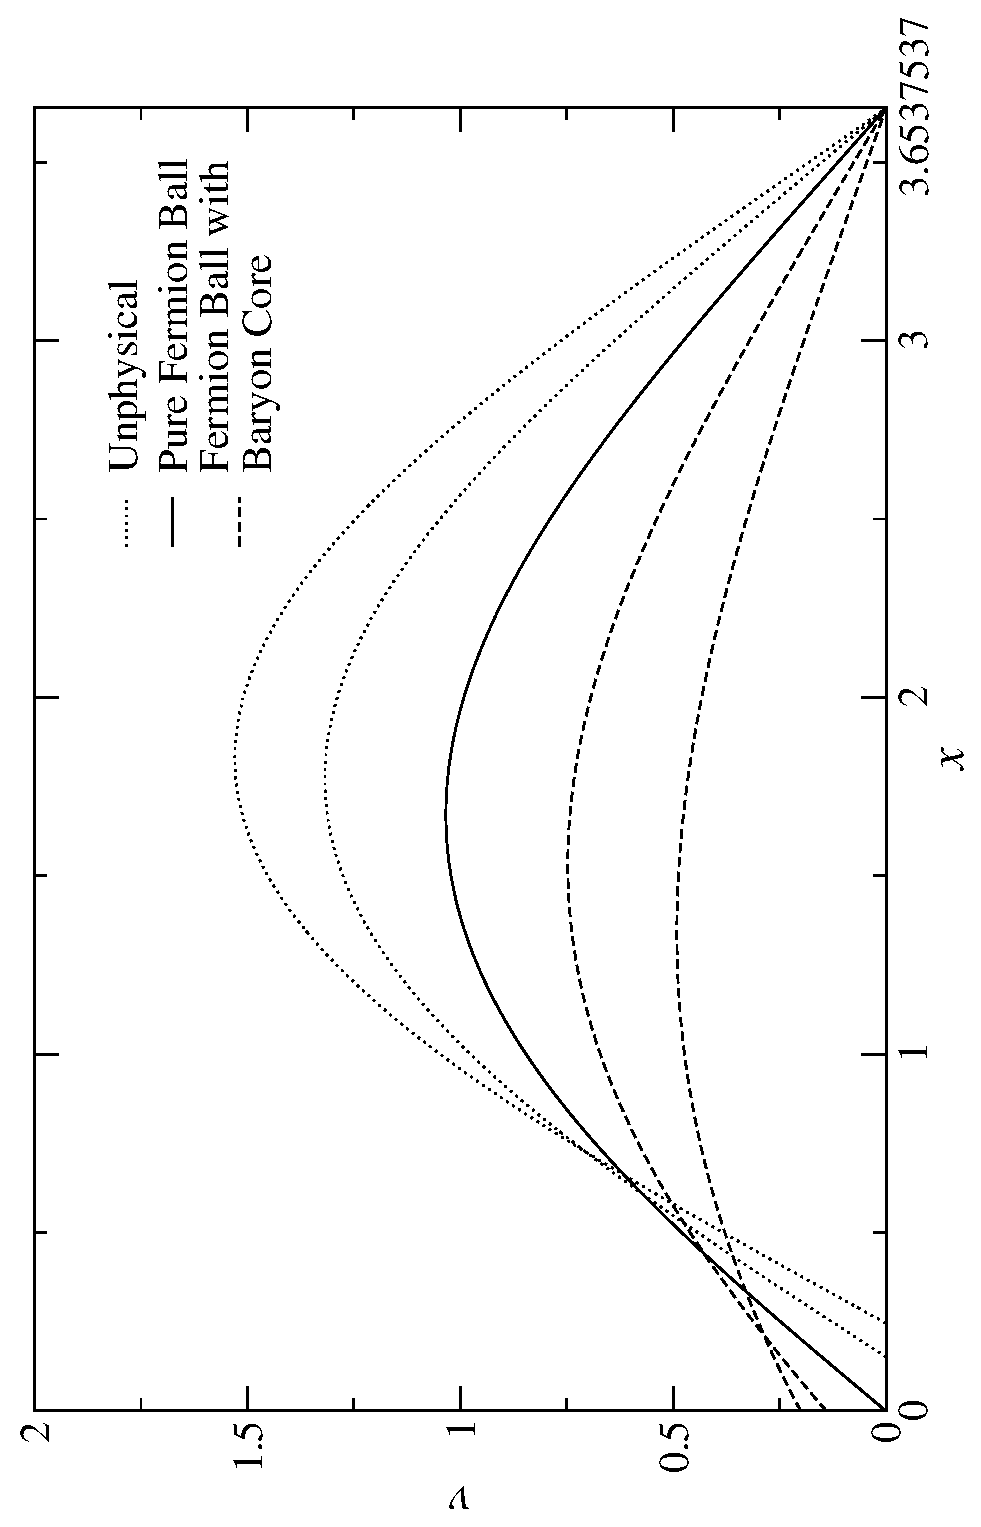
\includegraphics[angle=-90,width=0.9\textwidth]{eps/laneemden.eps}
	\caption{Solutions of the Lan\'e-Emden equation}
	\label{fig_laneemden}
	\end{center}
\end{figure}
The enclosed mass is found at any radius by integrating over the density
\begin{equation}
	M(r) = \int^r_0 4 \pi \rho_\nu (r) r^2 dr
	\label{eqn_classicalmassintegral}
\end{equation}
resulting for any dimensionless radius $x$ as
\begin{equation}
	M(x) = M_\odot\left[v(x)-xv'(x)\right]
	\label{eqn_classicalmass}
\end{equation}
and from (\ref{eqn_classicalarb3}), the gravitational potential is given as
\begin{equation}
	\Phi(x) = \frac{G M_\odot}{a_\nu}\left[v'(x_0)-\frac{v(x)}{x}\right]
	\label{eqn_classicalpotential}
\end{equation}
By the homology theorem, if $v(x)$ is a solution of the Lan\'e-Emden equation, then
\begin{equation}
	\widetilde v(\widetilde x) = A^3 v(Ax)
	\label{eqn_classicalhomology}
\end{equation}
is also a solution, as long as $A$ is a positive real number. This has several implications on the other quantities, and they must
be scaled accordingly. Radii, enclosed mass and gravitational potential scale as
\begin{eqnarray*}
	\widetilde R_0 = \frac{R_0}{A} \qquad
	\widetilde M(\widetilde x) = A^3 M(x) \qquad
	\widetilde \Phi = A^4 \Phi(x)
\end{eqnarray*}
It is then sensible to solve the Lan\'e-Emden equation only once and scale this to the required mass of the fermion ball.
In the numerical solution, an initial value is required for $v'$, whether we choose to solve outward from the origin, or
inward from the outer radius. This is initially set (arbitrarily) to unity, and by solving outward the endpoint value
$x_0$ is obtained, allowing the equation to be solved inward with any $v'(x_0)$, corresponding to a central baryonic
mass given by (before scaling) 
\begin{equation}
	\frac{dv(x_0)}{dx} = - \frac{M_B+M_{\nu \overline{\nu}}}{x_0M_\odot}
	\label{eqn_classicalinitialdvdr}
\end{equation}
Several solutions are shown in Figure \ref{fig_laneemden}.
Using these solutions for $v(x)$ and $v'(x)$, it is now possible with the aid of (\ref{eqn_classicalmass}) and
(\ref{eqn_classicalpotential}) to calculate the mass distribution and potential within the fermion ball. Enclosed mass solutions are
shown in Figure \ref{fig_classicalmassdist}, potentials in Figure \ref{fig_classicalpotential}.

Although in these calculations we have allowed for a baryonic object at the centre, there is no direct evidence to suggest that this
may be the case. A baryonic object must have a
very large mass in order to make a significant impact on the overall mass distribution, for this reason, all further calculations will
assume that $M_B$ is zero, and we therefore have a pure fermion ball.
\begin{figure}[p]
	\begin{center}
	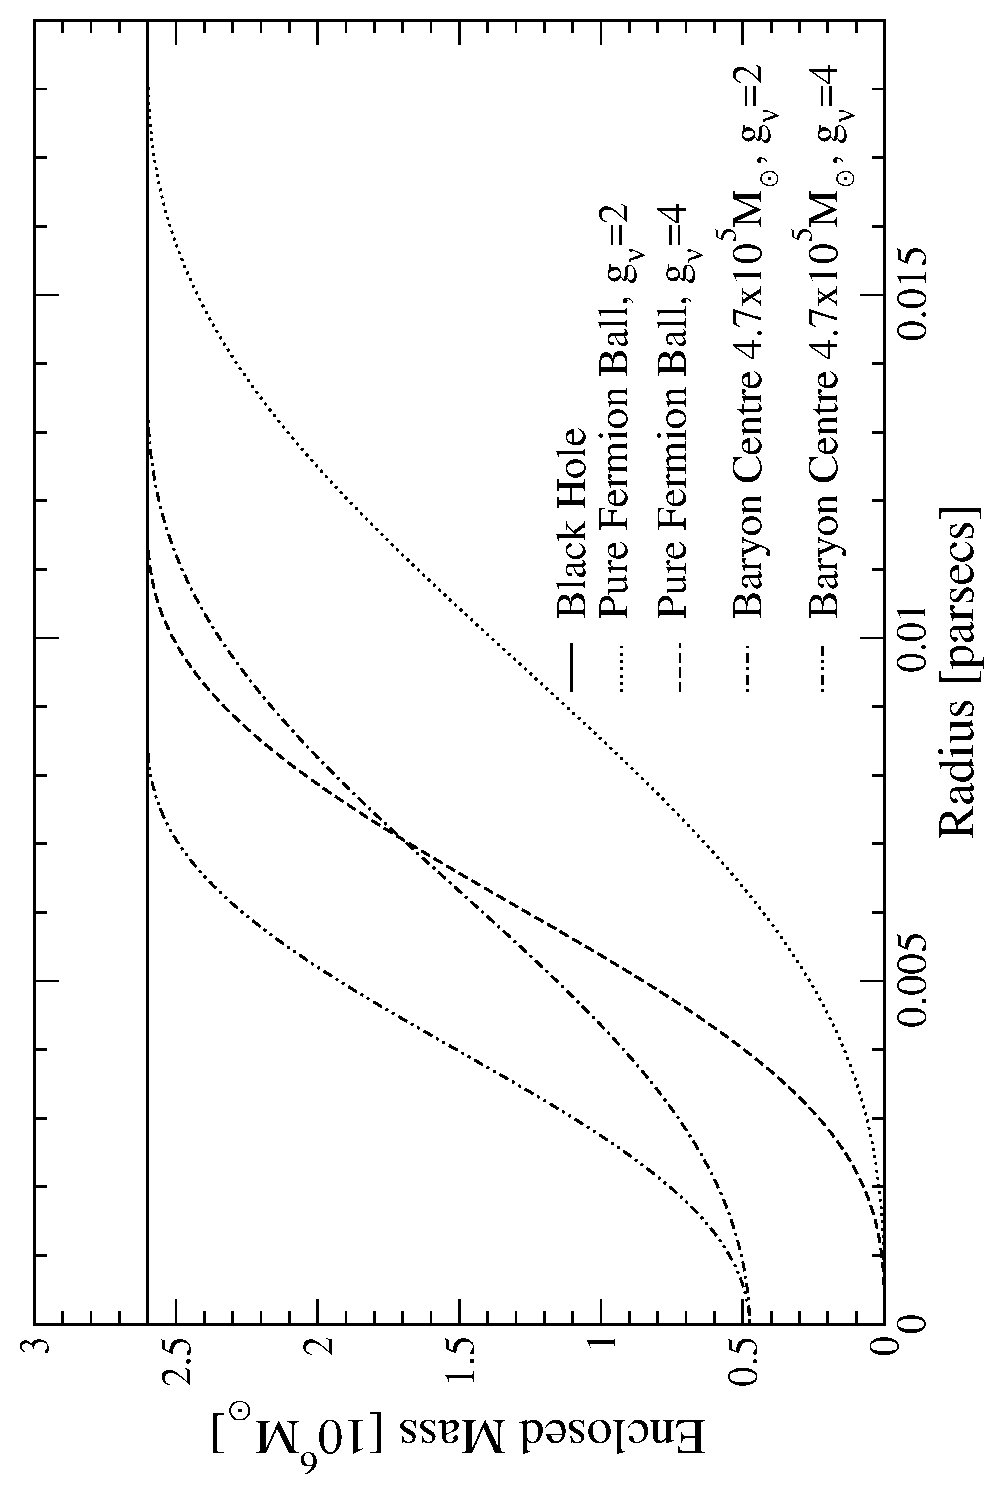
\includegraphics[angle=-90,width=0.9\textwidth]{eps/classicalmassdist.eps}
	\caption{Enclosed mass distribution as a function of radius for 16keV fermions. The solid line denotes a black hole,
	which exhibits a constant enclosed mass at all radii.}
	\label{fig_classicalmassdist}
	\end{center}
\end{figure}
\begin{figure}[p]
	\begin{center}
	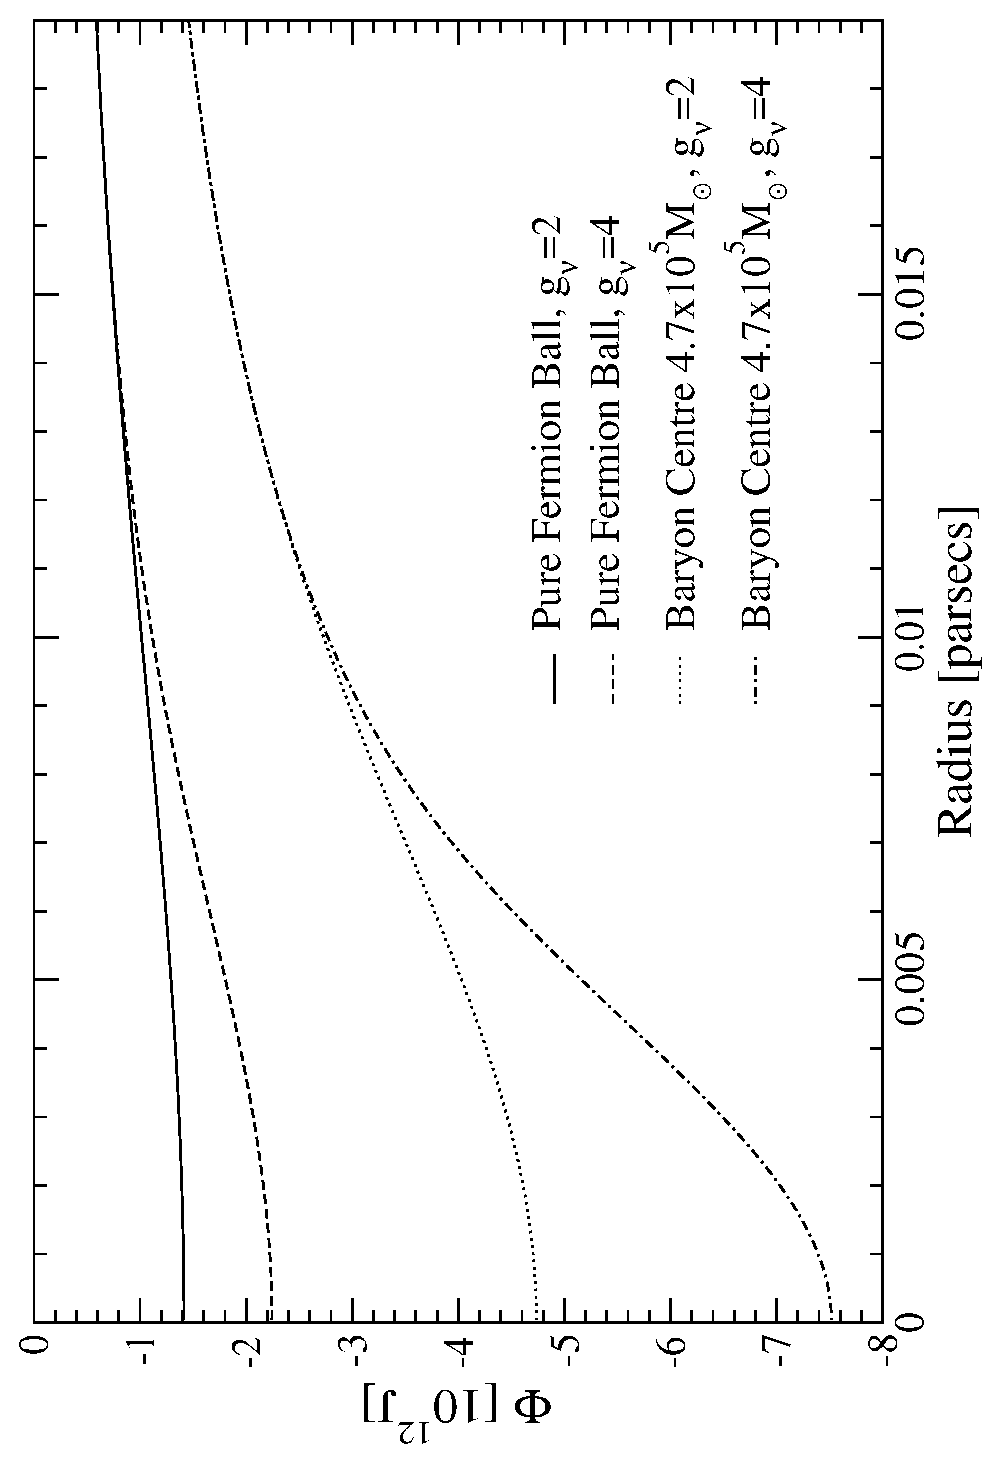
\includegraphics[angle=-90,width=0.9\textwidth]{eps/classicalpotential.eps}
	\caption{Gravitational potential as a function of radius for 16keV fermions.}
	\label{fig_classicalpotential}
	\end{center}
\end{figure}
\subsubsection{Thomas-Fermi}
The Newtonian mass distribution can also be described using the statistical method due to Thomas and Fermi
\cite{ref_thomasfermi}, in which the local Fermi energy is set to the local gravitational binding energy \cite{ref_thomasfermiapproach}.
The Lan\'e-Emden equation (\ref{eqn_laneemden}) has much in common with the Thomas-Fermi equation, containing only an extra negation. The
fermions are gravitationally attractive, opposed to electro-statically repulsive as in atomic physics where the Thomas-Fermi equation is
applied. It is interesting to note that in 1928 Majorana found a semi-analytical solution to the Thomas-Fermi equation which remained
unpublished until 2001 \cite{ref_majoranasolution}, unfortunately the method cannot be directly applied to the Lan\'e-Emden equation.

\subsection{Limits on Fermion Mass}
\label{sec_fermionlimits}
Although these solutions are for 16keV fermions, solutions are easily obtainable for a variety of fermion masses. However, the overall
fermion ball radius and mass is dependent upon the individual rest mass of the fermions and their degeneracy. As such, the minimal
$m_\nu$ in order to constrain the ball fully within the boundaries of a total mass ($M_T$) and a maximal radius ($R_0$) is given by
\begin{equation}
	m_\nu \ge \left( \frac{ - 3 x_0^4 v'(x_0) \pi^2 \hbar^6}{64} \right)^\frac{1}{8} \left(\frac{1}{M_T R_0^3 g_\nu^2}\right)^\frac{1}{8}
	\label{eqn_classicalfermionmass}
\end{equation}

Proper motion analysis \cite{ref_ghezmotion} has imposed an enclosed mass of $2.6 \pm 0.2 \times 10^6 M_\odot$ at a radius of 0.015pc.
Figure \ref{fig_classicalfermionmass} displays several possible mass distributions corresponding to fermion rest masses. It is clear
that when experimental errors are accounted for, the minimal allowed $m_\nu$ is approximately 16keV. For this reason, all calculations
from here on in will be performed using 16keV fermions. This is based on the assumption that the fermion ball is fully constrained
within the 0.015pc, a more massive fermion ball with fermions of lesser $m_\nu$ would still reproduce the results of
\cite{ref_ghezmotion}, and this may be important later.
\begin{figure}[!tb]
	\begin{center}
	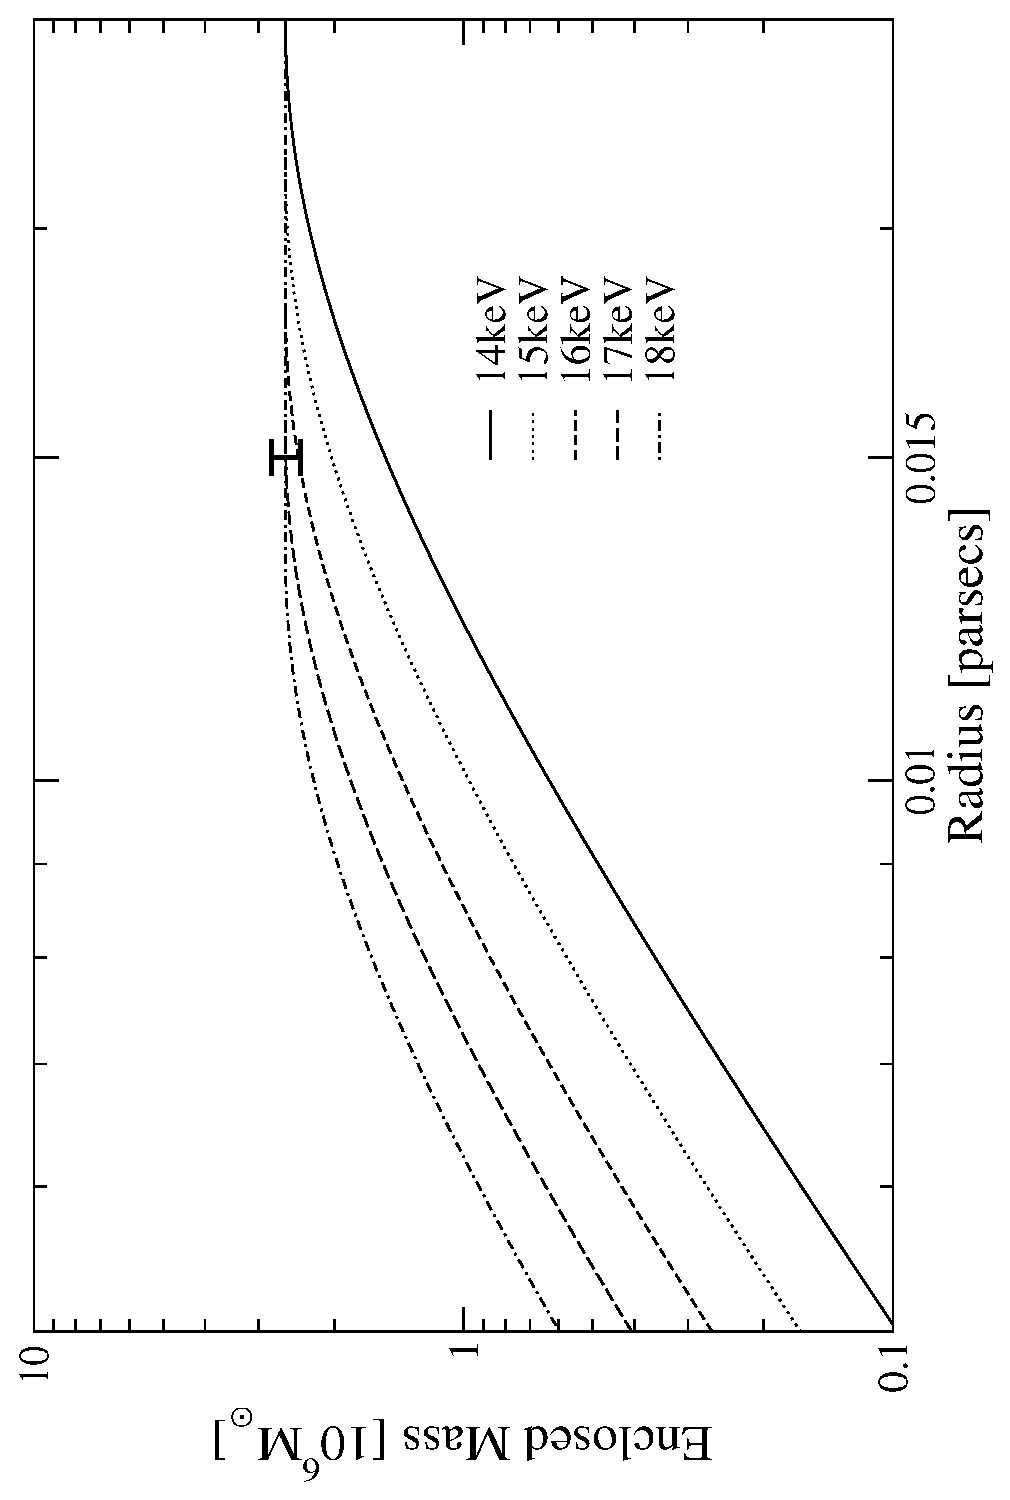
\includegraphics[angle=-90,width=0.9\textwidth]{eps/classicalfermionmass.eps}
	\caption{The enclosed mass as a function of radius for various fermion masses. Data point is from \cite{ref_ghezmotion}.}
	\label{fig_classicalfermionmass}
	\end{center}
\end{figure}
It is also worth noting that the mass distribution for $g_\nu=2$ fermions can easily be reproduced for $g_\nu=4$ by slightly
decreasing the rest mass according to
\begin{equation}
	m_\nu g_\nu^{\frac{1}{4}} = \overline{m}_\nu \overline{g}_\nu^{\frac{1}{4}}
	\label{eqn_classicalfermiondegeneracyrelation}
\end{equation}

\section{Relativistic Mass Distribution}
\begin{quotation}
	\raggedleft \it The probability of them visiting is directly proportional\\ to how much you feel like being left alone \\
-- Einstein's Theory of Relatives
\end{quotation}
In the previous section, a Newtonian description for the fermion ball mass distribution was outlined. When large
masses are involved in calculations, it is often advisable to confirm the results with a relativistic treatment \cite{ref_bilic}, and
that is what this section will serve to provide. We choose to use units such that the speed of light and gravitational constant
are unity ($c=G=1$) and begin by assuming spherical symmetry of the fermion ball and a static solution, allowing the use of the
Schwarzschild metric
\begin{equation}
	ds^2=e^{\nu(r)}dt^2 - e^{\lambda(r)}dr^2 - r^2d\theta^2 - r^2 \sin^2\theta d\phi^2
	\label{eqn_schwarzschild}
\end{equation}
Using Einstein's field equations we obtain
\begin{equation}
	-8 \pi T_{\mu \nu} = R _{\mu \nu} - \frac{1}{2} R g_{\mu \nu} + \Lambda g_{\mu \nu}
	\label{eqn_einstein}
\end{equation}
The solutions to the field equations \cite{ref_tolmanpaper} are
\begin{eqnarray}
	&& 8 \pi T_0^0 = e^{- \lambda} \left(\frac{\lambda'}{r} - \frac{1}{r^2} \right) + \frac{1}{r^2} - \Lambda
	\label{eqn_einsteinsoln1} \\
	&& 8 \pi T_1^1 = - e^{- \lambda} \left(\frac{1}{r^2} - \frac{\nu'}{r} \right) + \frac{1}{r^2} - \Lambda
	\label{eqn_einsteinsoln2} \\
	&& 8 \pi T_2^2 = 8 \pi T_3^3 = \frac{e^{- \lambda}}{2} \left(\nu'' + \frac{\nu'^2}{2} + \frac{\nu'}{r} - \frac{\lambda'\nu'}{2}
	-\frac{\lambda'}{r} \right)
	\label{eqn_einsteinsoln3}
\end{eqnarray}
The approach to solving the relativistic mass distribution is to first solve the equation of hydrostatic equilibrium, interior and
exterior to the fermion ball and then to introduce the relativistic equation of state for a Fermi gas.

\subsection{Hydrostatic Equilibrium}
The fermion ball is treated as a perfect fluid \cite{ref_tolmanbook}
\begin{equation}
	T^{\mu \nu} = \frac{\partial x^\mu}{\partial x_0^\alpha} \frac{\partial x^\nu}{\partial x^\beta} T_0^{\alpha \beta}
	\label{eqn_relativisticfluid}
\end{equation}
which by definition is incapable of exerting transverse stress. Therefore the quantities of proper mass density $\rho_0(r)$
and proper hydrostatic pressure $P_0(r)$ may be defined as
\begin{eqnarray}
	&& T_0^{00} = \rho_0(r)
	\label{eqn_relativisticpropermassdensity} \\
	&& T_0^{11} = T_0^{22} = T_0^{33} = P_0(r)
	\label{eqn_relativisticproperpressure}
\end{eqnarray}
The only observable component of stress for a local observer will be the proper hydrostatic pressure. It follows that the
energy-momentum tensor becomes
\begin{equation}
	T^{\mu \nu} = \frac{\partial x^\mu}{\partial x_0^0}\frac{\partial x^\nu}{\partial x_0^0} \rho_0
		    + \frac{\partial x^\mu}{\partial x_0^1}\frac{\partial x^\nu}{\partial x_0^1} P_0
		    + \frac{\partial x^\mu}{\partial x_0^2}\frac{\partial x^\nu}{\partial x_0^2} P_0
		    + \frac{\partial x^\mu}{\partial x_0^3}\frac{\partial x^\nu}{\partial x_0^3} P_0
	\label{eqn_relativisticlocalpressure}
\end{equation}
where $x_0^0, x_0^1...$ are 'proper' coordinates and $x^0, x^1...$ are the points of interest. Also
\begin{equation}
	g^{\mu \nu} = \frac{\partial x^\mu}{\partial x_0^\alpha}\frac{\partial x^\nu}{\partial x_0^\beta} g_0^{\alpha \beta}
	\label{eqn_relativisticgnumu}
\end{equation}
reduces to
\begin{equation}
	\frac{d x^\mu}{ds} = \frac{\partial x^\mu}{\partial x_0^0}
	\label{eqn_relativisticgnumureduced}
\end{equation}
Inserting (\ref{eqn_relativisticgnumureduced}) into (\ref{eqn_relativisticlocalpressure}) gives
\begin{eqnarray}
	&T^{\mu \nu} =& (\rho_0 + P_0) \frac{dx^\mu}{ds} \frac{dx^\nu}{ds} - g^{\mu \nu} P_0 \nonumber \\
	\therefore \qquad &T_\mu^{\nu \phantom{\mu}} =& (\rho_0 + P_0) g_{\alpha \mu} \frac{dx^\alpha}{ds} \frac{dx^\nu}{ds} - g_\mu^\nu P_0
	\label{eqn_relativisticenergysoln}
\end{eqnarray}
In our static case we have
\begin{eqnarray}
	\frac{dt}{ds} &=& e^{-\frac{\nu}{2}}
	\label{eqn_relativisticstatic1} \\
	\frac{dr}{ds} &=& \frac{d\theta}{ds} = \frac{d\phi}{ds} = 0
	\label{eqn_relativisticstatic2}
\end{eqnarray}
which leads to
\begin{eqnarray}
	&& T_0^0 =  \rho_0
	\label{eqn_relativisticstatic3} \\
	&& T_1^1 =  T_2^2 = T_3^3 = -P_0
	\label{eqn_relativisticstatic4}
\end{eqnarray}
From (\ref{eqn_relativisticstatic4}), (\ref{eqn_einsteinsoln3}) and (\ref{eqn_einsteinsoln1}) we arrive at the relativistic
solution for hydrostatic equilibrium
\begin{equation}
	\frac{dP_0}{dr} + (\rho_0 + P_0) \frac{\nu'}{2} = 0
	\label{eqn_relativisticpressuredensitysolution}
\end{equation}
which is comparable to the Newtonian solution (\ref{eqn_hydroequil}).

\subsubsection{Exterior Solution (Schwarzschild)}
In empty space, all components of $T_\mu^\nu$ are zero. So by relating $T_0^0=T_1^1$ (\ref{eqn_einsteinsoln1}) and
(\ref{eqn_einsteinsoln2}), it is clear that $\lambda'=-\nu'$. Again, relating to $T_2^2$ (\ref{eqn_einsteinsoln3}) it follows
that
\begin{equation}
	\nu'' + \nu'^2 + \frac{2\nu'}{r} =0
	\label{eqn_relativisticarb1}
\end{equation}
which has a solution in the form
\begin{equation}
	e^\nu = a + \frac{b}{r}
	\label{eqn_relativisticarb2}
\end{equation}
Using the special relativity metric and restoring the correct units
\begin{equation}
	e^{-\lambda} = 1 - \frac{2 G M}{c^2 r}
	\label{eqn_relativisticarb3}
\end{equation}
where $M$ is the total mass.

\subsubsection{Interior Solution (Oppenheimer and Volkoff)}
This solution was originally formulated in \cite{ref_oppenheimervolkoff} as a means to explore the physics of massive neutron
cores. Due to the presence of the fermions, we can no longer make the equality between (\ref{eqn_einsteinsoln1}),
(\ref{eqn_einsteinsoln2}) and (\ref{eqn_einsteinsoln3}) as in the exterior solution, $T_\mu^\nu$ is now non-zero. By using a
trial and error approach and introducing a variable which has the form
\begin{equation}
	u(r) = \frac{r}{2}\left(1-e^{-\lambda}\right)
	\label{eqn_relativisticarb4}
\end{equation}
the $T_0^0$ solution (\ref{eqn_einsteinsoln1}) then becomes
\begin{equation}
	\frac{du}{dr} = 4 \pi \rho_0 r^2
	\label{eqn_relativisticarb5}
\end{equation}
At the outer radius ($R$, which must be continuous with the exterior solution), we see that
\begin{equation}
	u_R = \frac{R}{2}\left(1-e^{-\lambda(R)}\right) = M
	\label{eqn_relativisticarb6}
\end{equation}
So the solution to $e^{-\lambda}$ is the same for both the interior and the exterior (\ref{eqn_relativisticarb3}). Re-inserting the
correct units, $T_1^1$ (\ref{eqn_einsteinsoln2}) becomes
\begin{equation}
	\frac{dP_\nu}{dr} = - \frac{G}{r^2} \left(\frac{ \rho_0+ \frac{P_\nu}{c^2}}{r-2u}\right) \left( m + \frac{4 \pi P_\nu r^3}{c^2} \right)
	\label{eqn_relativisticarb7}
\end{equation}

\subsection{Equation of State for a Relativistic Degenerate Fermi Gas}
This is by far the simplest approach to derive the equation of state for a relativistic degenerate Fermi gas \cite{ref_chandra}.
We begin by confining $N$ fermions in a volume $V$. The number of quantum states with momentum between $p$ and $p+dp$ is given by
\begin{equation}
	\frac{4 V \pi g_\nu p^2 dp}{h^3}
	\label{eqn_chandra1}
\end{equation}
Pauli's exclusion principle implies
\begin{equation}
	N(p)dp \le \frac{4 V \pi g_\nu p^2 dp}{h^3}
	\label{eqn_chandra2}
\end{equation}
A completely degenerate gas has all lowest states occupied
\begin{equation}
	N(p) = \frac{4 V \pi g_\nu p^2}{h^3}
	\label{eqn_chandra3}
\end{equation}
If there is a finite number $N$ of fermions, then they must all have momentum less than the Fermi momentum $p_0$ such that
\begin{equation}
	N = \frac{4 V \pi g_\nu}{h^3} \int_0^{p_0}p^2dp = \frac{4 V \pi g_\nu p_0^3}{3 h^3}
	\label{eqn_chandra4}
\end{equation}
The Fermi momentum is related to number density by
\begin{equation}
	n = \frac{N}{V} = \frac{4 \pi g_\nu p_0^3}{3 h^3}
	\label{eqn_chandra5}
\end{equation}
The pressure is the mean rate of transfer of momentum across an ideal surface of unit area, from this we obtain
\begin{equation}
	PV=\frac{1}{3} \int_0^{\infty}N(p)pv_pdp
	\label{eqn_chandra6}
\end{equation}
where $v_p$ is the associated velocity, this leads to
\begin{equation}
	P=\frac{4\pi g_\nu}{3h^3} \int_0^{p_0}p^3\frac{\partial E}{\partial p}dp
	\label{eqn_chandra7}
\end{equation}
The internal energy of the gas (due to translational energy of the motions of individual fermions) is
\begin{equation}
	U=\int_0^\infty N(p) E dp
	\label{eqn_chandra8}
\end{equation}
for complete degeneracy we get
\begin{eqnarray}
	&&U=\frac{4V\pi g_\nu}{h^3} \int_0^{p_0} E p^2 dp
	\label{eqn_chandra9} \\
	\therefore &&P = \frac{4\pi g_\nu}{3h^3} E(p_0)p_0^3 - \frac{U}{V}
	\label{eqn_chandra10}
\end{eqnarray}
and according to special relativity
\begin{eqnarray}
	&&E = mc^2\left(\sqrt{1+\frac{p^2}{m_\nu^2 c^2}}-1\right)
	\label{eqn_chandra11} \\
	&&\frac{\partial E}{\partial p} = \frac{1}{m_\nu} \left( 1 + \frac{p^2}{m_\nu^2c^2}\right)^{-\frac{1}{2}} p
	\label{eqn_chandra12}
\end{eqnarray}
Inserting into (\ref{eqn_chandra7}) we arrive at
\begin{equation}
	P = \frac{4\pi g_\nu}{3 m_\nu h^3} \int_0^{p_0} \frac{p^4 dp}{\sqrt{1+\frac{p^2}{m_\nu^2 c^2}}}
	\label{eqn_chandra13}
\end{equation}
By substituting $\sinh \theta = \frac{p}{mc}$ we get
\begin{eqnarray}
	P &=& \frac{4\pi g_\nu m_\nu^4c^5}{3h^3} \int_0^{\theta_0} \sinh^4 \theta d\theta \nonumber \\
	  &=& \frac{4\pi g_\nu m_\nu^4c^5}{3h^3} \left[ \frac{\sinh^3\theta \cosh \theta}{4} -\frac{3 \sinh 2\theta}{16} + \frac{3\theta}{8} \right]_{\theta = \theta_0}
	\label{eqn_chandra14}
\end{eqnarray}
By making the following substitution, in order that we may use a more convenient unit in dealing with Fermi momentum
\begin{equation}
	X=\frac{p_0}{m_\nu c}
	\label{eqn_relatfermibetterunits}
\end{equation}
and using $\sinh^{-1}X=\ln(X+\sqrt{1+X^2})$, (\ref{eqn_chandra14}) reduces to
\begin{equation}
	P = K \left[ X\left(1+X^2\right)^{\frac{1}{2}}\left(\frac{2}{3}X^2-1\right) + \ln \left(X+\left(1+X^2\right)^{\frac{1}{2}}\right)\right]
	\label{eqn_chandra15}
\end{equation}
where
\begin{equation}
	K = \frac{g_\nu m_\nu^4 c^5}{16\pi^2\hbar^3}
	\label{eqn_chandra16}
\end{equation}
Noting that the mass energy density is given by the internal energy density plus the addition of all the fermion rest mass energies, we get
\begin{equation}
	\rho = \frac{U}{Vc^2} + nm
	\label{eqn_chandra17}
\end{equation}
Working from (\ref{eqn_chandra17}), (\ref{eqn_chandra10}) and (\ref{eqn_chandra5}) we obtain the relativistic equation of state for
a Fermi gas, concerning the proper mass density
\begin{equation}
	\rho = \frac{K}{c^2}\left[X\left(2X^2+1\right)\left(1+X^2\right)^{\frac{1}{2}} - \ln \left( X+\left( 1+X^2\right)^{\frac{1}{2}}\right) \right]
	\label{eqn_chandra18}
\end{equation}
Equations (\ref{eqn_chandra15}), (\ref{eqn_chandra16}) and (\ref{eqn_chandra18}) fulfil our requirements for the degenerate relativistic
equation of state for a Fermi gas.

\subsection{Mass Distribution}
\label{sec_relatmassdist}
Now that we have formulated the equation of hydrostatic equilibrium and the equation of state for a degenerate relativistic Fermi gas,
we may combine them in order to find the mass distribution of the fermion ball. By using the dimensionless units
\begin{equation}
	x=\frac{r}{b_\nu} \qquad \mu = \frac{m}{d_\nu}
	\label{eqn_relatmassdistunits}
\end{equation}
where
\begin{equation}
	b_\nu = \sqrt{\frac{4 \pi \hbar^3}{G g_\nu m_\nu^4 c}} \qquad d_\nu = 2\sqrt{\frac{4 \pi \hbar^3 c^3}{G^3 g_\nu m_\nu^4}}
	\label{eqn_relatdimensionless}
\end{equation}
It is possible to obtain the mass distribution from (\ref{eqn_relativisticarb7}), (\ref{eqn_chandra16}) and (\ref{eqn_chandra18}) by
integrating over the density as in the Newtonian solution (\ref{eqn_classicalmassintegral}).
\begin{align}
	\frac{dX}{dx} = - &\frac{1+X^2}{X\left(x^2 - 2\mu x\right)} \nonumber \\
			  &\left\{ \mu +x^3 \left[ X\left(1+X^2\right)^{\frac{1}{2}}
			  \left(\frac{2}{3}X^2-1\right) + \ln \left(X + \left( 1+X^2\right)^{\frac{1}{2}} \right)\right]\right\}
	\label{eqn_relativisticxsolution} \\
	\frac{d\mu}{dx} = x^2&\left\{ X\left( 1+X^2\right)^{\frac{1}{2}} \left(2X^2+1\right)
			  - \ln \left(X + \left( 1+X^2\right)^{\frac{1}{2}} \right)\right\}
	\label{eqn_relativisticmusolution}
\end{align}
And again, as in the Newtonian case, these equations must be solved numerically. As we have no
need for inserting a baryon core, we simply set $\mu(x_0)=0$ and select a value for the Fermi momentum $X(x_0)$. This allows for calculation
of the total mass and radius of the fermion ball from a single parameter (besides the fermion characteristics), but has the
disadvantage of requiring a trial and error technique when selecting total mass. Solutions for $X$, $\mu$ and $\mu'$ are presented in
Figure \ref{fig_relativisticsolution}.
\begin{figure}[!p]
	\begin{center}
	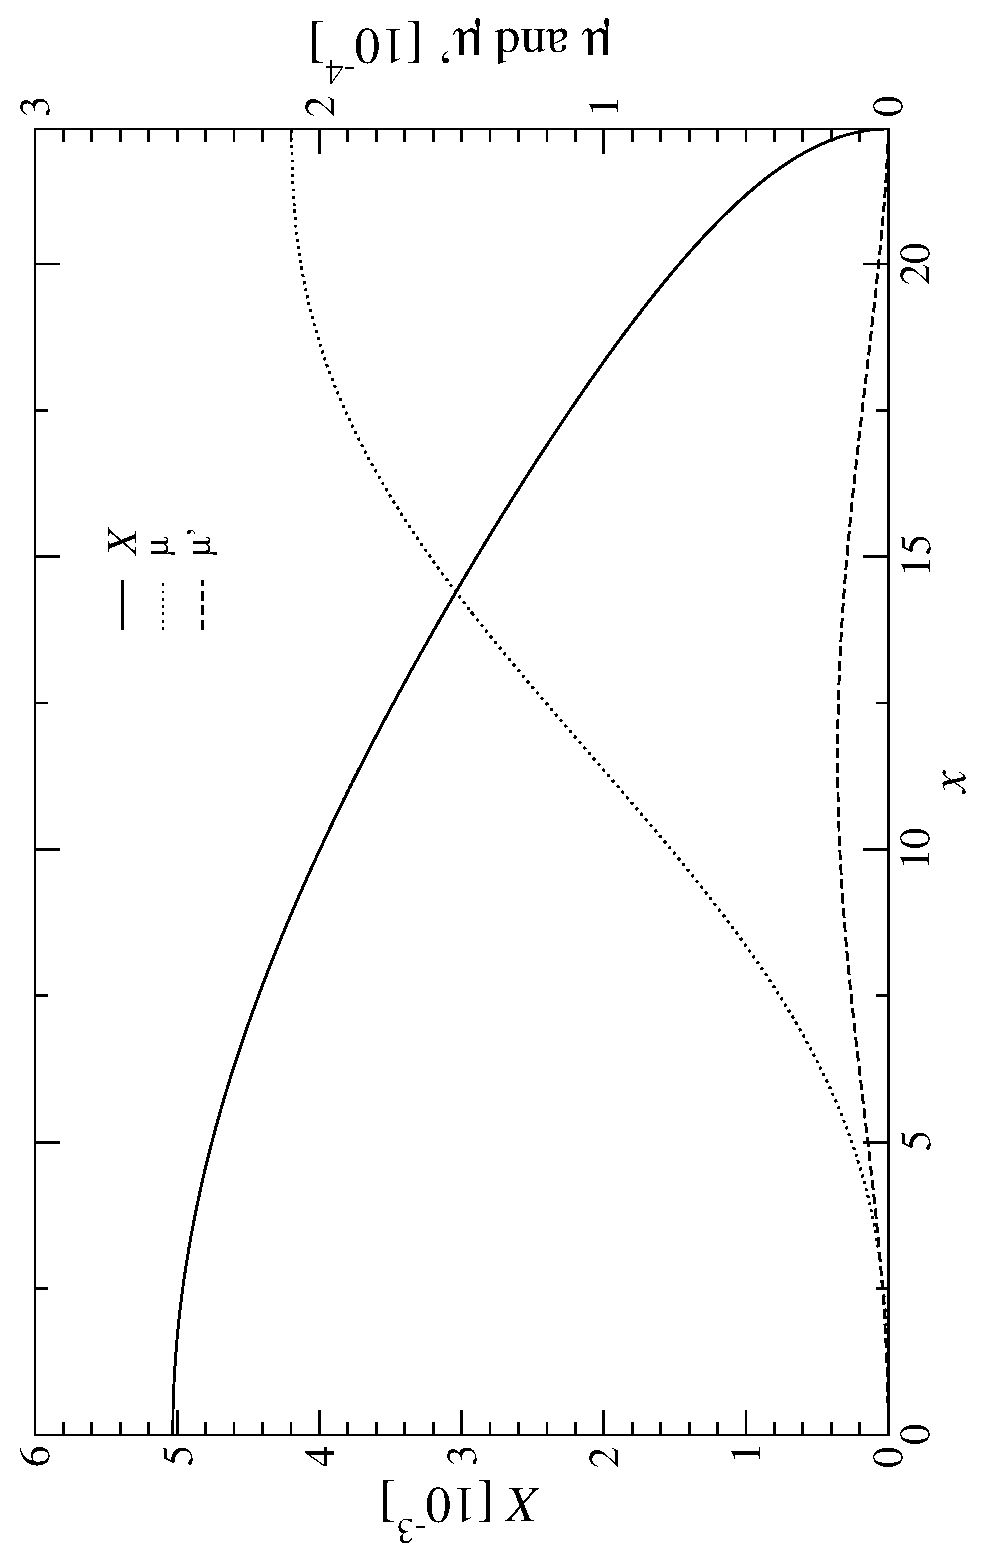
\includegraphics[angle=-90,width=0.9\textwidth]{eps/relativisticsolution.eps}
	\caption{Relativistic solution of the dimensionless mass $\mu$, derivative $\mu'$ and Fermi momentum $X$ as functions of the
	dimensionless radius.}
	\label{fig_relativisticsolution}
	\end{center}
\end{figure}

It is enlightening to find that the relativistic derivation of the mass distribution has confirmed the classical method.
For this reason, graphs of mass
distribution will not be shown as they are identical to those in Section \ref{sec_classical}. However, the relativistic approach has been
useful, as it has also revealed more information about the fermion ball. It is now possible to plot a relativistic relation
between total mass and radius (Figure \ref{fig_relativisticmvsr}) and has also given an alternative numerical technique for calculating
$M$ and $M'$, in fact this method turns out to be preferred in the spectra simulations of Section \ref{sec_accretion}.

It is clear from the mass-radius plot that the fermion ball is indeed non-relativistic, as relativistic
effects are only prevalent near the Oppenheimer-Volkoff limit, which is a factor of $10^3$ larger than the mass of the centre of our galaxy.
The Oppenheimer-Volkoff limit is the maximal mass which a degenerate fermion ball can have.
It is noteworthy that this Oppenheimer-Volkoff limit is very much comparable to the mass of the largest
observed super-massive, compact, dark object which is $3\times 10^9M_\odot$; M87 in the Virgo cluster \cite{ref_centralobjects}.
\begin{figure}[!p]
	\begin{center}
	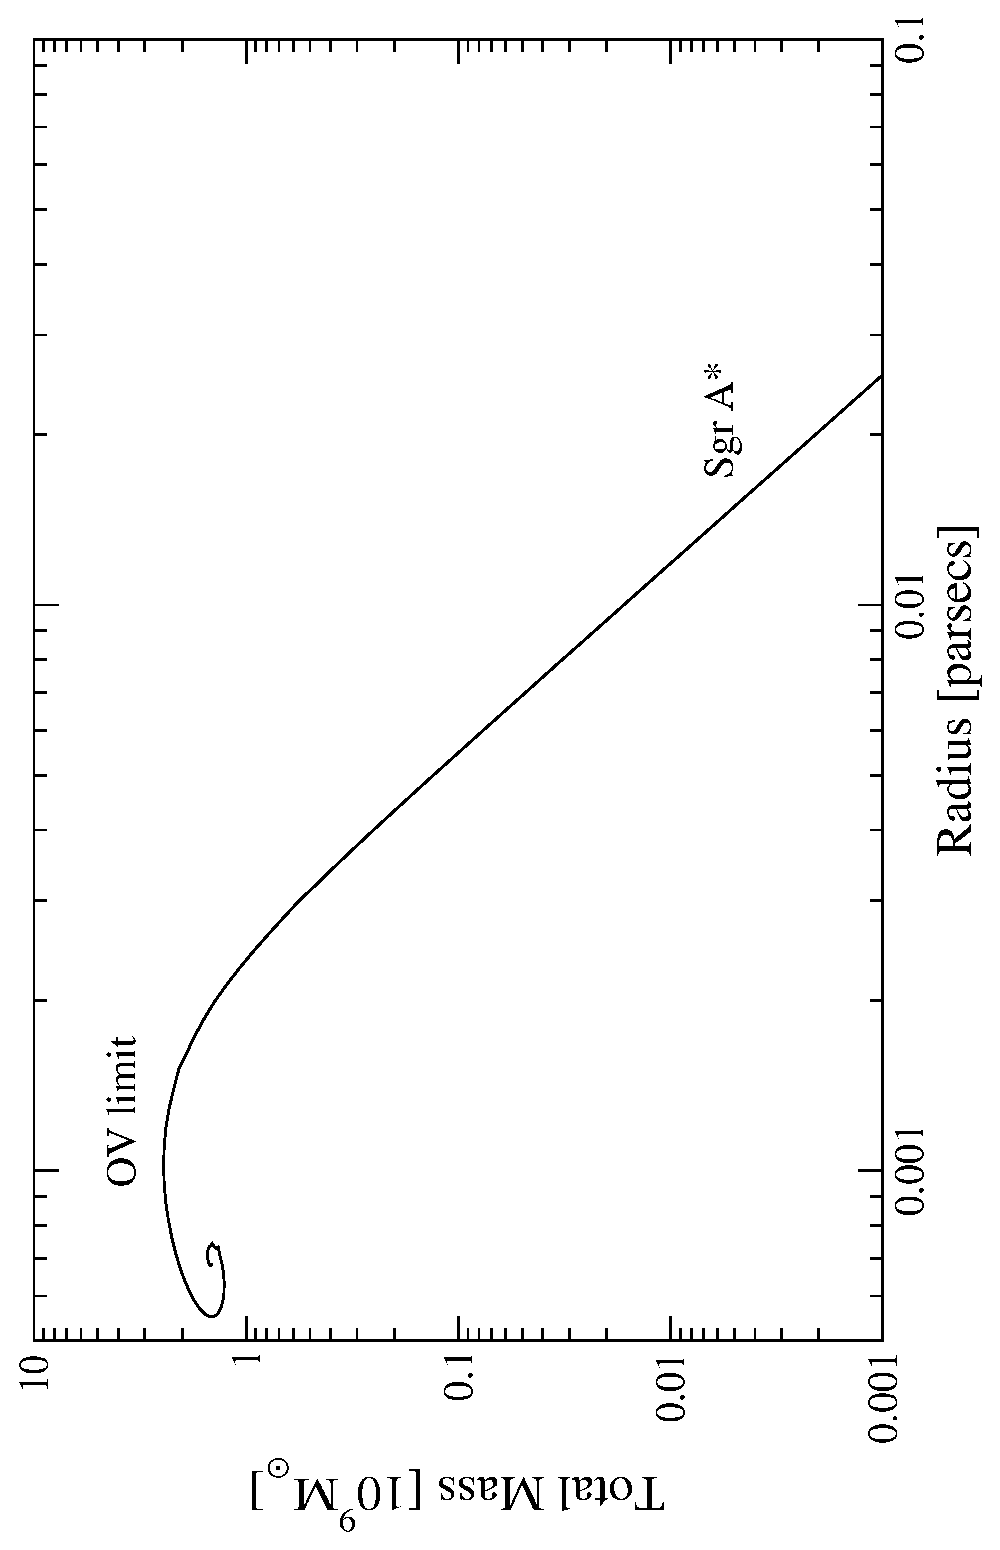
\includegraphics[angle=-90,width=0.9\textwidth]{eps/relativisticmvssr.eps}
	\caption{Relativistic mass-radius relation. Note the turning point is the Oppenheimer-Volkoff limit (2.45$\times 10^9 M_\odot$)
	and the curve left of the maximum represents unstable configurations curling around the point of infinite central density.
	The mass-radius region which the centre of our galaxy lies within is noted as Sgr A*. As previously decided upon, this
	is for 16keV, $g_\nu=2$ fermions.}
	\label{fig_relativisticmvsr}
	\end{center}
\end{figure}

\section{Formation of a Fermion Ball}
\begin{quotation}
	\raggedleft \it
	We are all agreed that your theory is crazy.\\
	The question which divides us is whether it is\\
	crazy enough to have a chance of being correct.\\
	-- Niels Bohr
\end{quotation}
Thus far, we have argued that a fermion ball is possible, provided a 16keV fermion exists in nature. Candidates for such a fermion
and their origins have also been briefly mentioned. Another requirement of the theory is that such a fermion ball may be formed. This
section aims to show that it is possible to create such an object by closely following the work of \cite{ref_formation}.

\subsection{Analogy to a Boson Star}
To understand the formation of a fermion ball, we first study the analysis of self-interacting scalar fields, often called boson stars
\cite{ref_bosonform}.
We then use scaling arguments to make an equivalence to a certain type of cold boson star.

Consider a complex scalar field $\Psi$ with a repulsive Lagrangian interaction term $U(|\Psi|^2)$. By introducing the dimensionless
parameter $\Lambda$, we define the length and mass scales as
\begin{equation}
	R_*=\frac{\Lambda}{m}=\frac{\lambda m_{pl}}{m^2} \qquad \qquad M_*=R_*m^2_{pl}
	\label{eqn_formscales}
\end{equation}
where $m_{pl}=\sqrt{G}^{-1}$ is the Planck mass. In the Newtonian limit, a self-gravitating boson star is governed by the
dimensionless Gross-Pitaevskii like equations
\begin{eqnarray}
	\Delta \phi &=& |\Psi|^2 \label{eqn_formpoisson} \\
	\frac{i}{\Lambda} \frac{\partial \Psi}{\partial t} &=& \left[ -\frac{\Delta}{2\Lambda^2} + \phi + V(|\Psi|^2) \right]
		\Psi \label{eqn_formbig} \\
	\rho &=& \frac{m^4}{4\pi \lambda^2} |\Psi|^2 \label{eqn_formrho}
\end{eqnarray}
where we have introduced the dimensionless potential
\begin{equation}
	V(|\Psi|^2) = \frac{4\pi \lambda^2}{m^4}\frac{dU}{d|\Psi|^2}
	\label{eqn_formv}
\end{equation}
The pressure tensor in these dimensionless units is given by
\begin{equation}
	P_{ij}= \frac{m^4}{4\pi\lambda^2 \Lambda^2}
		\left( \rm{Re}\frac{\partial\Psi}{\partial x_i} \frac{\partial\Psi^*}{\partial x_j}
			-\delta_{ij}\frac{\Delta|\Psi|^2}{4} \right)
		+\delta_{ij}\left(|\Psi|^2\frac{d U}{d |\Psi|^2} -U \right)
	\label{eqn_formpressuretensor}
\end{equation}
A static, spherically symmetric solution is obtained with the ansatz
\begin{equation}
	\Psi = e^{- i \epsilon R_* t} \Phi(r)
	\label{eqn_formpsiphi}
\end{equation}
where $\Phi(r)$ is a real function. It is clear that for large $\Lambda$, (\ref{eqn_formbig}) and (\ref{eqn_formpsiphi}) reduce to
\begin{equation}
	\frac{\epsilon}{m} - \phi - V = 0
	\label{eqn_formereduce}
\end{equation}
This solution is exact in the limit $\Lambda \rightarrow \infty$, which is the Thomas-Fermi limit \cite{ref_bosonformtf}. In this limit,
(\ref{eqn_formpressuretensor}) becomes diagonal with $P = P_{ii}$. We obtain an equation of state given by (\ref{eqn_formrho}) and
\begin{equation}
	P=\rho V(\rho) - U(\rho)
	\label{eqn_formpressure}
\end{equation}
Equations (\ref{eqn_formereduce}) and (\ref{eqn_formpressure}) yield the equation of hydrostatic equilibrium
\begin{equation}
	\frac{dP}{\rho}=-d\phi
	\label{eqn_formpressurephi}
\end{equation}
If the equation of state is given as the polytropic type
\begin{equation}
	P(\rho)=K\rho^{1+\frac{1}{n}}
	\label{eqn_formpolytropic}
\end{equation}
we can determine the potential $U$ and $V$ by integrating (\ref{eqn_formpressurephi}). It can therefore be shown that
Equation (\ref{eqn_formpressurephi}) is equal to $V$, which yields
\begin{equation}
	V=(n+1)K\rho^{\frac{1}{n}}
	\label{eqn_formvrho}
\end{equation}
If we fix $\lambda$ in a convenient manner, we get the potential
\begin{equation}
	V=|\Psi|^{\frac{n}{2}}
	\label{eqn_formpotential}
\end{equation}
The polytropic equation of state with $n=\frac{3}{2}$, together with (\ref{eqn_formpressurephi}) and (\ref{eqn_formpoisson}) (the dimensionless
Poisson equation), describe a fermion ball. This has demonstrated that a fermion ball is equivalent to a boson star in the limit
$\Lambda \rightarrow \infty$. It has been shown numerically \cite{ref_bosonform} that even for moderate values of $\Lambda$, the static
solutions are almost degenerate and are quite well approximated by the static solution for an infinite $\Lambda$.

\subsection{Time Evolution of the Collapse}
The basic regulating mechanism is the kinetic part of (\ref{eqn_formbig}), which penalises density spikes. The criterion for simulation
is that the ratio of kinetic and pressure contributions to the static energy functional should be small. Great care must be taken during
numeric simulation to ensure that the self-interaction term $V$ is not dominated by the other terms. If this occurs, there is a
crossover to mini boson star behaviour.

An evolution plot for collapsing fermionic matter ball is shown in Figure \ref{fig_robert}.
To prevent matter from being artificially reflected by the radius boundary, an $r$-dependant imaginary `sponge' has been introduced.
This sponge removes the ejected fermionic matter.
\begin{figure}[t]
	\begin{center}
	\includegraphics[angle=-90,width=0.9\textwidth]{eps/robert.eps}
	\caption{Combined contour-density plot for the evolution of $|r \Psi |^{2}$. Green contour lines denote levels from
	$10^{-5}$ to $10^{-4}$ while red lines denote levels below $10^{-5}$.
	Gravitational collapse is followed by an ejection of excess matter leaving a fermion ball at the centre
	\cite{ref_formation}.}
	\label{fig_robert}
	\end{center}
\end{figure}

In summary, using a bosonic representation of the dynamical Thomas-Fermi theory for a self-gravitating gas, it can be shown that
non-relativistic, degenerate fermionic matter will form a super-massive fermion ball through gravitational collapse accompanied by ejection.

\section{Dynamics of Stars near the Galactic Centre}
\begin{quotation}
	\raggedleft \it The computer can't tell you the emotional story. \\ It can give you the exact mathematical design, \\
	but what's missing are the eyebrows. \\ -- Frank Zappa
\end{quotation}
The best way to probe a distribution of mass when it does not emit very strongly, is to observe the orbits of objects moving
through that distribution. Luckily the orbits of stars near the centre of the galaxy have been spatially resolved
\cite{ref_ghezorbits, ref_eckartorbits} and we may therefore use this data to compare with motion predictions from computer
simulations using the fermion ball mass distribution. But as there are a lot of stars neighbouring the central object, we must
first decide which to concentrate our efforts upon. Throughout the calculations, we assume that the central object is incident
with the radio source Sgr A*, and use 16keV, $g_\nu=2$ fermions.

\subsection{Closed and Precessing Orbits}
By nature, a point source object will produce a closed orbit, whereas a mass distribution will in general produce a precessing open orbit.
This precession is clearly a definite way to tell (over time) if the stars near Sgr A* are orbiting around a central black hole or within a mass
distribution. In order for this method of discernment to be valid, the stars must move within the fermion ball. In addition,
the stars must not possess velocities greater than the escape velocity of the black hole.
For clarity, black hole solutions are often abbreviated to BH and those of the fermion ball to FB. The escape velocity
(escape to infinity) is given by
\begin{equation}
	v_{esc}=\sqrt{2 \Phi }
	\label{eqn_escapevelocity}
\end{equation}
while the circular velocity is
\begin{equation}
	v_{cir}=\sqrt{\frac{G M(r)}{r}}
	\label{eqn_circularvelocity}
\end{equation}
Using data from \cite{ref_ghezmotion} made in 1996.58, Figure \ref{fig_escapevelocities} shows the observed velocities from
proper motion analysis alongside the calculated escape and circular velocities for the black hole and fermion ball scenarios.

There are two schools of thought on the naming conventions of the stars near Sgr A* \cite{ref_ghezorbits, ref_eckartorbits}, and the
numbers often contradict (e.g. S0-4 is also S8). We shall use the 2-digit notation where the first number
suggests the distance band which the star falls within, e.g. S0-1, S0-2... are all within $1"$ of Sgr A*, and S1-1, S1-2... within
the $1"$ to $2"$ range, and so on.
\begin{figure}[!tb]
	\begin{center}
	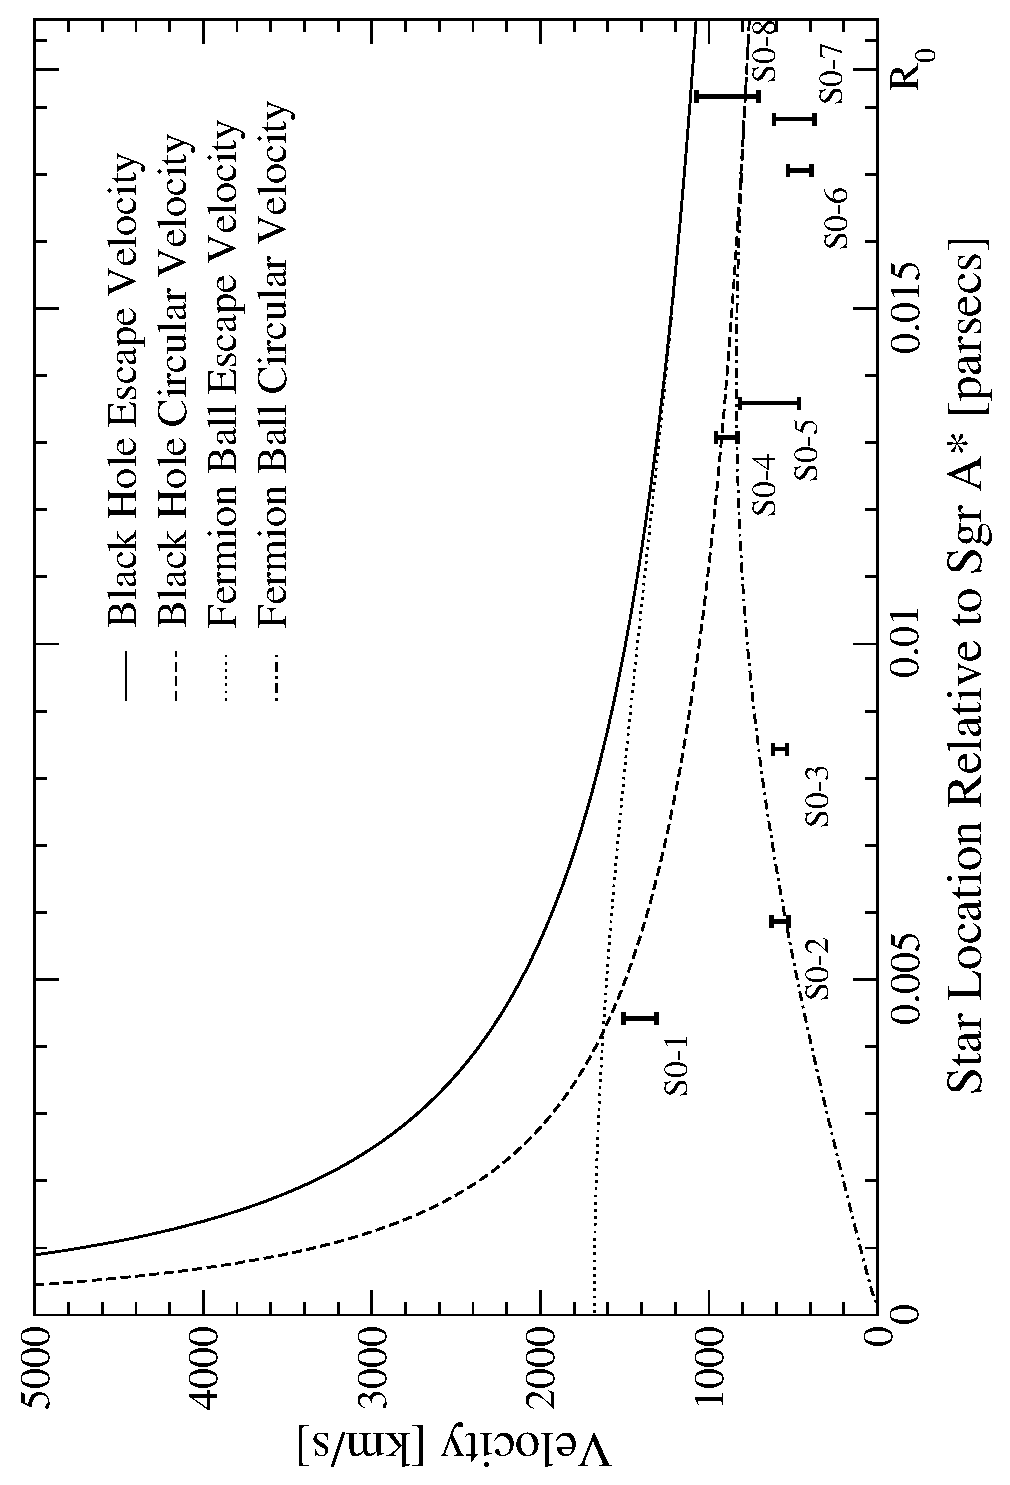
\includegraphics[angle=-90,width=0.9\textwidth]{eps/escapevelocitieswithdata.eps}
	\caption{Velocities from proper motion analysis \cite{ref_ghezmotion} alongside the calculated escape and circular
	velocities for the black hole and fermion ball scenarios. Fermion ball radius noted as ${\rm R_0}$.
	This plot is made using the position and velocity vectors as calculated from the right ascension and declination data. There
	is no data available in our line of sight, thus all points are minimal values. Epoch 1996.58.}
	\label{fig_escapevelocities}
	\end{center}
\end{figure}

S0-3 is suspected to have a very large position component in our line of sight (due to it's near `straight line' trajectory)
and is therefore ruled out as an object of interest.
However, from Figure \ref{fig_escapevelocities} it is clear that the stars S0-1 through S0-5 may be within the projected radius
of the fermion ball. However, of those stars, only S0-1, S0-2 and S0-4 have been identified as being on accelerating orbits.
We will therefore use these 3 stars to draw comparisons with models of motion.

\subsection{Newtonian Motion}
We calculate the trajectories of the stars by solving Newton's equations of motion in 3-dimensions
\begin{eqnarray}
	\frac{d^2x}{dt^2} = - \frac{G M(r)}{\left(x^2 + y^2 + z^2\right)^{\frac{3}{2}}}x \nonumber \\
	\frac{d^2y}{dt^2} = - \frac{G M(r)}{\left(x^2 + y^2 + z^2\right)^{\frac{3}{2}}}y
	\label{eqn_newtonmotion} \\
	\frac{d^2z}{dt^2} = - \frac{G M(r)}{\left(x^2 + y^2 + z^2\right)^{\frac{3}{2}}}z \nonumber
\end{eqnarray}
where $x$, $y$, $z$ are the distances from the origin in a Euclidean coordinate system centred on Sgr A*,
taking $x$ to be opposite the observed right ascension, $y$ as the observed declination, and $z$ to be the line of sight in the
direction of the sun.
The solution of the coupled differential equations (\ref{eqn_newtonmotion}) depends upon 7 initial conditions, which are the $x$, $y$, $z$
position and velocity components with the mass of the central object as the final parameter. We first minimise the fit to initial $x$, $y$
position and $v_x$, $v_y$ velocity parameters, then run a $\chi^2$ phase space analysis on the $z$ position and velocity parameters.
The effect of varying the central mass is briefly discussed afterwards using limits imposed by \cite{ref_ghezmotion}.

The data we choose to use consists of a combination of spatial analysis from 2 independent sources \cite{ref_ghezorbits, ref_eckartorbits}
on the 3 stars S0-1, S0-2 and S0-4 over the observing period 1992.7 to 2000.5. The location of Sgr A* moves over time (against the background),
fortunately the data has already considered this and all positions are relative to the location of Sgr A*. There are 36
data points for each star from 18 separate observations, which must be fitted. It is important to stress that the parameters already
mentioned as initial conditions are for the 1992.7 epoch, and cannot be directly compared, to say, the data in Figure
\ref{fig_escapevelocities}, which is the epoch 1996.58.

\subsection{$\chi^2$ Reduction of $z$ and $v_z$}

\subsubsection{Notes on $\chi^2$}
A $\chi^2$ analysis is the most commonly accepted method for comparing experimental data to a theoretical model, a smaller value
signals a better fit to the experiment. A $\chi^2_{ndf}$ ($\chi^2$ per number of degrees of freedom) is a more rigorous way to examine the fit
as it will also consider the number of data points used and the number of free variables in the theory. The form of the data in this
case is such that we must perform a separate $\chi^2$ fit for both the $x$ and $y$ observed data, each given by
\begin{eqnarray}
	\chi^2_x &=& \sum_{i=1}^{N} \frac{\left(x_i-\overline{x}(x,v_x,y,v_y,z,v_z,M)\right)^2}{\sigma^2_{x_{err}}}
	\label{eqn_chisquarex} \\
	\chi^2_y &=& \sum_{i=1}^{N} \frac{\left(y_i-\overline{y}(x,v_x,y,v_y,z,v_z,M)\right)^2}{\sigma^2_{y_{err}}}
	\label{eqn_chisquarey}
\end{eqnarray}
These $\chi^2$ values can safely be added linearly as the nature of $\chi^2$ is such that it need not be added in quadrature (as the
$\chi$ itself will already be added in quadrature). The total $\chi^2$, which is the quantity of interest can then be written as
\begin{equation}
	\chi^2 = \chi^2_x + \chi^2_y
	\label{chisquare}
\end{equation}
and the $\chi^2$ per number of degrees of freedom is
\begin{equation}
	\chi^2_{ndf} = \frac{\chi^2}{N-N_p}
	\label{chisquarendf}
\end{equation}
where $N=36$ and $N_p=7$.

Simulations of star dynamics were performed several times in order to minimise the $\chi^2$ for initial parameters $x$, $v_x$, $y$
and $v_y$, but by no means have the $\chi^2$ been fully reduced. Computing time restricted the iterations of the simulations to 4
passes, and further iterations would most certainly produce slightly smaller $\chi^2$.

The astronomical unit of arcsec has been preferred in the presentation of the results as this is the unit used during observations.
This unit system may appear unusual when referring to the $z$ axis which is in the observer's line of sight, but it can be thought
of as being equivalent to the distance projected at a fixed distance of 8kpc, as can the $x$ and $y$ axis.

\subsubsection{Best Fits}
\label{bestfits}
By first minimising the initial $x$ and $y$ position and velocity parameters, this allows for a $\chi^2_{ndf}$ phase space plot of the
unknown $z$ position and velocity parameters. Table \ref{tab_minimalzvzchisquare} lists the minimal $\chi^2_{ndf}$ for each
of the 3 stars in each scenario. Figures \ref{fig_so1BHphasespace} through \ref{fig_so4FBphasespace} are the phase space plots, using
colour as the 3rd dimension. In order to ensure a high resolution in the data representation, each plot is a result of 22,000 runs of
the simulation. There has been no interpolation performed on the images.

Table \ref{tab_minimalzvzchisquare} reveals that the fits for S0-1 have a much higher $\chi^2_{ndf}$ compared with S0-2 and S0-4.
This is due to inconsistencies within the experimental data. Figures \ref{fig_so1bestfits} through \ref{fig_so4bestfits} show the
$x$ and $y$ paths of the stars for each of the reduced $\chi^2_{ndf}$ scenarios. Extra paths are also shown for bound orbits,
where the minimum fit $\chi^2_{ndf}$ is an unbound orbit. These tables highlight the numerically minimal $\chi^2$ values for each plot,
but as can be seen clearly from figures \ref{fig_so1BHphasespace} through \ref{fig_so4FBphasespace}, the minimal $\chi^2$ is not always
well defined and the $z$, $v_z$ values may take on a much larger range only expressible in the plots.

The inconsistencies within the S0-1 data can be clearly seen in Figure
\ref{fig_so1bestfits}, possibly due to the discernment of `north' not agreeing between each of the data sources, resulting in a
`rotation' effect.

Similar fits were also obtained for the extremal masses of Sgr A*, with similar $z$ - $v_z$, $\chi^2_{ndf}$ phase space plots.
Tables \ref{tab_minimalzvzchisquareminmass} and \ref{tab_minimalzvzchisquaremaxmass} show the minimal $\chi^2_{ndf}$ fits.
The mass does not appear to affect either scenario greatly and is the parameter of least impact to the fit. Re-iteration
would again, certainly reduce the $\chi^2_{ndf}$ slightly.
\clearpage
\begin{figure}[!pt]
	\begin{center}
	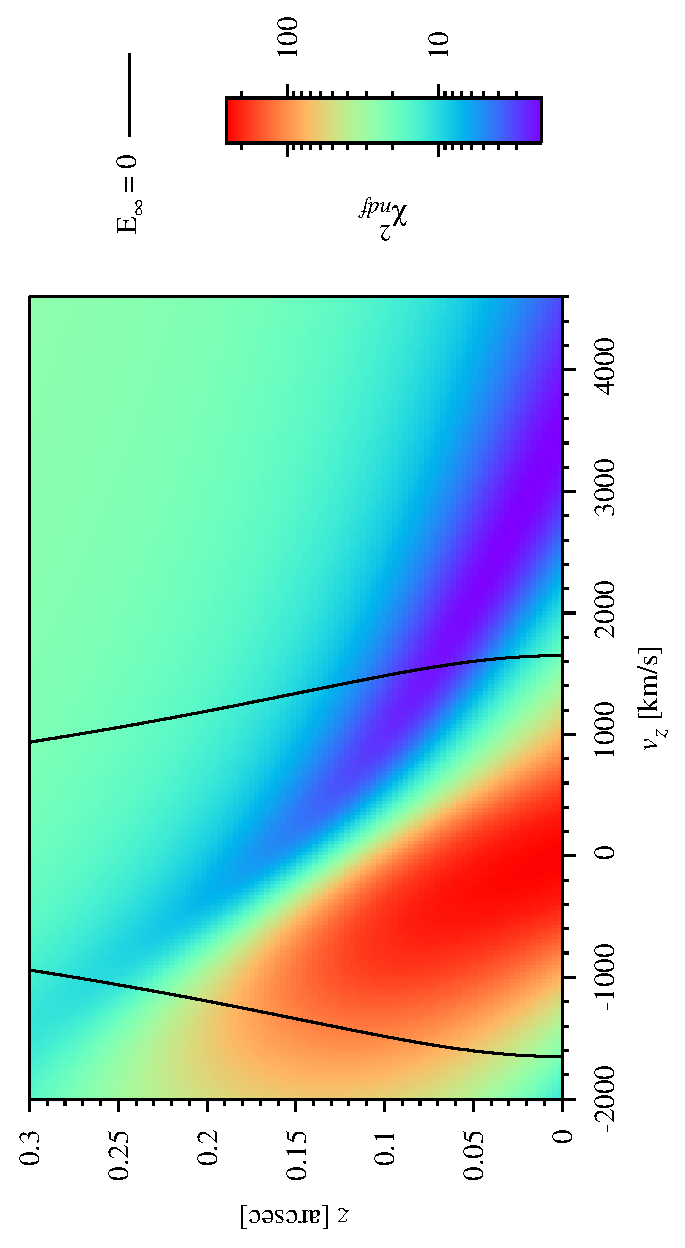
\includegraphics[angle=-90,width=0.9\textwidth]{eps/so1-BH-run3.eps}
	\caption{$\chi^2_{ndf}$ phase space plot for S0-1 with black hole. The lines represent the escape velocity required of the $v_z$
	component only, bound orbits being within the lines and unbound orbits outside. Epoch 1992.7.}
	\label{fig_so1BHphasespace}
	\end{center}
\end{figure}
\begin{figure}[!pb]
	\begin{center}
	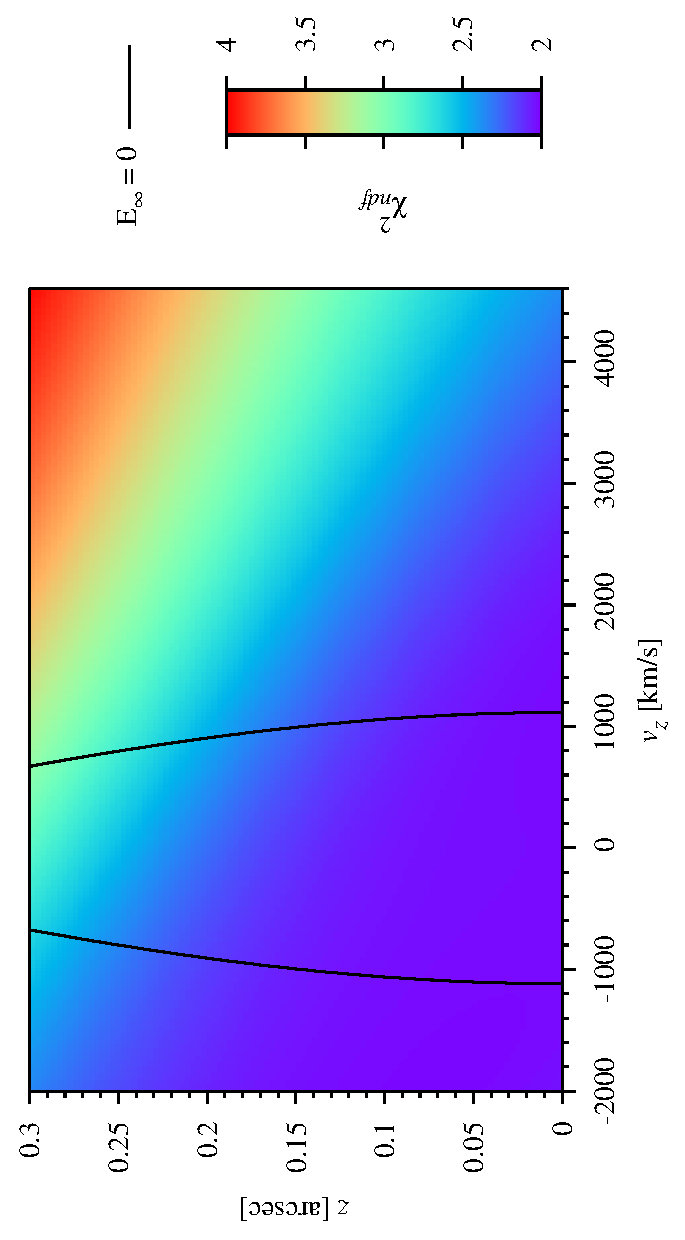
\includegraphics[angle=-90,width=0.9\textwidth]{eps/so1-FB-run9.eps}
	\caption{$\chi^2_{ndf}$ phase space plot for S0-1 with fermion ball. Epoch 1992.7.}
	\label{fig_so1FBphasespace}
	\end{center}
\end{figure}
\begin{figure}[!pt]
	\begin{center}
	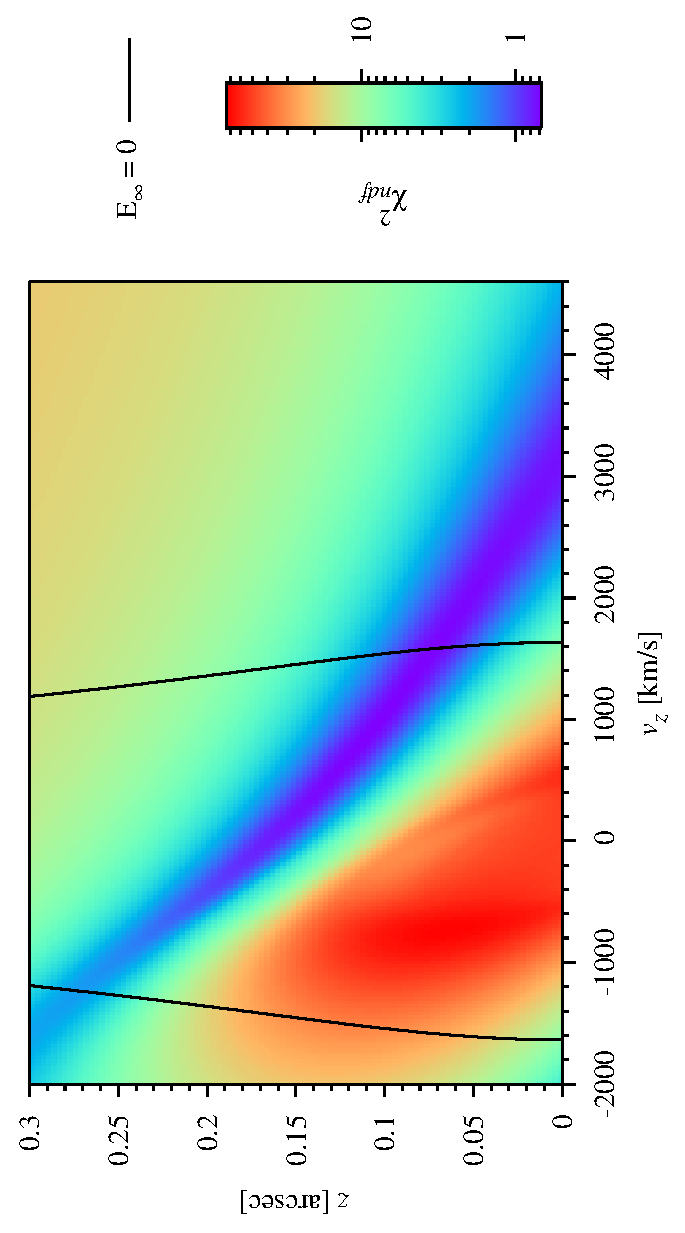
\includegraphics[angle=-90,width=0.9\textwidth]{eps/so2-BH-run2.eps}
	\caption{$\chi^2_{ndf}$ phase space plot for S0-2 with black hole. Epoch 1992.7.}
	\label{fig_so2BHphasespace}
	\end{center}
\end{figure}
\begin{figure}[!pb]
	\begin{center}
	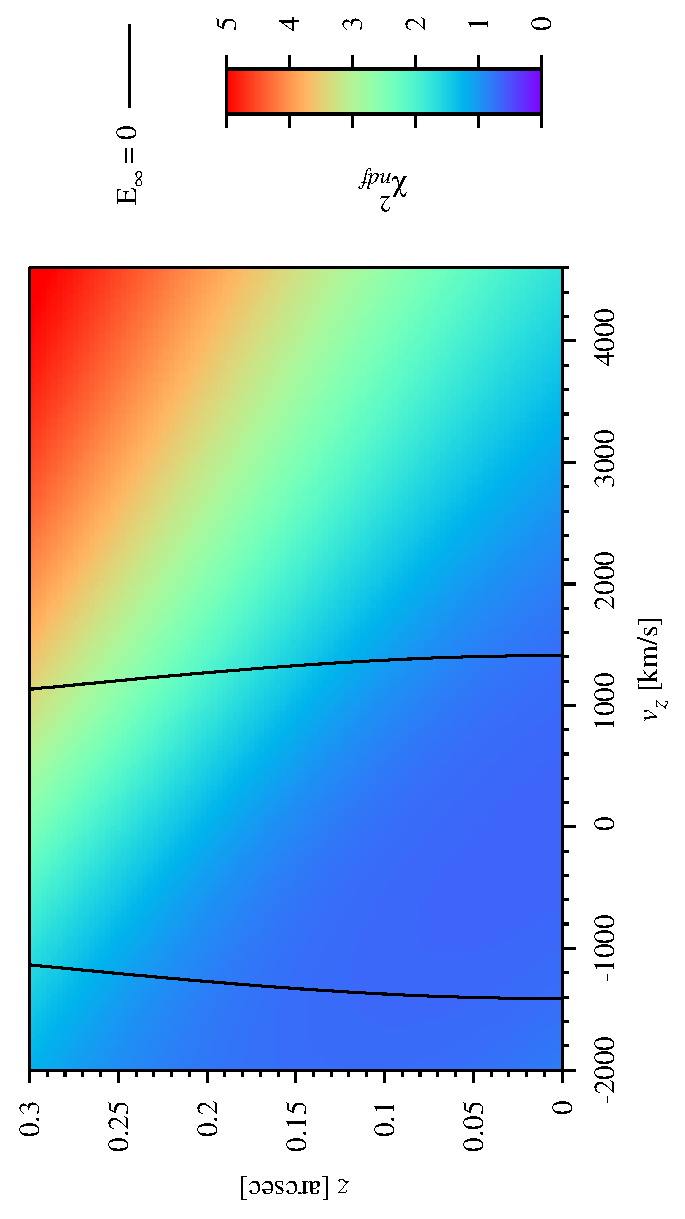
\includegraphics[angle=-90,width=0.9\textwidth]{eps/so2-FB-run9.eps}
	\caption{$\chi^2_{ndf}$ phase space plot for S0-2 with fermion ball. Epoch 1992.7.}
	\label{fig_so2FBphasespace}
	\end{center}
\end{figure}
\begin{figure}[!pt]
	\begin{center}
	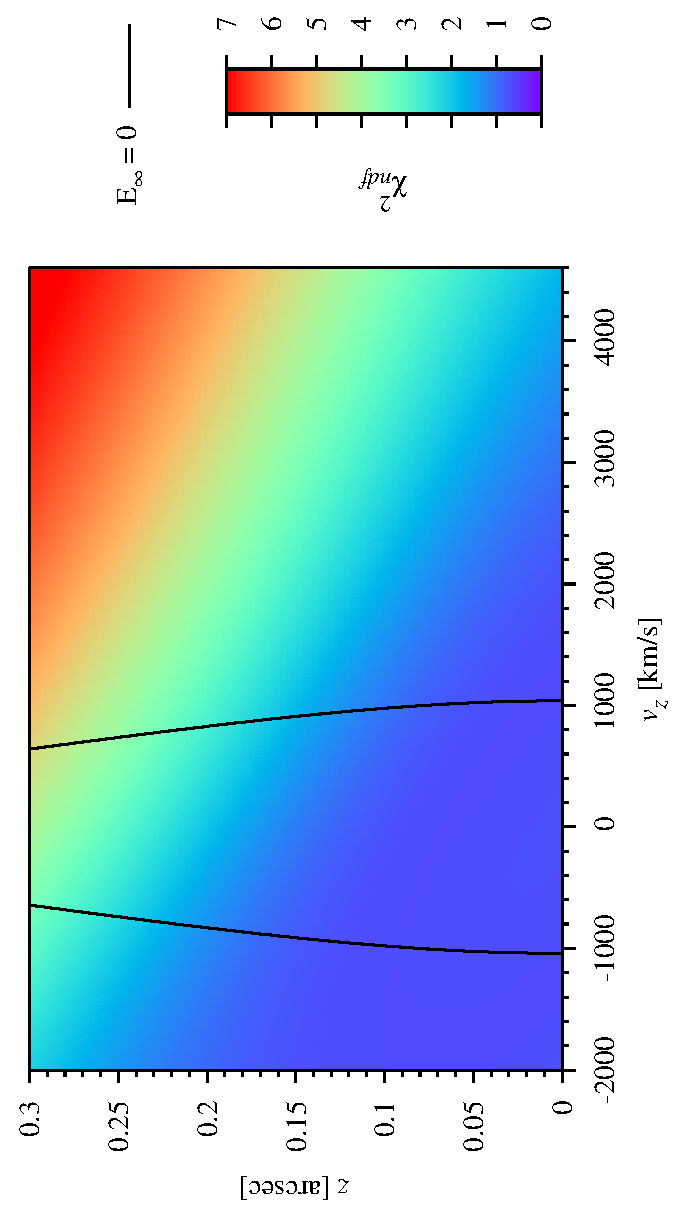
\includegraphics[angle=-90,width=0.9\textwidth]{eps/so4-BH-run2.eps}
	\caption{$\chi^2_{ndf}$ phase space plot for S0-4 with black hole. Epoch 1992.7.}
	\label{fig_so4BHphasespace}
	\end{center}
\end{figure}
\begin{figure}[!pt]
	\begin{center}
	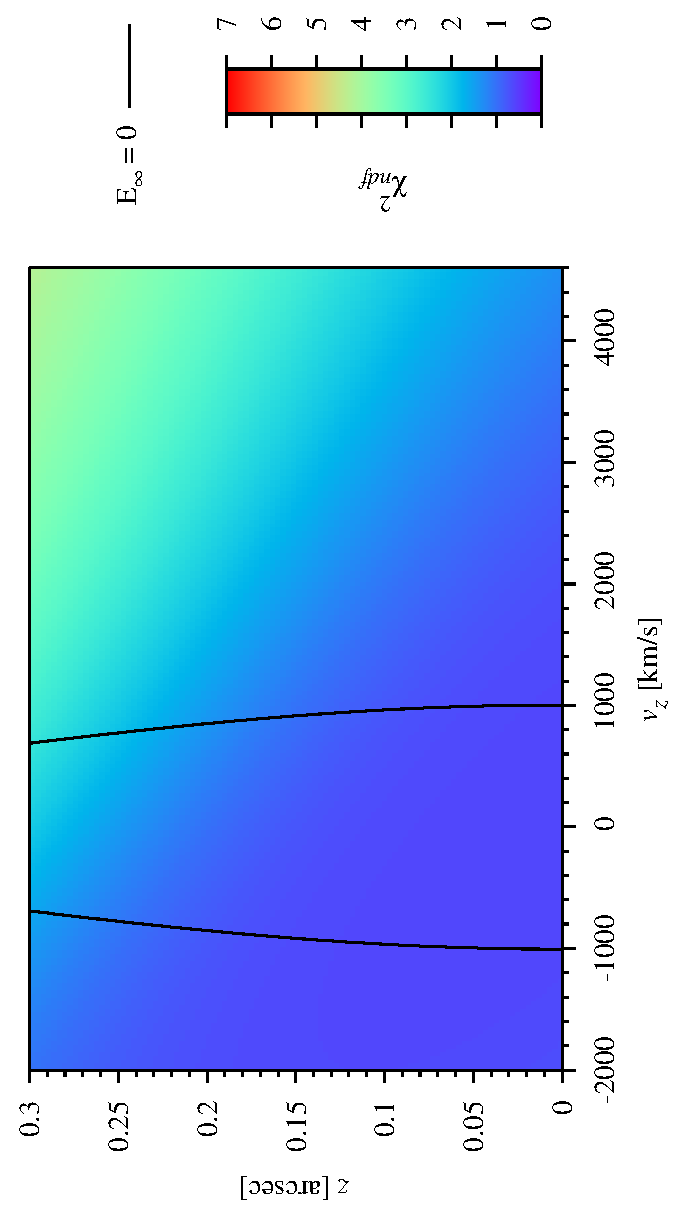
\includegraphics[angle=-90,width=0.9\textwidth]{eps/so4-FB-run9.eps}
	\caption{$\chi^2_{ndf}$ phase space plot for S0-4 with fermion ball. Epoch 1992.7.}
	\label{fig_so4FBphasespace}
	\end{center}
\end{figure}
\clearpage

\subsection{Analysis}
It is quite clear from Figures \ref{fig_so1BHphasespace} through \ref{fig_so4FBphasespace} that the fermion ball scenario applies 
much less constraints with selection of $z$ and $v_z$ initial conditions than the black hole scenario, which has quite rigid constraints.
Accurate
measurements of these parameters would most certainly be able to show if the black hole scenario describes the orbits sufficiently.
However, experimental complications in taking said measurements make this an unlikely method of discernment in the near future.

Due to the alikeness of Figures \ref{fig_so4BHphasespace} and \ref{fig_so4FBphasespace}, we can clearly see that phase space analysis on
S0-4 is unlikely to
be able to tell us much about the mass structure of the galactic centre. As the star would be located on the outer edge of the fermion ball,
the enclosed mass is almost that of the black hole, and the resulting dynamics are therefore very similar to those of the black hole scenario.
However, if S0-4 re-enters the fermion ball, a precessing orbit will be produced, and this will be observable over time. Also, it is
possible that S0-4 may travel incredibly close (within a milliparsec) of the black hole during the course of its orbit, for
Figure \ref{fig_so1bestfitssky} this occurs at around 2047. It may then be possible to observe relativistic effects upon
the star's spectra, assuming the technology to resolve these spectra will improve by that time. Obviously these effects would not be
present in the fermion ball scenario.

Observing the orbits of S0-1 and S0-2 will most certainly be a way to tell whether the galactic centre is a point source (black hole) or
an extended source. Unfortunately, the observations need to be made over a much longer timescale in order to see possible orbital precession.
S0-2 appears to show promise more quickly, allowing for discernment of any $z$-$v_z$ combination within a maximum of 30 years.
Data for $z$ and $v_z$ would certainly aid this process, and dramatically reduce the required observing time.
\begin{table}[!p]
	\begin{center}
	\begin{tabular}{c c c c c c c c c}
	\hline
	\hline
	Star & $x$ & $v_x$ & $y$ & $v_y$ & $z$ & $v_z$ & $\chi^2_{ndf}$ & Orbit \\
	\hline
	S0-1 BH &  0.125 & 0    & 0.105  & -900  & 0.012 & 3190  & 2.06 & unbound \\
	S0-1 FB &  0.121 & -200 & 0.110  & -1080 & 0.072 & -1940 & 2.02 & unbound \\
	S0-2 BH & -0.028 & 300  & 0.200  & -300  & 0.099 & 1090  & 0.68 & bound \\
	S0-2 FB & -0.028 & 300  & 0.200  & -450  & 0.000 & 40    & 0.65 & bound \\
	S0-4 BH & -0.250 & -800 & -0.120 & -600  & 0.000 & -1190 & 0.68 & unbound \\
	S0-4 FB & -0.250 & -760 & -0.116 & -600  & 0.072 & -410  & 0.65 & bound \\
	\hline
	\end{tabular}
	\end{center}
	\caption{Minimal $\chi^2_{ndf}$ for orbits of stars near the galactic centre. Final column notes a bound or unbound
	orbit using the escape velocity for that scenario, the number of degrees of freedom is 29. Positions 
	are in arcsec and velocities, km/s. All initial parameters are for epoch 1992.7 and for a mass of
	$2.6 \times 10^6 M_\odot$.}
	\label{tab_minimalzvzchisquare}
\end{table}
\begin{table}[!p]
	\begin{center}
	\begin{tabular}{c c c c c c c c c}
	\hline
	\hline
	Star & $x$ & $v_x$ & $y$ & $v_y$ & $z$ & $v_z$ & $\chi^2_{ndf}$ & Orbit \\
	\hline
	S0-1 BH &  0.125 & 0    & 0.105  & -900  & 0.000 & 3220  & 2.06 & unbound \\
	S0-1 FB &  0.121 & -200 & 0.110  & -1080 & 0.000 & 40    & 2.10 & bound \\
	S0-2 BH & -0.028 & 300  & 0.200  & -300  & 0.087 & 1120  & 0.68 & bound \\
	S0-2 FB & -0.028 & 300  & 0.200  & -450  & 0.000 & 40    & 0.83 & bound \\
	S0-4 BH & -0.250 & -800 & -0.120 & -600  & 0.000 & 40    & 0.69 & bound \\
	S0-4 FB & -0.250 & -760 & -0.116 & -600  & 0.000 & 40    & 0.70 & bound \\
	\hline
	\end{tabular}
	\end{center}
	\caption{Minimal $\chi^2_{ndf}$ for orbits of stars near the galactic centre of mass $2.4 \times 10^6 M_\odot$.}
	\label{tab_minimalzvzchisquareminmass}
\end{table}
\begin{table}[!p]
	\begin{center}
	\begin{tabular}{c c c c c c c c c}
	\hline
	\hline
	Star & $x$ & $v_x$ & $y$ & $v_y$ & $z$ & $v_z$ & $\chi^2_{ndf}$ & Orbit \\
	\hline
	S0-1 BH &  0.125 & 0    & 0.105  & -900  & 0.024 & 3130  & 2.07 & unbound \\
	S0-1 FB &  0.121 & -200 & 0.110  & -1080 & 0.000 & 2170  & 2.00 & unbound \\
	S0-2 BH & -0.028 & 300  & 0.200  & -300  & 0.111 & 1060  & 0.68 & bound \\
	S0-2 FB & -0.028 & 300  & 0.200  & -450  & 0.150 & -860  & 0.63 & bound \\
	S0-4 BH & -0.250 & -800 & -0.120 & -600  & 0.030 & 1450  & 0.68 & unbound \\
	S0-4 FB & -0.250 & -760 & -0.116 & -600  & 0.159 & -650  & 0.65 & bound \\
	\hline
	\end{tabular}
	\end{center}
	\caption{Minimal $\chi^2_{ndf}$ for orbits of stars near the galactic centre of mass $2.8 \times 10^6 M_\odot$.}
	\label{tab_minimalzvzchisquaremaxmass}
\end{table}
\begin{figure}[!p]
	\begin{center}
	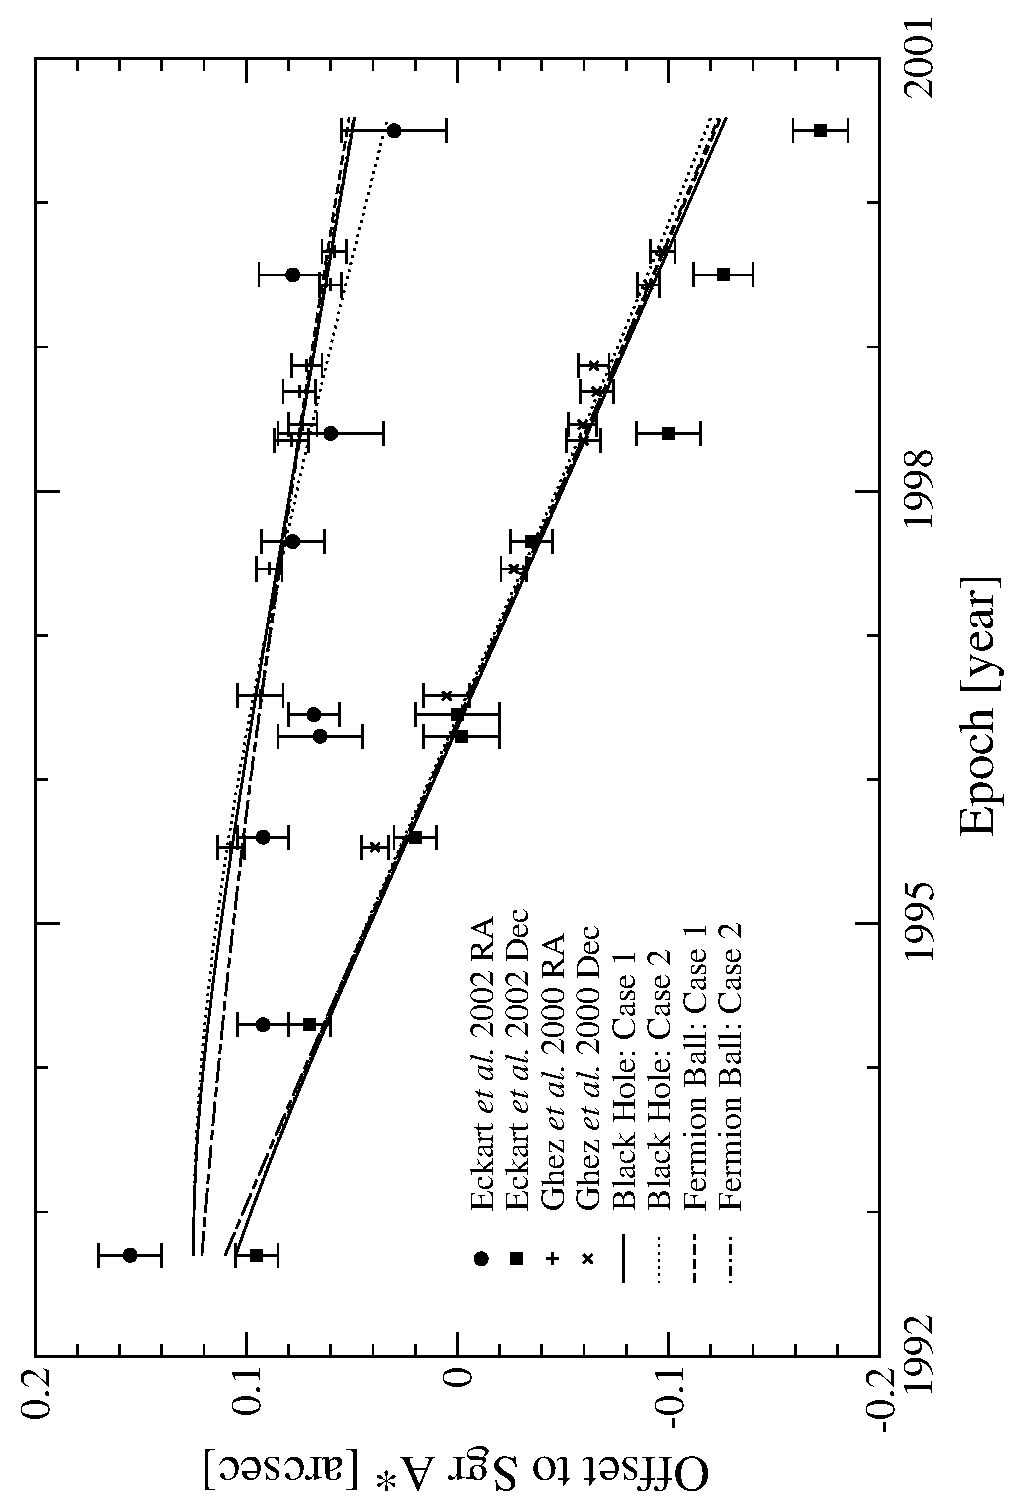
\includegraphics[angle=-90,width=0.9\textwidth]{eps/bestfits-so1.eps}
	\caption{Best fits for S0-1.
	``Black Hole: Case 1'' has $z$=0.012arcsec, $v_z$=3190km/s with an unbound orbit and $\chi^2_{ndf}=2.06$.
	``Black Hole: Case 2'' has $z$=0.075arcsec, $v_z$=1360km/s with a bound orbit and $\chi^2_{ndf}=2.54$.
	``Fermion Ball: Case 1'' has $z$=0.072arcsec, $v_z$=-1940km/s with an unbound orbit and $\chi^2_{ndf}=2.02$.
	``Fermion Ball: Case 2'' has $z$=0arcsec, $v_z$=0km/s with a bound orbit and $\chi^2_{ndf}=2.03$.}
	\label{fig_so1bestfits}
	\end{center}
\end{figure}
\begin{figure}[!p]
	\begin{center}
	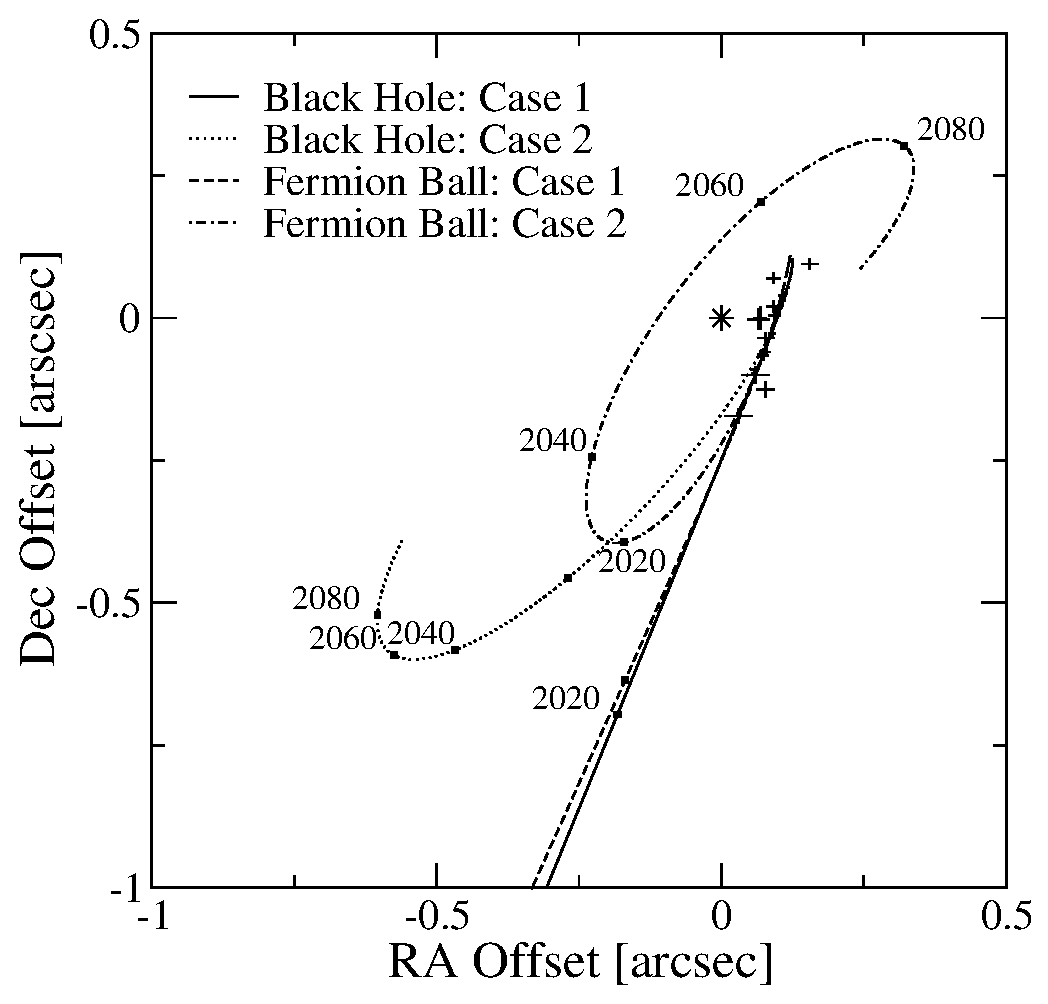
\includegraphics[width=0.9\textwidth]{eps/skyplot-so1.eps}
	\caption{Best fits for S0-1, sky-plot projected until 2100. All cases carry the same initial conditions as
	Figure \ref{fig_so1bestfits}. The dynamic location of Sgr A* is denoted by the star.}
	\label{fig_so1bestfitssky}
	\end{center}
\end{figure}
\begin{figure}[!p]
	\begin{center}
	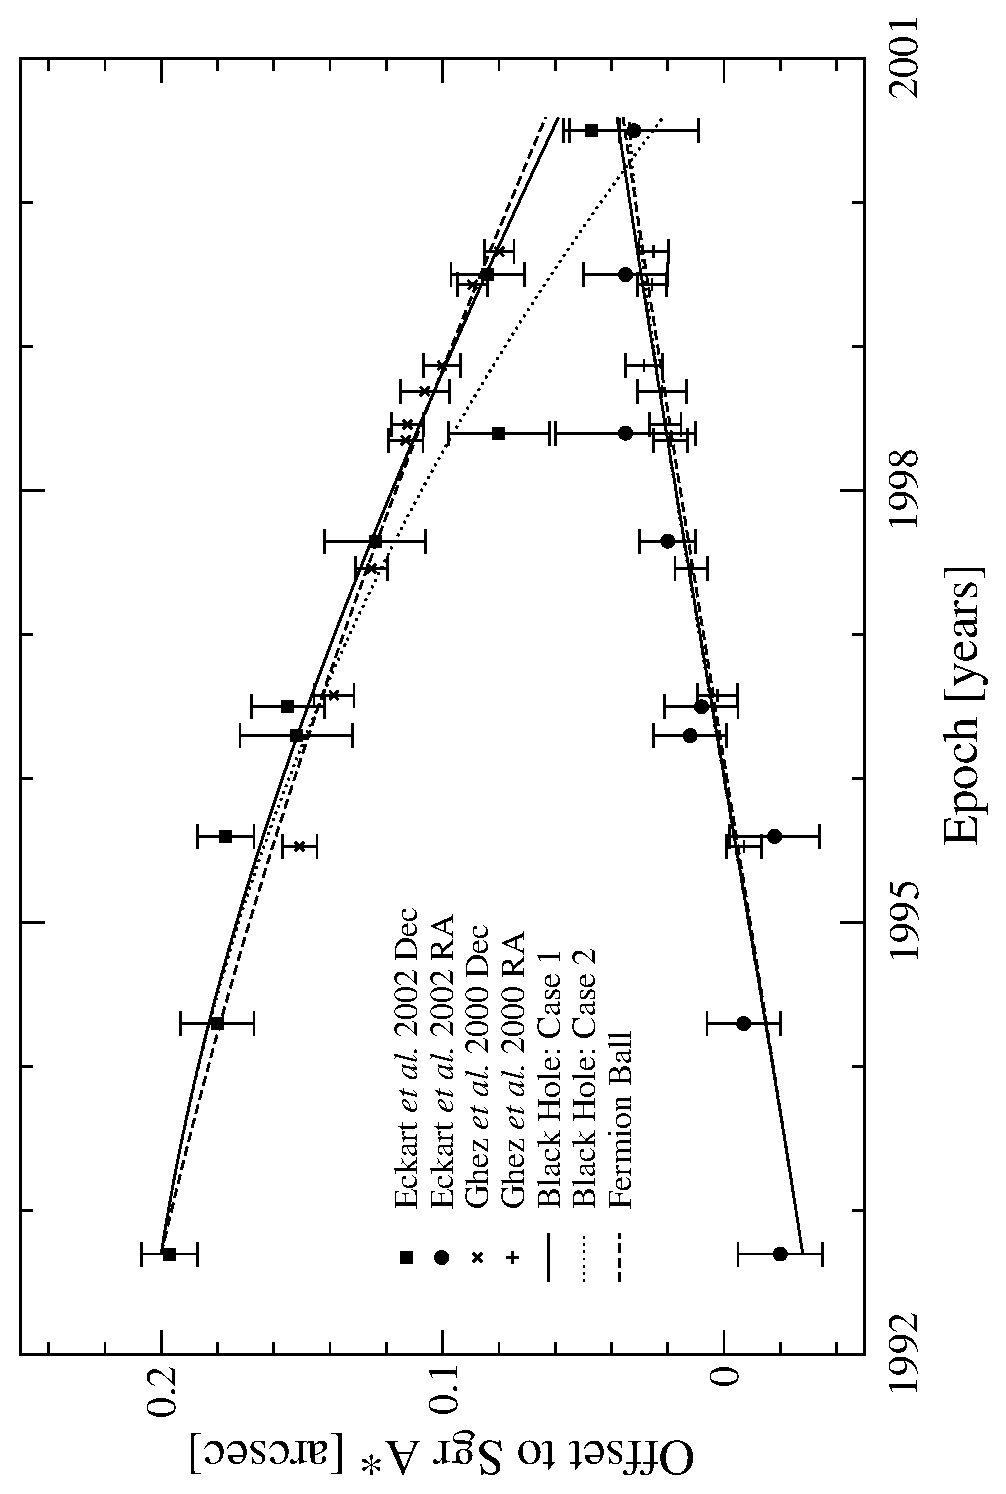
\includegraphics[angle=-90,width=0.9\textwidth]{eps/bestfits-so2.eps}
	\caption{Best fits for S0-2.
	``Black Hole: Case 1'' has $z$=0.099arcsec, $v_z$=1090km/s with a bound orbit and $\chi^2_{ndf}=0.68$.
	``Black Hole: Case 2'' has $z$=0.099arcsec, $v_z$=500km/s with a bound orbit and $\chi^2_{ndf}=3.27$.
	``Fermion Ball'' has $z$=0arcsec, $v_z$=40km/s with a bound orbit and $\chi^2_{ndf}=0.65$.
	``Black Hole: Case 2'' has been chosen in order to describe a very tight orbit around Sgr A*.}
	\label{fig_so2bestfits}
	\end{center}
\end{figure}
\begin{figure}[!p]
	\begin{center}
	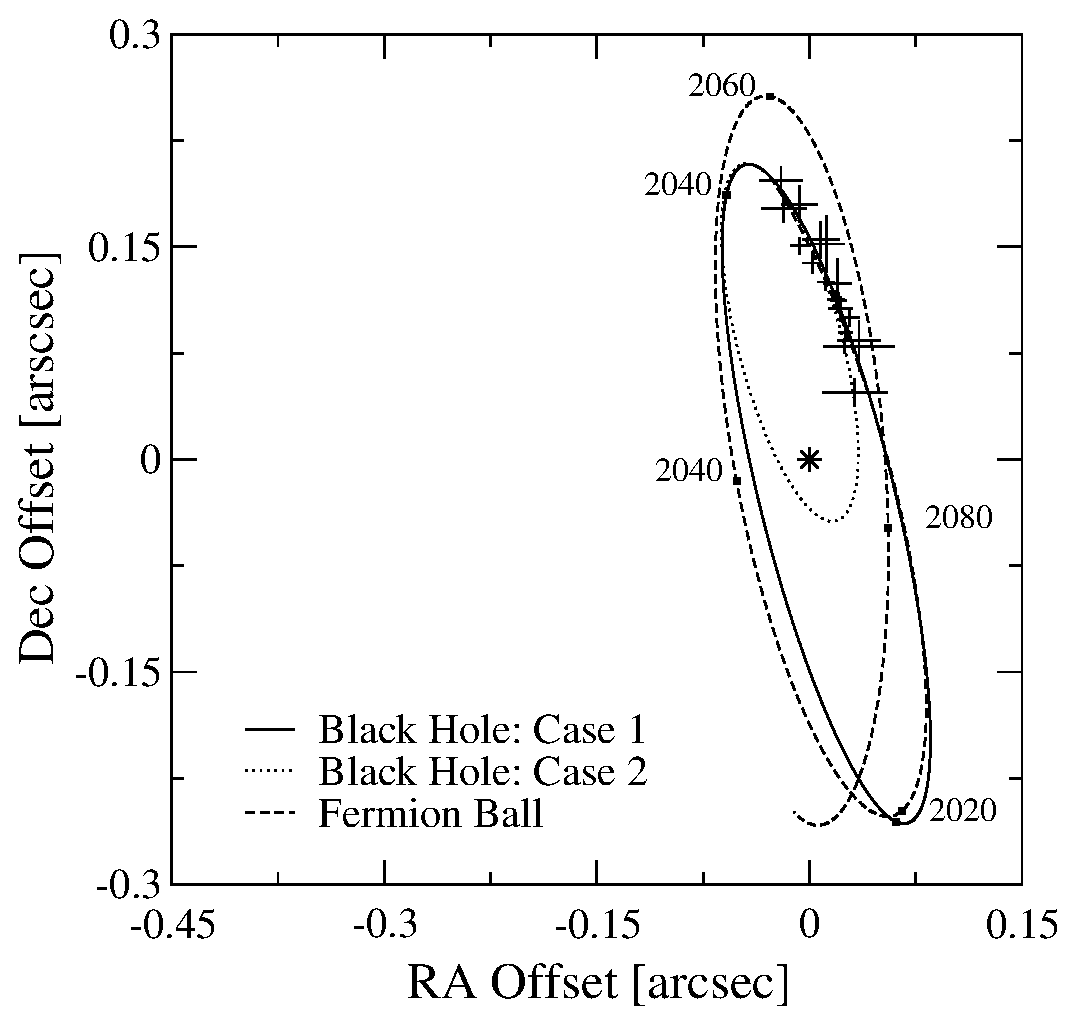
\includegraphics[width=0.9\textwidth]{eps/skyplot-so2.eps}
	\caption{Best fits for S0-2, sky-plot projected until 2100. All cases carry the same initial conditions as
	Figure \ref{fig_so2bestfits}. The black hole case 1 has a bound orbital period of 50 years, case 2 of 20 years.
	The dynamic location of Sgr A* is denoted by the star.}
	\label{fig_so2bestfitssky}
	\end{center}
\end{figure}
\begin{figure}[!p]
	\begin{center}
	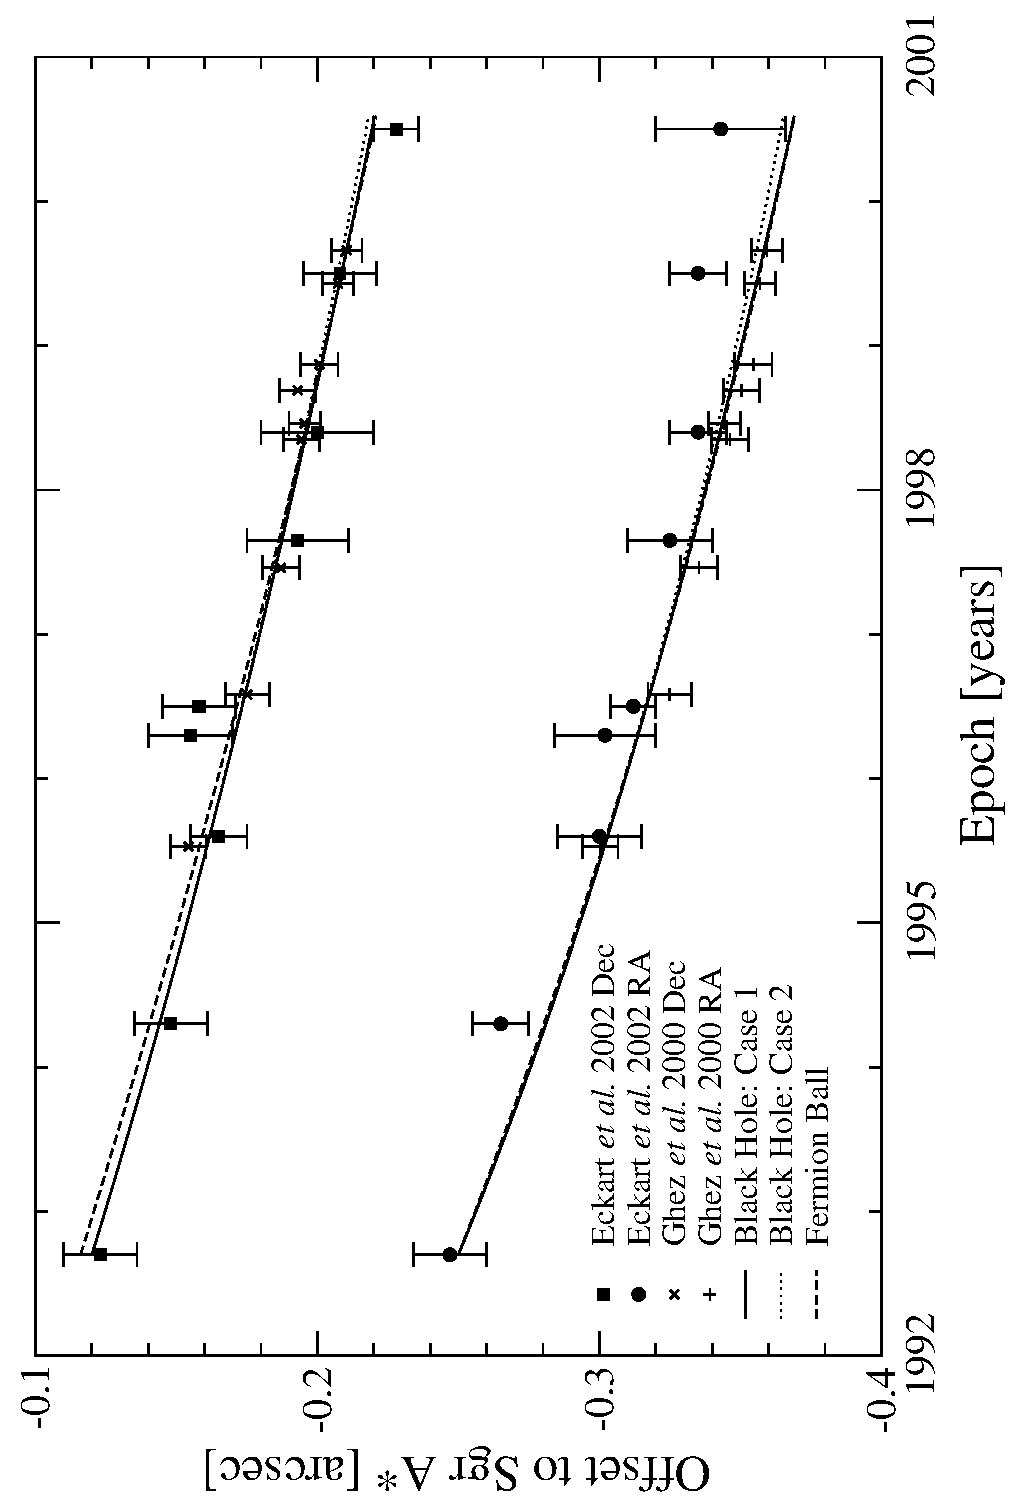
\includegraphics[angle=-90,width=0.9\textwidth]{eps/bestfits-so4.eps}
	\caption{Best fits for S0-4.
	``Black Hole: Case 1'' has $z$=0arcsec, $v_z$=-1190km/s with an unbound orbit and $\chi^2_{ndf}=0.68$.
	``Black Hole: Case 2'' has $z$=0arcsec, $v_z$=0km/s with a bound orbit of $\chi^2_{ndf}=0.72$.
	The ``Fermion Ball'' case has $z$=0.072arcsec, $v_z$=-410km/s with a bound orbit and $\chi^2_{ndf}=0.65$.}
	\label{fig_so4bestfits}
	\end{center}
\end{figure}
\begin{figure}[!p]
	\begin{center}
	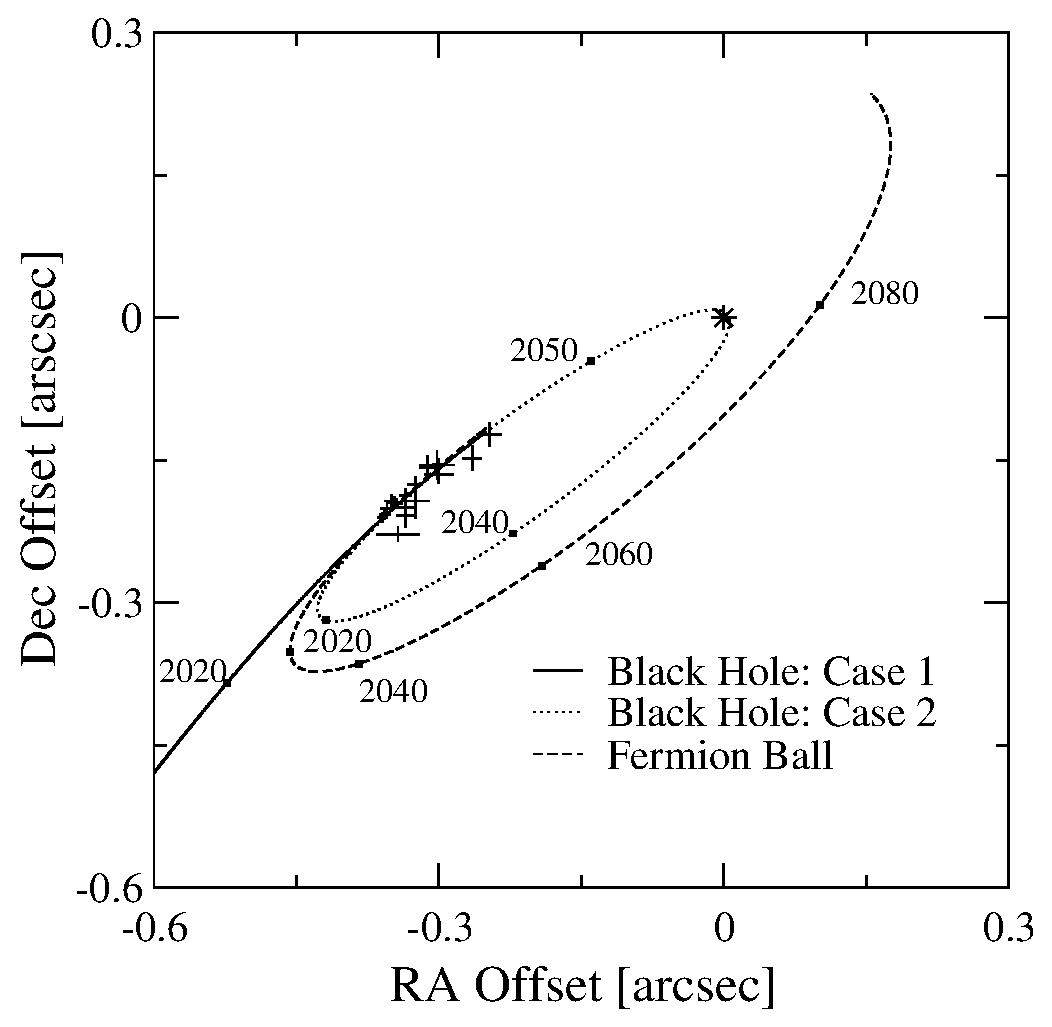
\includegraphics[width=0.9\textwidth]{eps/skyplot-so4.eps}
	\caption{Best fits for S0-4, sky-plot projected until 2100. All cases carry the same initial conditions as
	Figure \ref{fig_so4bestfits}. ``Black Hole: Case 2'' has a bound orbital period of 60 years. The dynamic
	location of Sgr A* is denoted by the star.}
	\label{fig_so4bestfitssky}
	\end{center}
\end{figure}
\clearpage

\subsection{The Importance of $v_z$ and $z$}
\label{sec_futureps}
Since Newton's equations of motion (\ref{eqn_newtonmotion}) are time reflection invariant, it is possible to numerically solve the
orbital paths back-wards in time.
This allows for setting of initial parameters in any epoch. If accurate $z$ or $v_z$ data were to be made available in say 2005,
it would constrain the $\chi^2$ phase space plots for that epoch, dramatically reducing the required observing time needed
for distinguishing black hole or mass distribution.

Several phase space plots are now presented for epoch 2005 (Figures \ref{fig_so1-2005-run2} and \ref{fig_so2-2005-run1}),
with initial parameters projected from the $\chi^2$ reduction in Section \ref{bestfits}.
However, data fitting is restricted to pre 2000.5 (the most recent observation) and we have therefore assumed
an orbital path up to our `initial' start date of 2005.

It is clear from these plots that accurate $z$ and $v_z$ would instantly allow distinguishing between the 2 scenarios.
\begin{figure}[!p]
	\begin{center}
	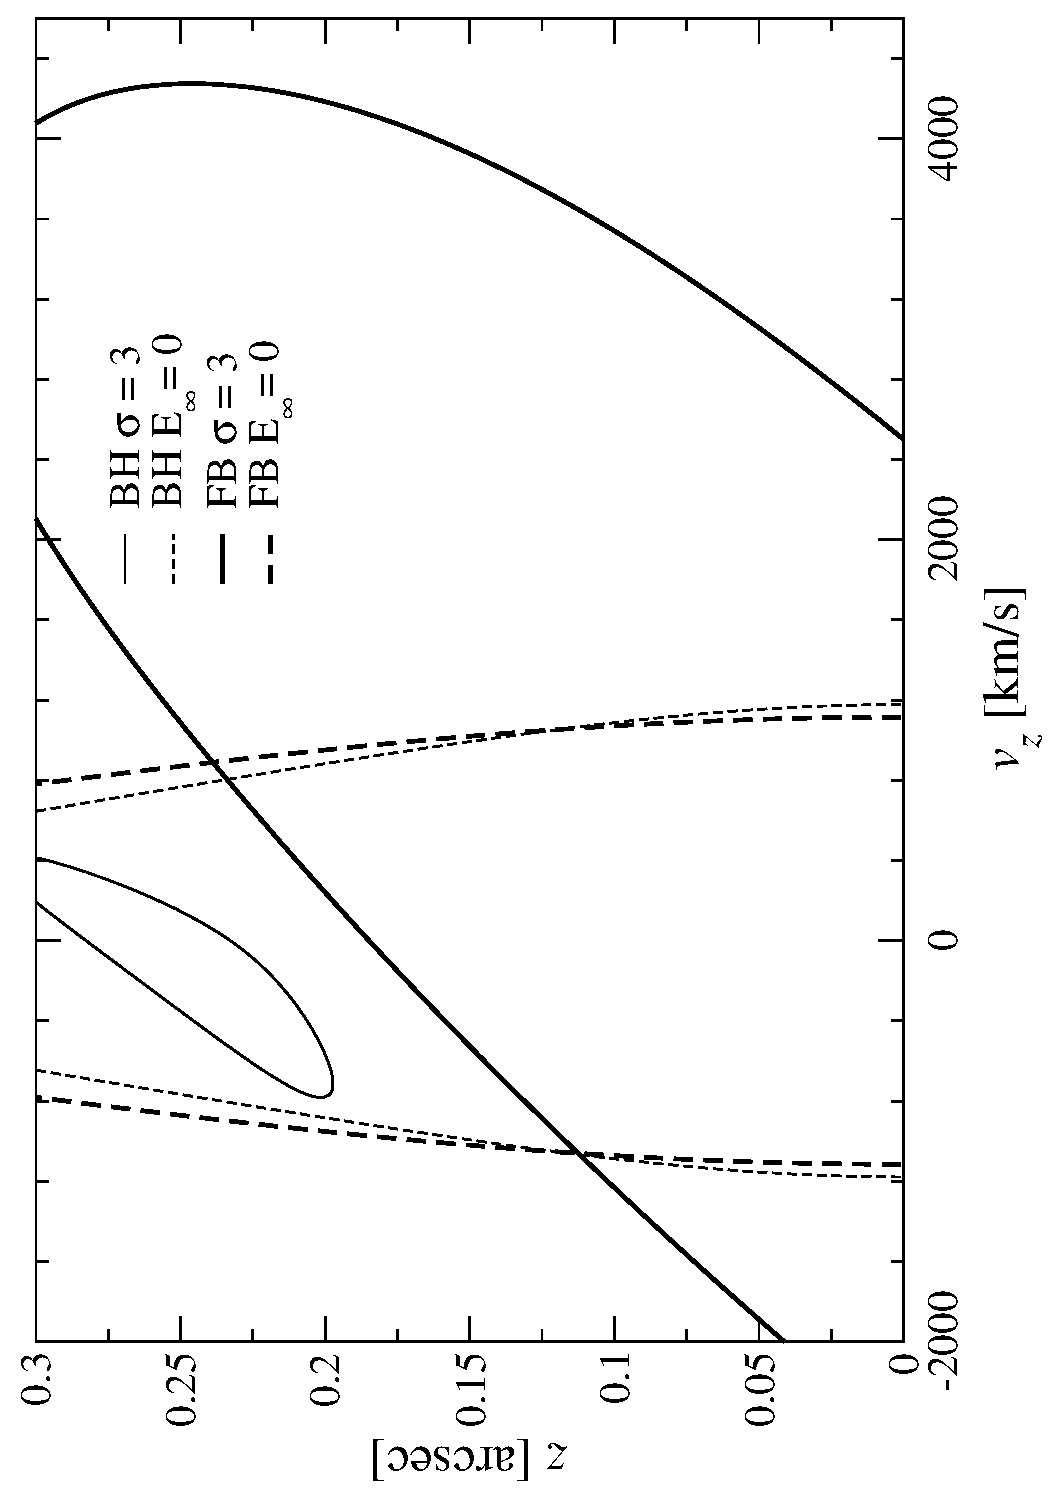
\includegraphics[angle=-90,width=0.9\textwidth]{eps/phasespace-2005-run2-so1.eps}
	\caption{$\chi^2_{ndf}$ phase space plot for S0-1 at epoch 2005. The paths for both ``Case 2'' scenarios in Figure
	\ref{fig_so1bestfits} have been used to give the `initial' position and velocity parameters for this plot (therefore we have
	assumed a bound orbit), values are in Table \ref{tab_so1-2005-run2}.
	Contour lines for $\chi^2_{ndf}$=3 are shown for both black hole and fermion ball scenarios, alongside
	the corresponding escape velocities.
	It is clear that the minimal $\chi^2_{ndf}$ values for each scenario occupy different regions
	and therefore an accurate measurement of $z$ or $v_z$ would instantly allow one of the scenarios to be eliminated. For example a
	$z$ measurement of 0.05arcsec would disallow the black hole scenario, similarly a $z$ measurement of 0.25arcsec and $v_z$
	of 0km/s would rule out the fermion ball scenario.}
	\label{fig_so1-2005-run2}
	\end{center}
\end{figure}
\begin{table}[!p]
	\begin{center}
	\begin{tabular}{c c c c c}
	\hline
	\hline
	Scenario & $x$ & $v_x$ & $y$ & $v_y$\\
	\hline
	BH &  -0.044 & -656  & -0.227 & -822 \\
	FB &  -0.007 & -492  & -0.233 & -811 \\
	\hline
	\end{tabular}
	\end{center}
	\caption{Initial parameters for Figure \ref{fig_so1-2005-run2}. Epoch 2005. Positions are in arcsec and velocities, km/s.}
	\label{tab_so1-2005-run2}
\end{table}
\clearpage
\begin{figure}[!p]
	\begin{center}
	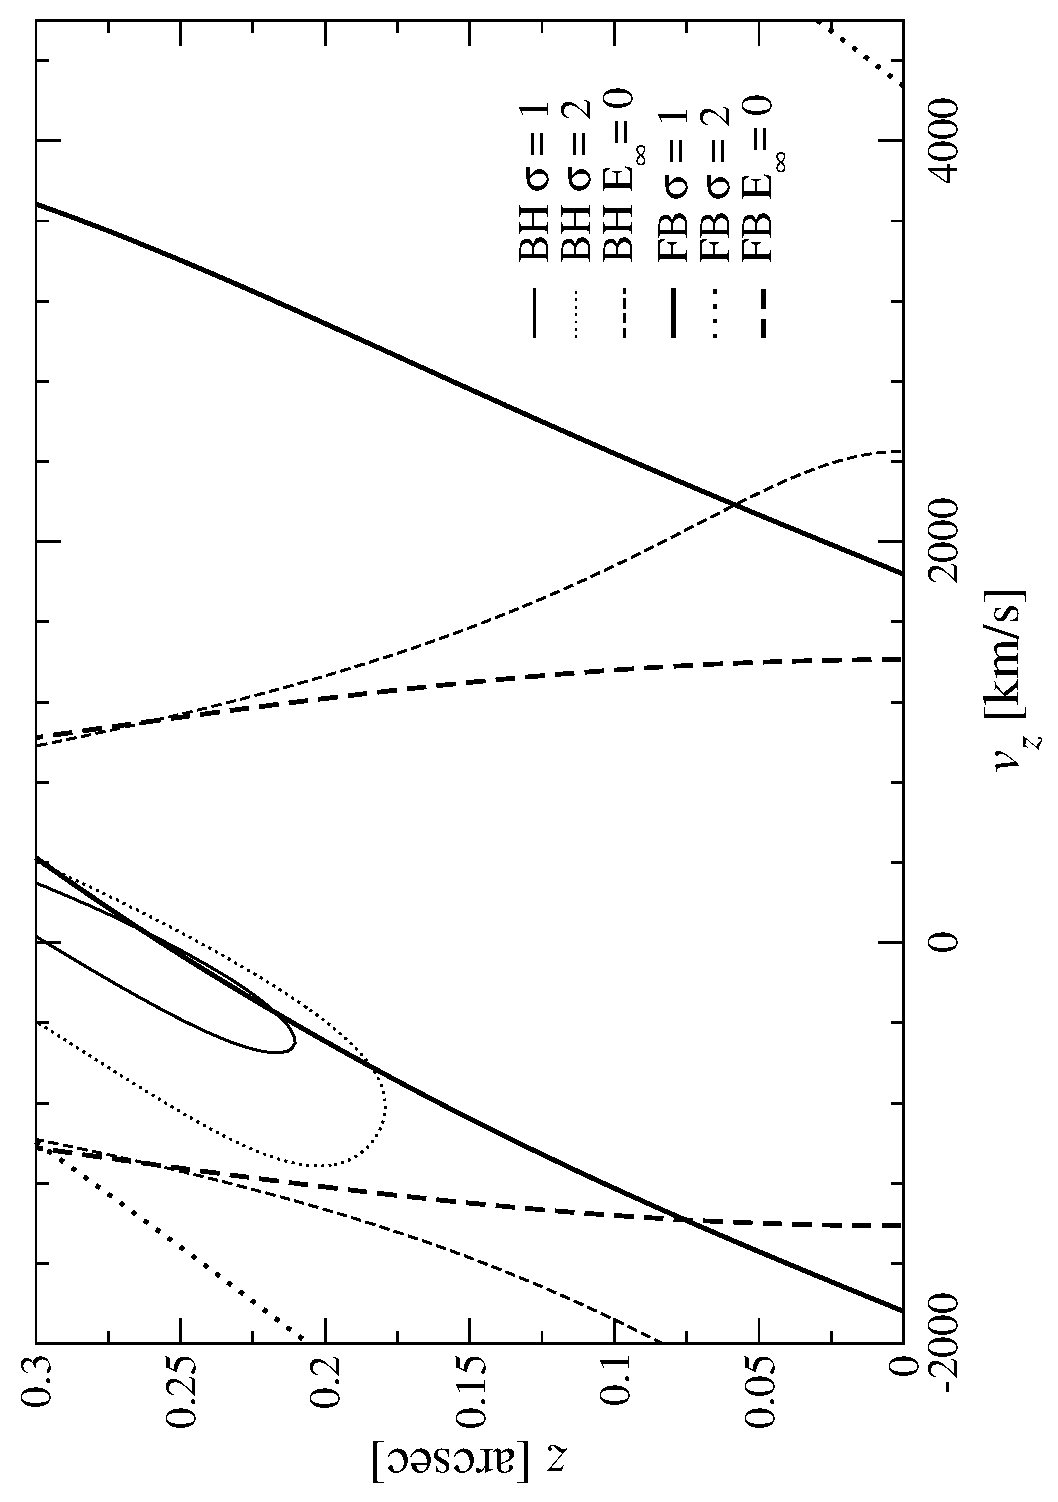
\includegraphics[angle=-90,width=0.9\textwidth]{eps/phasespace-2005-run1-so2.eps}
	\caption{$\chi^2_{ndf}$ phase space plot for S0-2 at epoch 2005. The minimal $\chi^2$ paths in Figure \ref{fig_so2bestfits}
	have been used to give the `initial' position and velocity parameters for this plot, values are in Table \ref{tab_so2-2005-run1}.
	Contour lines for $\chi^2_{ndf}$=1 and 2 are shown for both black hole and fermion ball scenarios, alongside the corresponding
	escape velocities.
	In this case, an accurate measurement of $z$ or $v_z$ may only allow for elimination of the black hole scenario, as the fermion ball
	minimal $\chi^2_{ndf}$ region is quite large.}
	\label{fig_so2-2005-run1}
	\end{center}
\end{figure}
\begin{table}[!p]
	\begin{center}
	\begin{tabular}{c c c c c}
	\hline
	\hline
	Scenario & $x$ & $v_x$ & $y$ & $v_y$\\
	\hline
	BH &  -0.067 & -196  & -0.050 & -922 \\
	FB &  -0.064 & -194  & -0.035 & -845 \\
	\hline
	\end{tabular}
	\end{center}
	\caption{Initial parameters for Figure \ref{fig_so2-2005-run1}. Epoch 2005. Positions are in arcsec and velocities, km/s.}
	\label{tab_so2-2005-run1}
\end{table}

\section{Spectrum by Accretion of Matter}
\label{sec_accretion}
\begin{quotation}
	\raggedleft \it
	Simulations are like miniskirts,\\
	they show a lot, but hide the essentials.\\
	-- Hubert Kirrmann
\end{quotation}
The observed spectrum of the object at the centre of our galaxy is quite unusual. The spectrum seems to have no emission in the infra-red (IR)
region, due to a very steep `cut-out' between $10^{12}$ and $10^{13}$Hz \cite{ref_meliareview}.
In this section, we investigate a very simple Newtonian accretion model \cite{ref_FKR},
which assumes that the accretion disk is both geometrically thin and optically thick (we will return to the non-validity of this assumption
later). We will show how a mass distribution, such as that of a fermion ball, will naturally produce this sudden drop in the accretion
spectrum.

\subsection{Source of the Accreting Gas}
Radio continuum observations have revealed a `cometary tail' of ionised gas from IRS7 (the brightest 2$\mu$m source in the central
parsec of the galaxy) leading away from the the location of Sgr A*. The tail appears to be formed by a `circumnuclear' wind which has been
observed originating from the cluster of stars IRS16 (which is an IR source close to, but not incident with Sgr A*) \cite{ref_yusefmorris}.
This collision is highly supersonic and creates a bow-shock within the gas flows \cite{ref_melia}, see Figure \ref{fig_irs7}.
This bow-shock dissipates most of the directed kinetic energy and heats the gas to $7 \times 10^6$K.

\begin{figure}[p]
	\begin{center}
	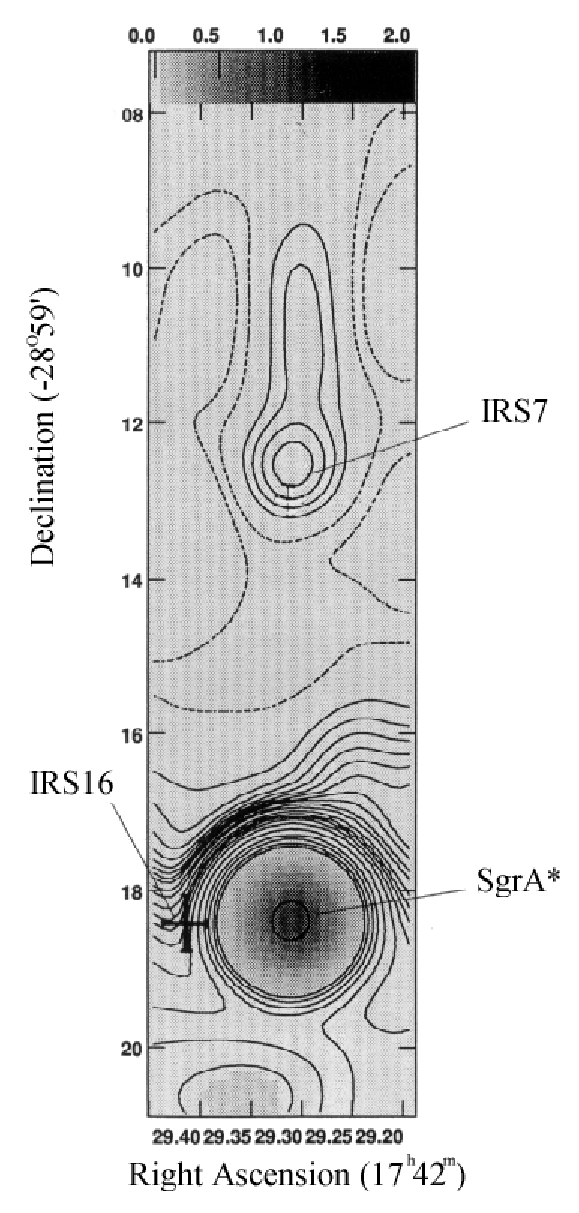
\includegraphics[angle=0,width=0.4\textwidth]{eps/irs7.eps}
	\caption{Contour map at $\lambda=2$cm of the IRS7 `cometary tail' with relation to Sgr A*. The tail is a result of the collision between
	the galactic centre and stellar winds rather than from the motion of IRS7 through the interstellar medium \cite{ref_yusefmorris}.}
	\label{fig_irs7}
	\end{center}
\end{figure}

Assuming that Sgr A* is not itself the source of the gaseous outflow, we may treat this gas as an excellent candidate for accretion
`fuel' in powering the spectrum, observed from the central object. We assume the shocked plasma falls in radially toward the central
object and that the accretion begins at radius $R_a$, given by the escape velocity
\begin{equation}
	R_a=\frac{2GM}{v_{gw}^2}
	\label{eqn_accretionstartradius}
\end{equation}
where $v_{gw}= 500 \rightarrow 700$ km/s. By simply comparing this velocity with Figure \ref{fig_escapevelocities}, we see that $R_a$
is significantly outside the fermion ball such that this equation will result the same for both scenarios. Although the limits of
accretion rate ($\dot{M}$) have been estimated in \cite{ref_melia} as $3 \rightarrow 40$ $\times 10^{-3}M_\odot$/yr,
is is widely accepted that the true values are much lower. The system
is therefore much below the Eddington-limited accretion rate and is called `weakly accreting'.
%\textcolor{red}{[I personally don't believe it is `much' below the Eddington-limited accretion rate!]}
We also take the most probable inclination angle of the accretion disk as $60^\circ$.

\subsection{Viscous Torque as a Means of Energy Release}
Consider 2 shearing `rings' in a gas of width $\lambda$, which meet at a surface of (radial) position $R$. Due to chaotic motions, gas
elements are constantly exchanged across this surface with speeds $\simeq \tilde v$. A typical element travels a distance $\lambda$ before
interacting on the other side of the surface.

These elements of fluid carry slightly different amounts of angular momentum, corresponding
to their location, either $R - \frac{\lambda}{2}$ or $R + \frac{\lambda}{2}$ (the substitutions $R_- = R - \frac{\lambda}{2}$ and
$R_+ = R + \frac{\lambda}{2}$ are made for clarity). This process cannot result in any net transfer of matter between the rings as
it occurs in equilibrium, therefore mass crosses the surface at equal rates in both directions of the order $\xi \widetilde{v}$ per unit
arc length, where $\xi$ is the surface density.

As the elements each possess separate angular momenta, there is a net transfer due to the chaotic processes, a `viscous torque' exerted
on the outer stream by the inner, et vice versa. The fluid at $R - \frac{\lambda}{2}$ will appear (to an observer moving with the rings)
to have velocity
\begin{equation}
	R_- \Omega (R_-) - R \Omega(R)
	\label{eqn_fluidvelocity1}
\end{equation}
and at $R + \frac{\lambda}{2}$
\begin{equation}
	R_+ \Omega (R_+) - R \Omega(R)
	\label{eqn_fluidvelocity2}
\end{equation}
Thus the average angular momentum `out' (i.e. from inner ring to outer) is (per unit arc length)
\begin{equation}
	R_- \widetilde{v} \xi \left[R_- \Omega (R_-) - R \Omega(R) \right]
	\label{eqn_fluidmomentumout}
\end{equation}
and `in'
\begin{equation}
	R_+ \widetilde{v} \xi \left[R_+ \Omega (R_+) - R \Omega(R) \right]
	\label{eqn_fluidmomentumin}
\end{equation}
Since mass flow is the same in each direction, the net flux of momentum (assuming chaotic motions occur on a much shorter timescale
than the angular velocity changes) can be written as
\begin{equation}
	\widetilde{v} \xi \left[ R_-^2 \Omega (R_-) - R_- R \Omega (R) - R_+^2 \Omega (R_+) + R_+ R \Omega (R) \right]
	\label{eqn_netflux}
\end{equation}
and to first order
\begin{eqnarray}
	&=& R^2 \widetilde{v} \xi \left[ \Omega(R_-) - \Omega(R_+) \right] \nonumber \\
	&=& R^2 \widetilde{v} \xi \lambda  \frac{d \Omega}{dr} \nonumber \\
	&=& \lambda  R^2 \widetilde{v} \xi \Omega '
	\label{eqn_netfluxfirstorder}
\end{eqnarray}
In an accretion disk, the rings are circular and we get the total torque by multiplying by the length $2 \pi R$. The torque exerted by the
outer ring on the inner is
\begin{equation}
	G(R) = 2 \pi R^3 v \xi \Omega '
	\label{eqn_torque}
\end{equation}
where the coefficient of viscosity is $v=\lambda \widetilde v$. Consider the net torque on a ring of gas between $R$ and $R+ \Delta R$.
As this has an inner and outer edge, it is subject to shearing from both sides. The net torque is
\begin{equation}
	G(R + dR) - G(R) = \frac{\partial G}{\partial R} dR
	\label{eqn_nettorqueofgas}
\end{equation}
Because the torque is a result of the angular velocity, there is a rate of work
\begin{equation}
	\Omega \frac{\partial G}{\partial R} dR = \left[ \frac{\partial (G \Omega)}{\partial R} - G \frac{\partial \Omega}{\partial R}\right] dR
	\label{eqn_nettorqueofgaswork}
\end{equation}
A simple summation will show that the first term (on the right hand side) is a rate of convection of rotational energy through the gas by the
torques. The second term represents a local rate of loss of mechanical energy to the gas. This `lost' energy must go into internal (heat)
energy. The viscous torques therefore cause dissipation within the gas at a rate $G \Omega ' dR$ per ring of width $dR$. Ultimately this
energy will be radiated over the upper and lower faces of the disk. We are therefore interested in the dissipation rate per unit plane
surface area, $D(R)$. Remembering that each ring has 2 plane faces and thus a plane area $4 \pi R dR$, we find
\begin{equation}
	D(R) = \frac{1}{2} R^2 v \xi \Omega'^2
	\label{eqn_dissipationrate}
\end{equation}

\subsection{The Accretion Process}
In standard non-relativistic accretion theory, it is first assumed that the accreting material has sufficient angular momentum to form a `disk'
which is confined closely enough to the orbital plane to be considered a 2D gas flow. This is the `thin disk approximation'. The matter moves
with maximal angular velocity
\begin{equation}
	\Omega = \frac{v_\phi}{R} \leq \sqrt{\frac{GM(R)}{R^3}}
	\label{eqn_maximalangular}
\end{equation}
The gas is assumed to possess a small radial drift velocity ($v_R$) in addition to the circular velocity ($v_\phi$). $v_R$ is negative near
the surface of a central object so that matter is being accreted. The disk is characterised by its surface density $\xi(R,t)$. We now write
the mass and angular momentum transport conservation equations.

An annulus of the disk material, lying between $R$ and $R+\Delta R$ has total mass $2 \pi R \Delta R \xi$ and total angular momentum
$2 \pi R^3 \Delta R \xi \Omega$. The rate of change of both of these quantities is given by the net flow from the neighbouring annuli.
Again, making the substitution $R_+ = R+\Delta R$ (for clarity), the rate of change of the mass is
\begin{eqnarray}
	\frac{\partial (2 \pi R \Delta R \xi)}{\partial t} &=& 2\pi \left[Rv_R(R,t)\xi(R,t)-R_+v_R(R_+,t)\xi(R_+,t)\right] \nonumber \\
	&=& -2\pi \Delta R\frac{\partial(Rv_R\xi)}{\partial R}
	\label{eqn_changeofmass}
\end{eqnarray}
In the $R\rightarrow 0$ limit we get
\begin{equation}
	R\frac{\partial \xi}{\partial t}+\frac{\partial (Rv_R\xi)}{\partial R} = 0
	\label{eqn_changeofmasstolimit}
\end{equation}
If we take a steady disk structure (i.e. $\frac{\partial}{\partial t}\rightarrow 0$) then (\ref{eqn_changeofmasstolimit}) can be simplified
somewhat to
\begin{equation}
	Rv_R\xi={\rm constant}
	\label{eqn_changeofmasstolimitsimplified}
\end{equation}
As this is an integral of the mass conservation equation, it represents the constant inflow of mass through each point of the disk. We define
the accretion rate as
\begin{equation}
	\dot M=-2\pi Rv_R\xi
	\label{eqn_accretionrate}
\end{equation}
which is constant for all $R$ and has the units of kg/s or often $M_\odot$/yr. For conservation of momentum, we must include the
transport due to the net effects of the viscous torques $G(R,t)$. The rate of change of angular momentum is given by
\begin{eqnarray}
	\frac{\partial (2 \pi R^3 \Delta R \xi \Omega)}{\partial t} &=& 2\pi R^3v_R(R,t)\xi(R,t)\Omega(R) \nonumber \\
	&=& -2\pi \Delta R \frac{\partial (R^3v_R\xi \Omega)}{\partial R} + \frac{\partial G}{\partial R} \Delta R
	\label{eqn_changeofmomentum}
\end{eqnarray}
In the limit $\Delta R \rightarrow 0$ we obtain
\begin{equation}
	R\frac{\partial (R^2\xi \Omega)}{\partial t} + \frac{\partial (R^3v_R\xi \Omega)}{\partial R} = \frac{1}{2\pi}\frac{\partial G}{\partial R}
	\label{eqn_changeofmomentumtolimit}
\end{equation}
and for a steady disk
\begin{equation}
	R^3v_R\xi \Omega = \frac{1}{2\pi}(G+C)
	\label{eqn_accretion4}
\end{equation}
where $C$ is a constant of integration.

\subsubsection{Dissipation Rate for a Black Hole}
For the angular velocity (\ref{eqn_maximalangular}), we may assume Keplerian motion
\begin{equation}
	\Omega = \sqrt{\frac{GM}{R^3}}
	\label{eqn_kepler}
\end{equation}
The angular velocity of the disk material remains Keplerian, increasing inward, until it begins to decrease at a `boundary layer' of radial
extent $b$. Here there exists a radius $R=R_\star + b$, at which $\Omega '=0$. If $b \ll R_\star$, then $\Omega$ is very close to it's
Keplerian value. Using (\ref{eqn_torque}) in (\ref{eqn_accretion4})
\begin{equation}
	R^3\xi v_R \Omega = R^3v_R\xi \Omega ' +\frac{C}{2\pi}
	\label{eqn_accretion5}
\end{equation}
with $R=R_\star$, $\Omega '=0$ and using (\ref{eqn_accretionrate}) we have
\begin{equation}
	C=- \dot M \sqrt{GMR_\star}
	\label{eqn_solnofc}
\end{equation}
Substituting this back into (\ref{eqn_accretion5})
\begin{equation}
	v_R\xi = \frac{\dot M}{3\pi}\left[1-\sqrt{\frac{R_\star}{R}} \right]
	\label{eqn_accretion5withsolnofc}
\end{equation}
and using (\ref{eqn_dissipationrate}) we arrive at
\begin{equation}
	D(R)=\frac{3GM\dot M}{8\pi R^3}\left[1-\sqrt{\frac{R_\star}{R}} \right]
	\label{eqn_dissipationratebh}
\end{equation}
The event horizon of a black hole is at radius
\begin{equation}
	R_{schw}=\frac{2GM}{c^2}
	\label{eqn_blackholeeventhorizon}
\end{equation}
For $R \gg R_{schw}$ the potential describing the orbits is Keplerian, however, at radii around a few $R_{schw}$, the effects of general
relativity become important and matter is removed from its orbit by instabilities as fast as it arrives. It therefore has very little
time to radiate before it disappears. Thus the maximum energy per unit area which can be extracted by this sort of accretion is the
specific binding energy of the innermost stable orbit.

This all makes the black hole scenario much easier to study as there is no boundary layer as previously described for accretion onto stars.
The boundary condition is that $G(R)$ vanishes at $R_\star \sim 3R_{schw}$. So, the dissipation for a black hole can be written, for any $R$
as
\begin{equation}
	D(R)=\frac{3GM\dot M}{8\pi R^3}\left[1-\sqrt{\frac{3R_{schw}}{R}} \right]
	\label{eqn_dissipationbh}
\end{equation}

\subsubsection{Dissipation Rate for a Fermion Ball}
We cannot assume Keplerian motion inside the fermion ball, we must instead use
\begin{equation}
	\Omega \leq \sqrt{\frac{GM(R)}{R^3}} = \sqrt{\frac{Gd_\nu}{b_\nu^3}} \sqrt{\frac{\mu(x)}{x^3}}
	\label{eqn_nonkeplerian}
\end{equation}
where these are the dimensionless values used in Section \ref{sec_relatmassdist}, Equation (\ref{eqn_relatmassdistunits}). In
(\ref{eqn_accretion5}), we take the point where $\Omega '=0$ (i.e. maximal $\Omega$) which naturally occurs at the centre of the fermion
ball, and this simplifies things greatly. However, we will still keep the formalism to be as general as possible, and consider the case
where the maximal $\Omega_A$ occurs at a radius $R_A$. We will later set $R_A=0$. This gives a solution for $C$
\begin{equation}
	C=2\pi R_A^3 v_A \xi \Omega_A
	\label{eqn_solnofcfermion}
\end{equation}
which gives
\begin{equation}
	v_R\xi = \frac{v_R\xi \Omega}{\Omega '} - \frac{R_A^3 v_A \xi \Omega_A}{R^3 \Omega '}
	\label{eqn_accretion5withsolnofcfermion}
\end{equation}
Using (\ref{eqn_accretionrate})
\begin{equation}
	v\xi = -\frac{\dot{M}\Omega}{2\pi R \Omega '} + \frac{\dot{M}R_A^2\Omega_A}{2\pi R^3\Omega '}
	\label{eqn_dissipationarb1}
\end{equation}
and inserting into (\ref{eqn_dissipationrate}) we get
\begin{eqnarray}
	D(R)&=&-\frac{\dot{M}}{4\pi}\left(R\Omega \Omega ' - \frac{R_A^2 \Omega_A \Omega '}{R}\right) \nonumber \\
	&=&\frac{\dot{M}R\Omega \Omega '}{4\pi} \left[\frac{\Omega_A}{\Omega} \left(\frac{R_A}{R}\right)^2-1\right]
	\label{eqn_dissipationfb}
\end{eqnarray}
Note that there is no `inner radius' or `boundary layer' for the fermion ball scenario, and thus the gas is deposited in the centre.
This makes for an excellent star `breeding ground' at the location of Sgr A*, with an average star birth rate depending upon the mass
loss rate $\dot{M}$.

\subsection{Temperature Distribution Due to Accretion}
Using the Stefan-Boltzmann law to show the effective temperature from the dissipation rate (assuming instant radiation of the gravitational
binding energy)
\begin{equation}
	D(R)=\sigma T_{{\rm {\it eff}}}^4(R)
	\label{eqn_stefanboltzman}
\end{equation}

\subsubsection{Black Hole}
The black hole case is trivial. From (\ref{eqn_dissipationbh})
\begin{equation}
	T_{{\rm {\it eff}}}(R)=\left(\frac{3GM\dot{M}}{8\pi R^3\sigma}\right)^{\frac{1}{4}}\left[1-\sqrt{\frac{3R_{schw}}{R}}\right]^{\frac{1}{4}}
	\label{eqn_blackholeeffectivetemp}
\end{equation}

\subsubsection{Fermion Ball}
\label{sec_fermionballtempdist}
The fermion ball case is, unfortunately, much more tedious. From (\ref{eqn_dissipationfb}) we arrive at
\begin{equation}
	T_{{\rm {\it eff}}}(R)=\frac{\dot{M}Gd_\nu}{4\pi \sigma b_\nu^3}x\sqrt{\frac{\mu(x)}{x^3}}\frac{d}{dx}\sqrt{\frac{\mu(x)}{x^3}}
		\left[\frac{\Omega_A}{\Omega}\left(\frac{x_A}{x}\right)^2-1\right]
	\label{eqn_fbeffectivetemp}
\end{equation}
The reduction of the central part of this equation is documented in Appendix \ref{app_solnoffermiontempdist}, which allows us to write
the effective temperature distribution as
\begin{equation}
	T_{{\rm {\it eff}}}(R)=\left(\frac{\dot{M}Gd_\nu}{8\pi \sigma b_\nu^3}\right)^{\frac{1}{4}}
		   \left(\frac{x\mu '(x)-3\mu(x)}{x^3}\right)^{\frac{1}{4}}
		   \left[\frac{\Omega_A}{\Omega} \left(\frac{R_A}{R}\right)^2-1\right]^{\frac{1}{4}}
	\label{eqn_fermioneffectivetemp}
\end{equation}
This may be solved numerically using the mass distribution solution given in Section \ref{sec_relatmassdist}, Equations
(\ref{eqn_relativisticxsolution}) and (\ref{eqn_relativisticmusolution}).

\subsection{A Toy Model}
Although it has been previously mentioned that the gas from the bow-shock is heated to a temperature of $7 \times 10^6$K, the
cooling timescale is in the region of $10^5$ years. The standard model of accretion was developed in order to explain the
accretion of cool gas which has not been shocked by colliding winds. The cold temperature and high density of the accreting gas
allows it to settle into an optically thick, geometrically thin disk. Neither of these conditions hold for the centre of the
Milky Way. As this is however, a much simpler model to investigate, we make the optically thick, geometrically thin approximation.
More complicated Advection Dominated Accretion Flow models have been developed \cite{ref_rees, ref_narayan}, and are much more successful
at describing the observed spectrum emanating from the centre of the Milky Way for a black hole scenario.

\subsubsection{The Optically Thick Approximation}
We make the assumption that the gas is optically thick, so we may treat it as a black body radiator, although Appendix
\ref{app_opticallythickapprox} discusses some of the problems which this approximation may be subject to in the fermion ball scenario.
This approximation allows us to calculate the luminosity from the temperature distribution, given by
\begin{equation}
	\frac{dL_\nu}{dr}=\frac{16\pi^2 \nu^3\cos{i}}{c^2}\frac{r}{e^{\frac{h\nu}{KT}}-1}
	\label{eqn_opticallythick}
\end{equation}
As previously mentioned, we take the inclination angle to be $60^\circ$ and we numerically solve using the boundary condition that
$L_\nu(0)=0$ for the fermion ball. We use data gathered from several different sources and presented in \cite{ref_cokerthesis}. 

\subsection{Accretion Spectrum}
Figure \ref{fig_accretionspectrummelia} shows the accretion simulation for the fermion ball and black hole scenarios using the mass
accretion rate limits imposed by \cite{ref_melia}. It is clear that the black hole scenario would produce a large emission in the
infra-red to the ultraviolet region $10^{14}\rightarrow 10^{17}$Hz, but no emission is detected in that region. As previously mentioned,
the lack of emission in the optical and UV regions is due to extinction, and not related to any model. However, this simple model for the
accretion onto a black hole does not predict the IR spectrum at all.

\begin{figure}[ht]
	\begin{center}
	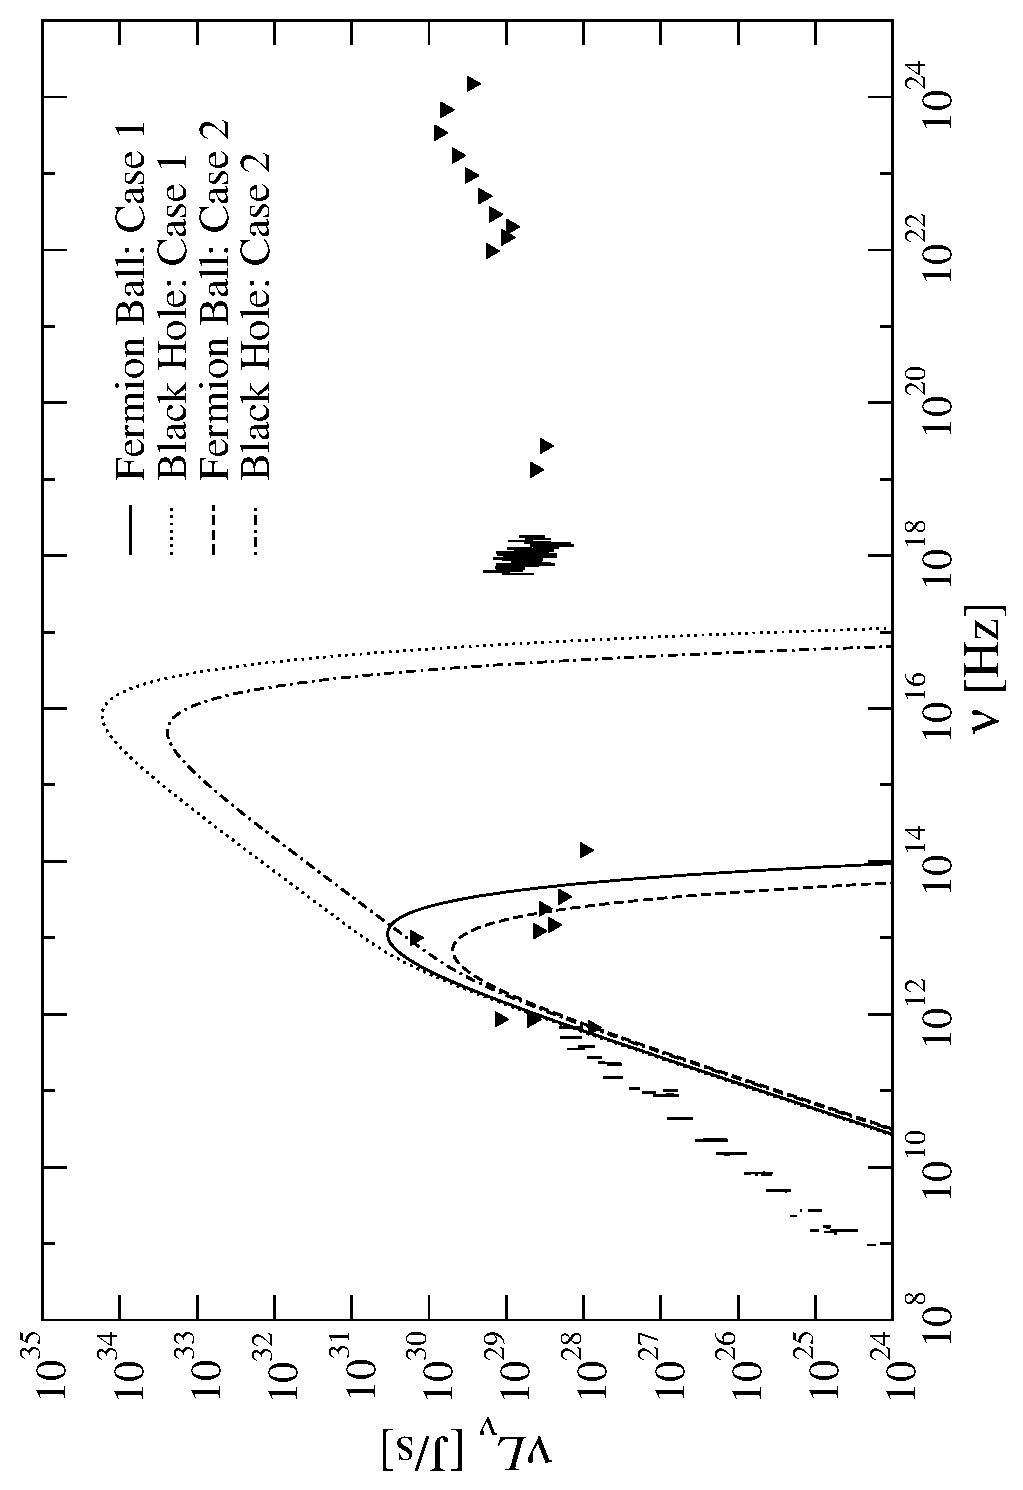
\includegraphics[angle=-90,width=0.9\textwidth]{eps/spectrum-melialimits.eps}
	\caption{The spectrum of the galactic centre due to accretion of gas. ``Case 1'' scenarios have $\dot{M}$=2.948
	$\times 10^{-3}M_\odot$/yr whereas ``Case 2'' scenarios have $\dot{M}$=4.228$\times 10^{-4}M_\odot$/yr.
	Triangular data points are upper limits.}
	\label{fig_accretionspectrummelia}
	\end{center}
\end{figure}

Although the fit from the fermion ball scenario is itself far from perfect, Figure \ref{fig_accretionspectrummelia} clearly shows
that the sudden cut-off in the spectrum around $10^{13}$Hz can indeed be explained by an extended source, and this is the
phenomenon in which we are concerned. The cut-off is due to shearing forces tending to zero at the centre of the fermion ball.
The cut-off can also be explained for the black hole case by using a much lower mass accretion rate.
Unfortunately this will have the consequence that luminosities (at frequencies lower than the cut-off value) are too low. Figure
\ref{fig_accretionspectrumblackholem} displays the spectrum for various mass accretion rates onto a black hole, and Figure
\ref{fig_accretionspectrumfermionballm} the same for the fermion ball scenario.

\begin{figure}[p]
	\begin{center}
	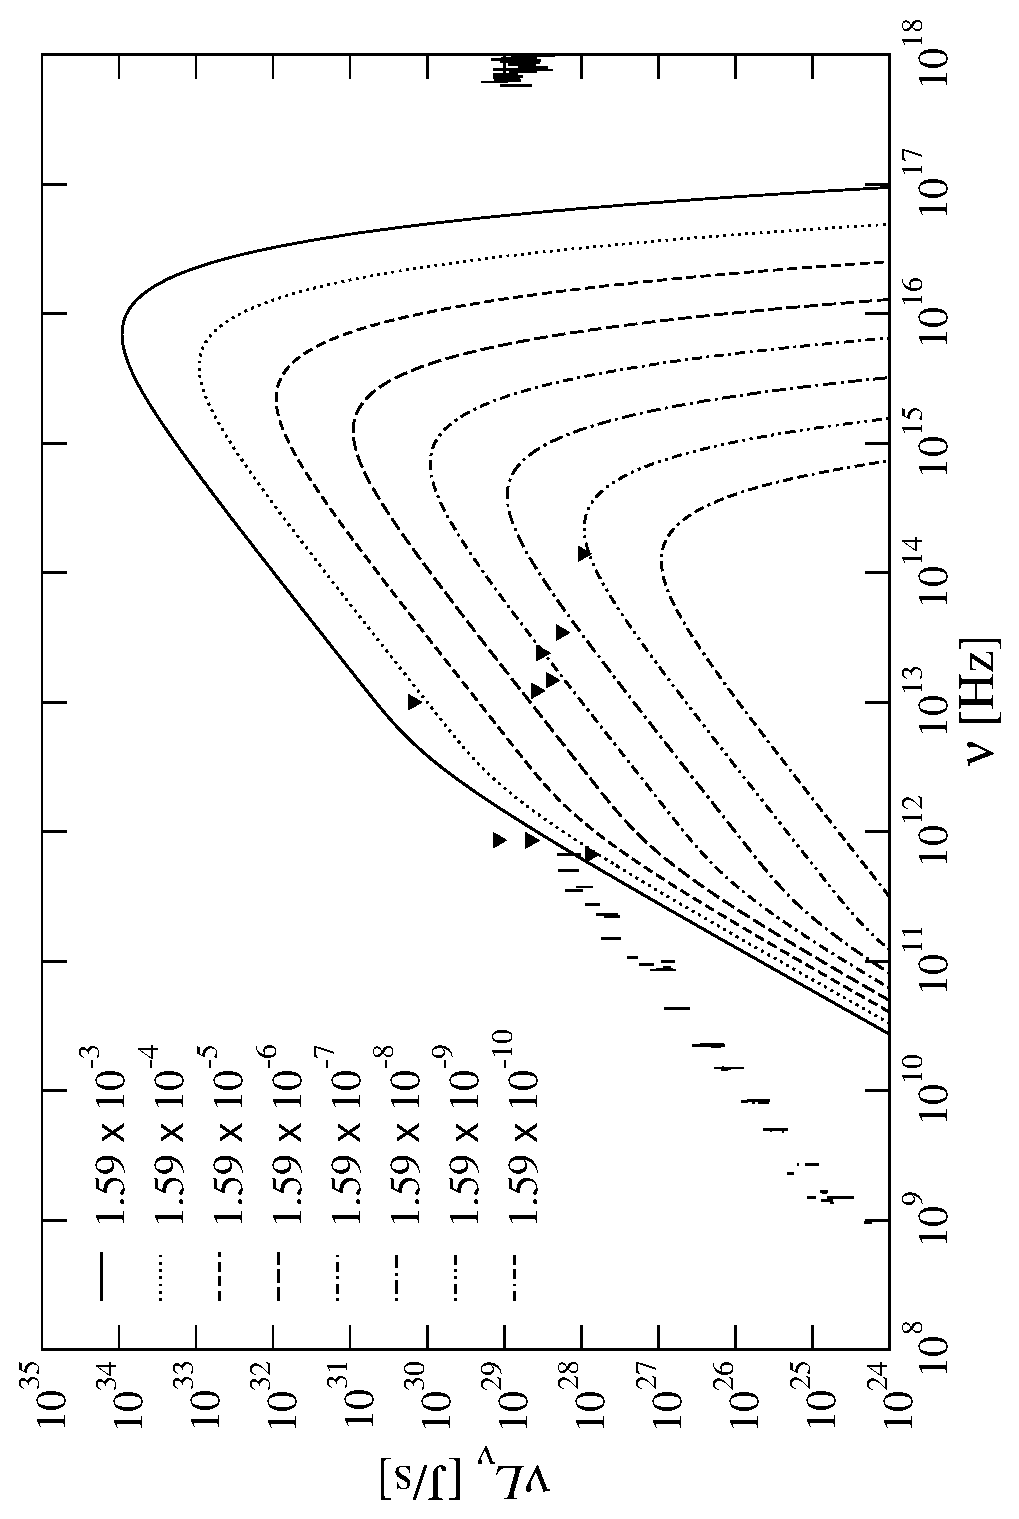
\includegraphics[angle=-90,width=0.9\textwidth]{eps/spectrum-BH-lotsofmdot.eps}
	\caption{The spectrum of the galactic centre due to accretion of gas onto a black hole. Various mass accretion rates are shown in
	units of $M_\odot$/yr.}
	\label{fig_accretionspectrumblackholem}
	\end{center}
\end{figure}
\begin{figure}[p]
	\begin{center}
	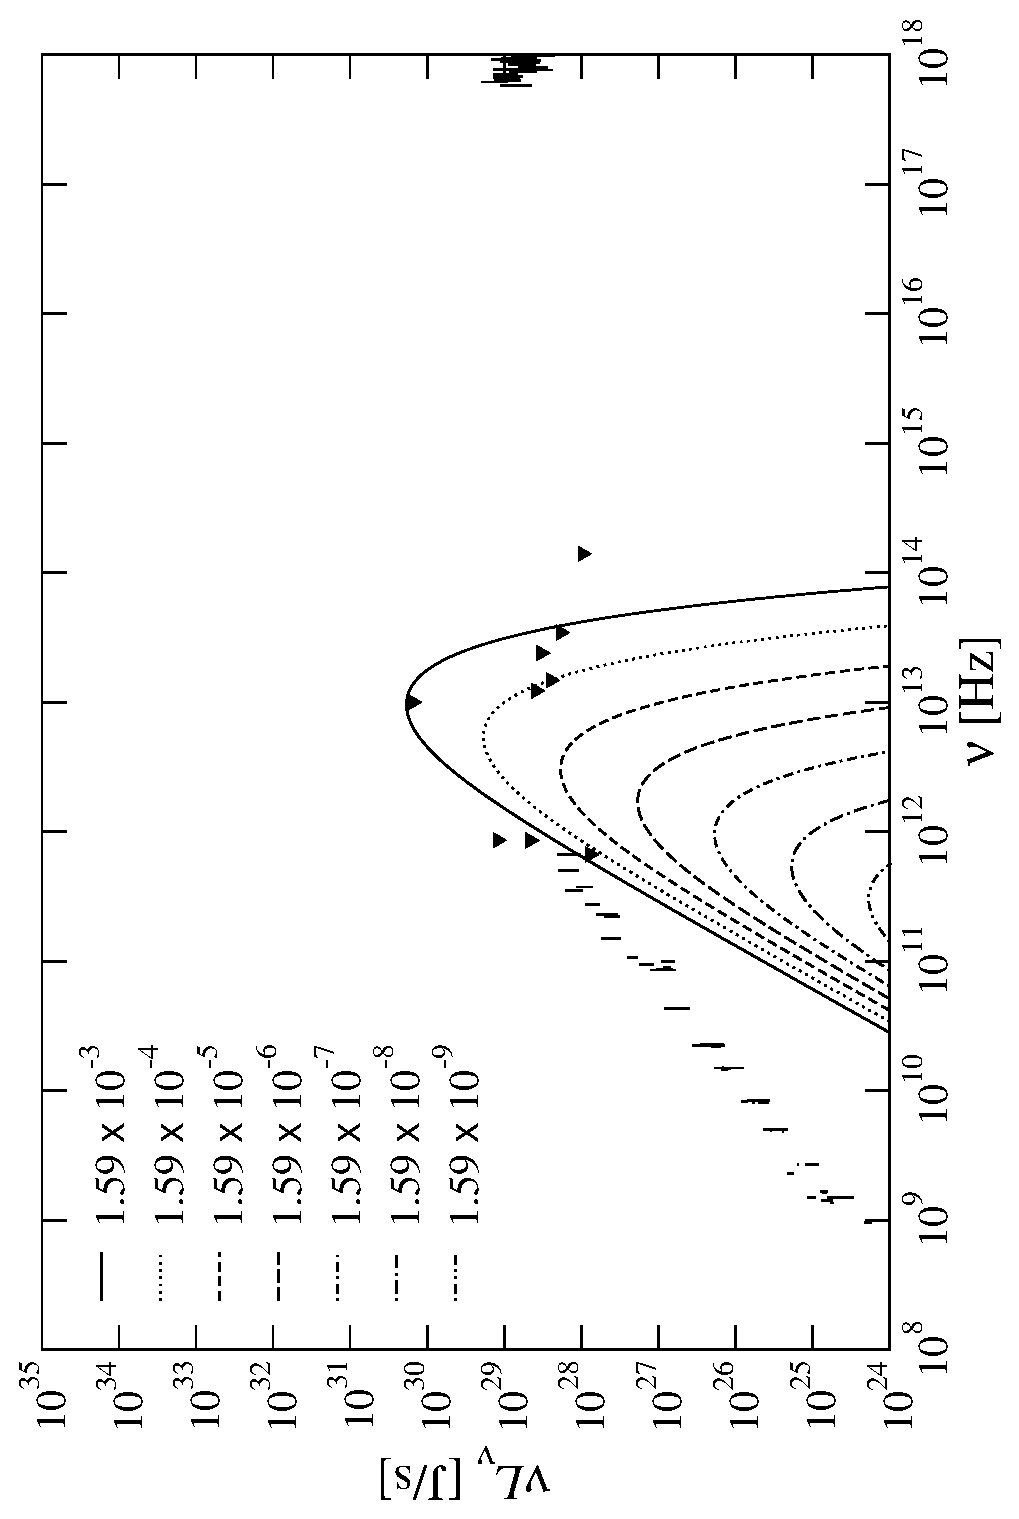
\includegraphics[angle=-90,width=0.9\textwidth]{eps/spectrum-FB-lotsofmdot.eps}
	\caption{The spectrum of the galactic centre due to accretion of gas onto a fermion ball. Various mass accretion rates are shown in
	units of $M_\odot$/yr.}
	\label{fig_accretionspectrumfermionballm}
	\end{center}
\end{figure}

\subsubsection{The Radio and Microwave Spectrum}
Although it has been shown that the fermion ball clearly displays the sudden cut-off in the spectrum in the infra-red region, this simple
model does not explain the `shape' of the spectrum in the radio and microwave region $10^{9} \rightarrow 3 \times 10^{11}$Hz.
Upper limits on the size of the radio source are only a few AU \cite{{ref_radioproper}},
meaning that the emission in this region is not at all due to the
overall accretion of matter, but instead is a result of synchrotron radiation (suggested by the polarisation of the detected photons)
in some localised process. This is evidence of a central object and poses a serious problem to the fermion ball scenario.

\subsubsection{Star Birth}
K-band spectra of stars in the Sgr A* cluster \cite{ref_gezari} reveals that the cluster consists of mainly young, late O $\rightarrow$ early B
main sequence stars. The close proximity of the young stars to the galactic centre is an interesting challenge for either star
formation theory or dynamical theory as the high temperatures, pressures, velocity dispersions and magnetic field strengths in the
central molecular zone inhibit star formation. The black hole scenario is affected even more as there are incredible shearing forces closer
to the nucleus. In the fermion ball scenario the potential becomes harmonic at the centre and shearing forces go linearly to zero, practically
vanishing at $\sim$ 0.01pc.
Using an estimate of new stars simply from the mass accretion rate, a new solar mass star should be expected every 10,000 to 100,000 years
in the fermion ball scenario.

%\section{High Energy Spectrum}
\begin{quotation}
	\raggedleft \it
	X-rays will prove to be a hoax! \\
	-- Lord Kelvin
\end{quotation}
It has already been shown that the fermion ball scenario can account for the cut-out in the IR while the black hole scenario in the
standard theory of accretion, cannot.
This is not, by far, the entire observed spectrum from Sgr A. Here we present some of the higher energy spectral data and briefly
discuss the problems and possible solutions for each of our 2 scenarios.

\subsection{X-Ray Spectrum}
Observations of Sgr A \cite{ref_baganoff} have revealed high emissions at X-ray wavelengths, coincident within 0.014 parsecs to the radio
source Sgr A*. This source corresponds to thermal bremsstrahlung emission with temperature $\sim 10^6$K, in agreement with \cite{ref_melia}.
Not only have these observations shown a distinctive quiescent state spectrum originating from the Sgr A* region,
but rapid `flaring' has also been observed. The X-ray luminosity increases by a
factor of 50 during this flaring state, Figure \ref{fig_fredxray} shows this flaring behaviour alongside the quiescent state.
This flaring suggests only one thing, a small compact object. Time variability measurements also suggest the emitting region not be larger
than 1.2 AU. An extended object such as the fermion ball cannot possibly create this sudden increase in luminosity.

\subsubsection{Iron Line or Fermion Decay}
\label{sec_fermiondecay}
There is, however, also a problem with the black hole scenario producing
such a spectrum. In the quiescent state, there is a peak at around 6.4keV. This peak is absent in the flaring state, and therefore suggests
that the flare `fuel' is of different composure. The peak itself corresponds to an emission line of iron K$_\alpha$, which would require a
gaseous temperature of $5\times 10^7$K. If we were to assume a black hole central object, then the only explanation would
be that any flaring is caused by comets, which are by nature water (and thus lacking the iron to produce the peak). This scenario is
statistically very unlikely, as we must be prepared to see flaring from all forms of fuel if the object is indeed a black hole.
\begin{figure}[ht]
	\begin{center}
	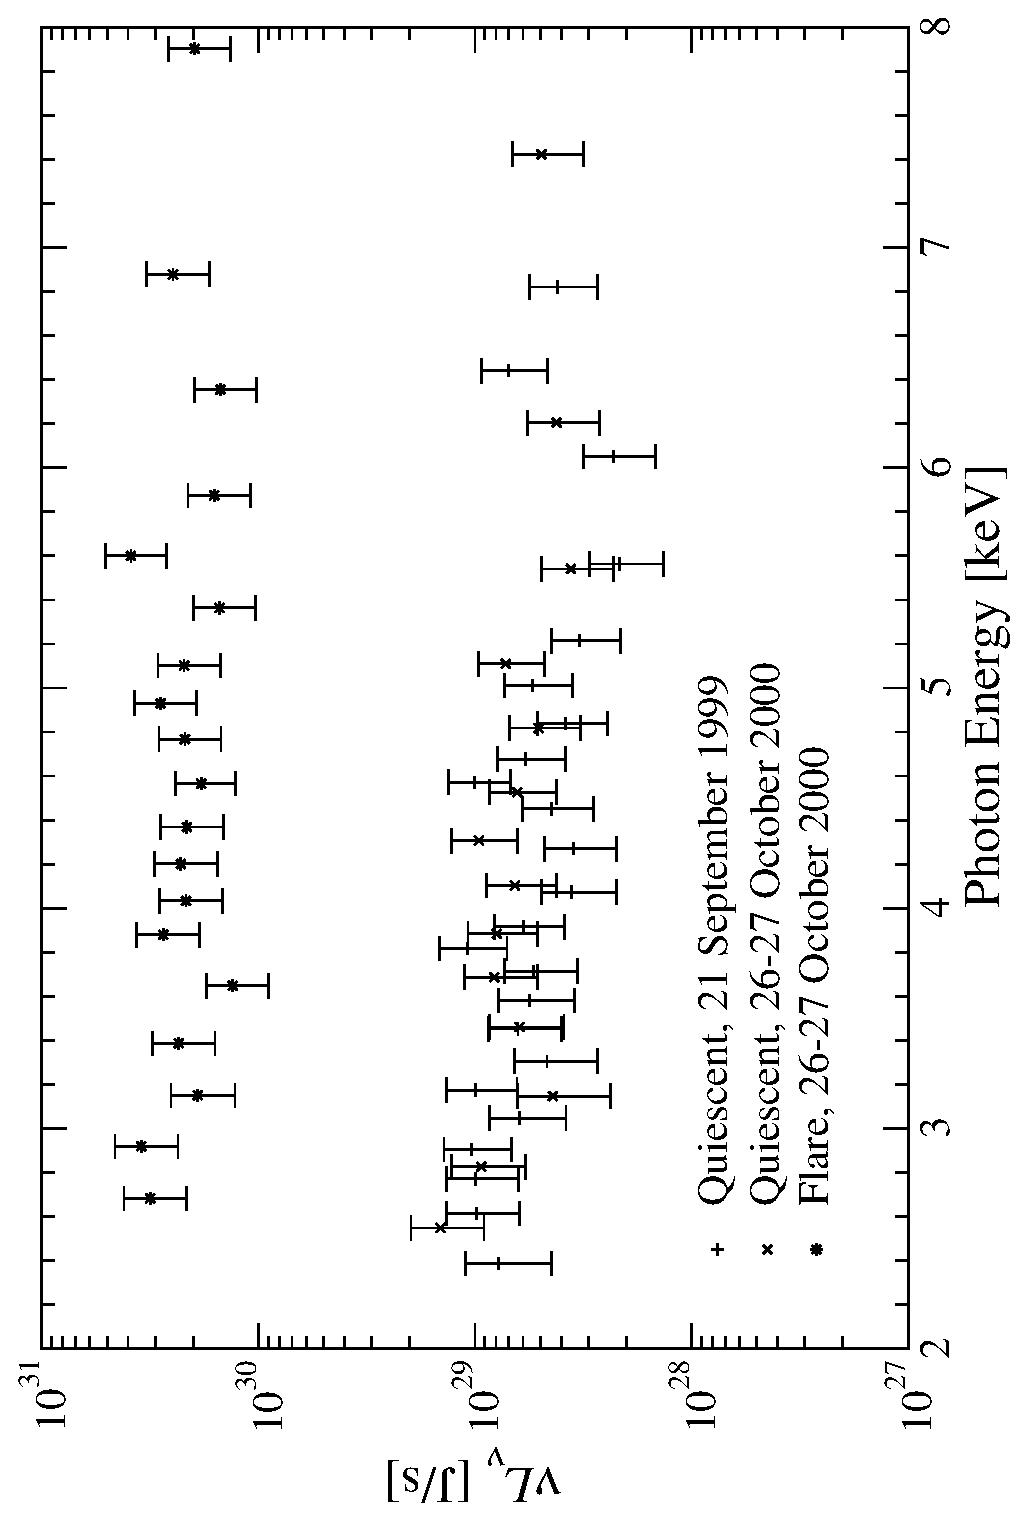
\includegraphics[angle=-90,width=0.9\textwidth]{eps/xray-nulum.eps}
	\caption{X-ray spectrum.}
	\label{fig_fredxray}
	\end{center}
\end{figure}

An alternative solution is to consider the possibility of another compact object in the vicinity of Sgr A*, such as an X-ray binary.
In the
black hole scenario, the binary would need to be between us and Sgr A*, and we would therefore eventually observe the source disappear around
the back of the black hole, but we are still left with the problem of the Fe K$_\alpha$ line. For the fermion ball scenario we place
the binary incident with Sgr A*, but we explain the 6.4keV peak by a completely different process altogether. As the fermion ball is by
nature, made of fermions, we expect them to decay. A Feynman diagram is shown for a possible decay path associated to a sterile neutrino which
results in a nearly massless active neutrino taking away half the energy.
\begin{figure}[!h]
	\begin{center}
	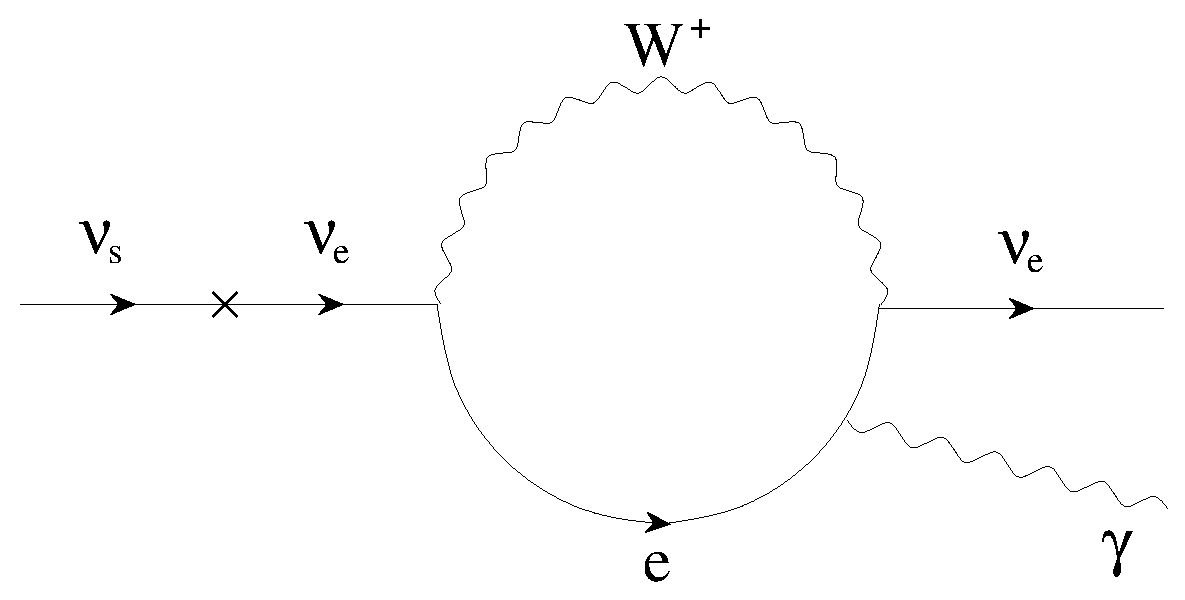
\includegraphics[angle=0,width=0.6\textwidth]{eps/fermiondecay.eps}
	\caption{Feynman diagram for the radiative decay of a sterile neutrino into an active neutrino
	and a photon of energy $\frac{m_{\nu_s}}{2}$.}
	\label{fig_feynmandiag}
	\end{center}
\end{figure}

\noindent
This photon with sharp energy should cause a peak in the spectrum which we may
observe. If we were to speculate that the 6.4keV peak was evidence of this process, we would require a fermion ball containing fermions of
mass 12.8keV. This is obviously too low a value to be consistent with Section \ref{sec_fermionlimits}. However, if the fermions were of the
degeneracy 4 variety, then we would be able to use Equation (\ref{eqn_classicalfermiondegeneracyrelation}) to say that the fermion ball would
display the same mass distribution with $g$=4, $m_\nu$=12.8keV as with $g$=2, $m_\nu$=15.2keV. We have already shown that 16keV
fermions display properties capable of explaining orbital motion of cluster stars and the IR cut-out, it is also quite possible to
show the same for 15.2keV fermions. Considering errors in the peak measurement, fermions of up to $g$=4, $m_\nu$=13.5keV,
equivalent to $g$=2, $m_\nu$=16keV would also produce such a spectral line.

Another advantage of the X-ray binary presence is that we would have a possible source for the synchrotron emission which explains the
radio and microwave spectrum, missing from the accretion model.

However, due to the constant influx of fast moving stars through the galactic centre, we should expect an X-ray binary resident
at the centre to be ejected after a short period of time. This X-ray binary phenomenon could therefore be a short term effect.

\subsubsection{On Possible Measurement of $z$ and $v_z$ for Nearby Stars}
\label{sec_zandvz}
The photons from the X-ray flare will be incident upon stars near the galactic centre, including S0-1, S0-2 and S0-4. As the
resolution of X-ray maps is not enough to see a reflection from these stars directly, we may look at the IR spectra
and possibly observe corresponding activity, initiated by the X-ray flare. By measuring the time delay between the X-ray
flare (assumed to be from Sgr A*) and IR activity at a neighbouring star, we may calculate $z$ for that star.

It may also be that such a flare would intensify well known spectral lines, allowing for a corresponding measurement of $v_z$.
Such a measurement would instantly discern between black hole or extended source models of the galactic centre, by
using the phase space analysis presented in Section \ref{sec_futureps}.
We now show how such a time delay measurement would lead to a value of $z$, Figure \ref{fig_geomfindzvz}.
\begin{figure}[!h]
	\begin{center}
	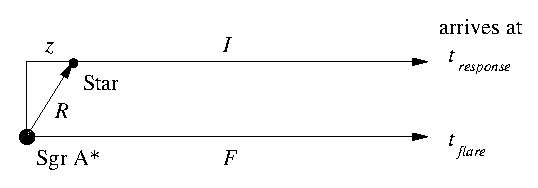
\includegraphics[angle=0,width=0.7\textwidth]{eps/zmeasure.eps}
	\caption{Geometry of the photons from the X-ray flare and response.}
	\label{fig_geomfindzvz}
	\end{center}
\end{figure}

\noindent
We measure $\Delta t=t_{{\rm {\it response}}}-t_{{\rm {\it flare}}}$. The distances $F$ and $I$ in terms of the incident times are
$F=ct_{{\rm {\it flare}}}$ and $I+R=ct_{{\rm {\it response}}}$ where $c$ is the speed of light. It is clear that $I=F-z$, giving us
a suitable form of equations which we may solve for $z$, giving
\begin{equation}
	z=\frac{\left(x^2+y^2\right)}{2c\Delta t} -\frac{c\Delta t}{2}
\end{equation}

\subsection{$\gamma$-Ray Spectrum}
Although it has been mentioned that there is a $\gamma$-ray spectrum associated with the galactic centre \cite{ref_gamma}, it is however
only spatially resolved to within a radius of 0.2 degrees from Sgr A*. Since we are dealing with objects already constrained within 0.5
arcsec, the $\gamma$-ray spectrum cannot conclusively be associated with Sgr A*, except as an upper limit.

\section{Fermion Halo and Dark Matter in the Galaxy}
\begin{quotation}
	\raggedleft \it I believe there are
	15,747,724,136,275,002,577,605,653,961,181,555,468,044,\\
	717,914,527,116,709,366,231,425,076,185,631,031,296 \\
	protons in the universe and the same number of electrons.\\
	-- Sir Arthur Eddington
\end{quotation}
An extension of the fermion ball theory is to consider fermions with finite temperature \cite{ref_finitetemp}.
Such an extension results in a fermion halo around
the central ball already investigated in this thesis. In this section, we briefly discuss how the finite temperature extension leads to a
halo structure and the effect this has upon the dark matter problem in our galaxy \cite{ref_halo}.

\subsection{Dark Matter Within Our Galaxy}
It is well known, from the rotation curves of an increasing number of galaxies, that there are substantial amounts of dark matter in the halos
of galaxies. Typically, dark matter contributes about 10 times more mass than the ordinary matter which is contained in visible stars, dust
and gas. It is worthwhile to speculate that the super-massive compact dark objects at the galactic centres may have something to do with the
dark matter in the halos.

In the case of the Milky Way, this dark matter is arranged in a nearly spherically symmetric halo, stretching roughly a third the distance to
the Andromeda galaxy in radial component. There are a number of indications from nucleosynthesis \cite{ref_halonucleo},
micro-lensing \cite{ref_halomicrolens}, structure formation and microwave background data \cite{ref_halocmbstruct},
which indicates at least part of this dark matter halo cannot be made of ordinary matter. In the following, we will be primarily
concerned with this non-baryonic dark matter which does not interact efficiently with ordinary matter and radiation, except gravitationally.

Cold dark matter scenarios provide an excellent description of the formation of the large-scale structure in the universe. However, they fail
on galactic and sub-galactic scales \cite{ref_halofailcdm} because the absence of velocity dispersion causes the dark matter to sink
to the centre.
These problems can be bypassed by the introduction of warm dark matter \cite{ref_halofailwdmgalacticform},
and postulating the existence of a sterile neutrino \cite{ref_sterileneutrino}. The creation of the desired amount of sterile neutrino
dark matter in the early universe, with
about $\Omega_{\nu_s}=0.3$ of the critical density today, can be achieved for a sterile neutrino of mass 16keV with a mixing angle $\theta$
given by $\sin^2 2\theta \sim 10^{-12}$, see Figure \ref{fig_sterileelectronphase}.
The angle $\theta$ describes the mixing of a sterile neutrino with an active neutrino, Equation (\ref{eqn_sterileneutrino}), and therefore
makes the dark matter particle observable through its radiative decay into an active neutrino and a photon, with a lifetime of about
$\tau \sim 10^{20}$years. See Figure \ref{fig_feynmandiag}.
\begin{figure}[pt]
	\begin{center}
	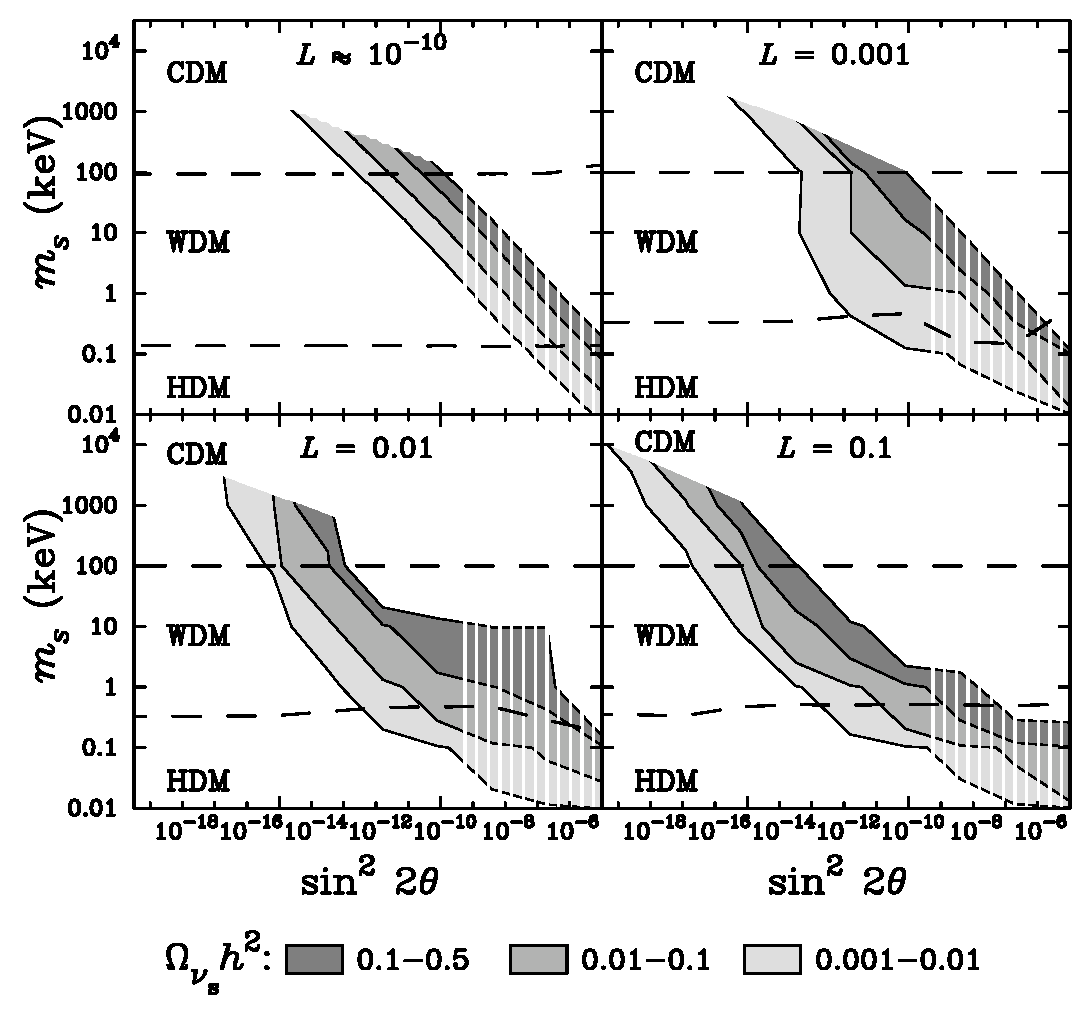
\includegraphics[width=0.9\textwidth]{eps/omegaepanel.eps}
	\caption{Regions of $\Omega_{\nu_s}$ produced by resonant and non-resonant electron neutrino mixing with a sterile neutrino.
	$L$ denotes lepton asymmetry. Regions of parameter space disfavoured by supernova core collapse considerations are shown
	with vertical stripes. From \cite{ref_sterileneutrino}.}
	\label{fig_sterileelectronphase}
	\end{center}
\end{figure}
\begin{figure}[pb]
	\begin{center}
	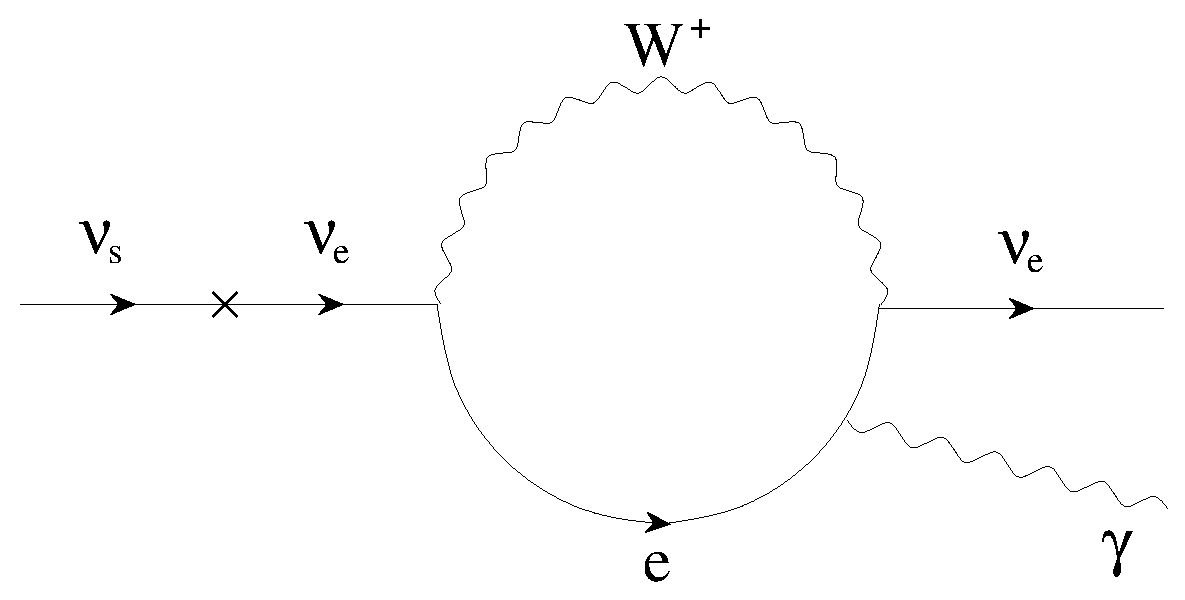
\includegraphics[angle=0,width=0.6\textwidth]{eps/fermiondecay.eps}
	\caption{Feynman diagram for the radiative decay of a sterile neutrino into an active neutrino
	and a photon of energy $\frac{m_{\nu_s}}{2}$.}
	\label{fig_feynmandiag}
	\end{center}
\end{figure}

\subsection{The Fermion Halo}
It has been shown that a non-relativistic self interacting fermion gas may undergo a first order gravitational
phase transition, from a diffuse state to a condensed state \cite{ref_halo2,ref_halo3,ref_halo4}.
Within a Fermi gas, self energy from gravity is balancing with thermal energy. If the gravity dominates, we have a condensed state,
whereas if the thermal energy dominates, we have a diffuse state. The temperature at which the fermions are close to the point of
gravitational collapse is called the critical temperature and is where the phase transition occurs. A simple analytical model has been
proposed by \cite{ref_chavanis}, agreeing quite well with the numerical simulations.

We now briefly discuss the non-relativistic Thomas-Fermi theory for a self gravitating gas of $N$ fermions with mass $m_\nu$ at a
temperature $T$ enclosed in a sphere of radius $R$. For large $N$ we can assume the fermions move in a spherically symmetric mean-field
potential $\phi(r)$ which satisfies Poisson's equations
\begin{eqnarray}
	\frac{d\phi}{dr} &=& \frac{GN}{r^2}
	\label{eqn_halo1} \\
	\frac{dM(r)}{dr} &=& 4\pi r^2 m n
	\label{eqn_halo2}
\end{eqnarray}
The number density ($n$) is determined by the Fermi-Dirac distribution (units $\hbar=c=k=1$)
\begin{equation}
	n=\frac{\rho}{m_\nu}=g_\nu \int \frac{d^3q}{(2\pi)^3} \left[ 1+e^{\left(\frac{q^2}{2 m_\nu T} + \frac{m_\nu \phi}{T}
	- \frac{\mu}{T}\right)}\right]^{-1}
	\label{eqn_halo3}
\end{equation}
For each solution $\phi(r)$ of (\ref{eqn_halo1}), the chemical potential $\mu$ is adjusted so that the constraint
\begin{equation}
	\int^R_0 dr 4\pi r^2 n(r) = N
	\label{eqn_halo4}
\end{equation}
is satisfied. Equations (\ref{eqn_halo2}) and (\ref{eqn_halo3}) are integrated using the boundary conditions
\begin{equation}
	\phi(0)=\phi_0 \qquad \qquad M(0)=0
	\label{eqn_halobounds}
\end{equation}
It is useful to introduce the degeneracy parameter
\begin{equation}
	\eta = \frac{\mu}{T} - \frac{m_\nu \phi}{T}
	\label{eqn_halo5}
\end{equation}
with the strongest degeneracy $\eta_0$ obtained at the centre, fixed by the condition $M(R)=m_\nu N$, where $R$ is the outer boundary.
Outside of $R$, we have the usual $\propto \frac{1}{r}$ Newtonian potential.
Equations (\ref{eqn_halo2}), (\ref{eqn_halo4}) and (\ref{eqn_halo3}) define the gravitational Thomas-Fermi equation, which is solved numerically.

One first solves (\ref{eqn_halo2}) to yield $M(R)$ as a function of $\eta_0$, leaving 3 free parameters:
$N$, $T$ and $R$. $N$ is fixed by setting the fermion mass and using an appropriate total mass consistent with observation.
We make the simple calculation $N=\frac{M}{m_\nu}$.

In \cite{ref_halo}, the values $m_\nu=15$keV, $M=2 \times 10^{12} M_\odot$, $R=200$kpc and $T=3.75 \times 10^{-3}$K were used.
The radius limit is based upon the estimated size of the galaxy halo. The
temperature is estimated as a result of violent relaxation \cite{ref_haloviolentrelax}, and is thus
directly related to the gravitational plus thermal energy.

The solution is a fermion ball (as investigated in this thesis) alongside a low density halo, extending out to the radius $R$.

\subsection{Rotation Curve of Our Galaxy}
Using the numerical mass distribution of the halo, the rotation curve for objects within our galaxy may be calculated. The bulge
and disk must also be included for comparison to data. The total rotation curve for our galaxy is shown
in Figure \ref{fig_halorotation}. The bulge is modelled as a spherically symmetric matter distribution \cite{ref_halobulge} in the form
\begin{equation}
	\rho_b(s)=\frac{e^{-hs}}{2s^3} \int^\infty_0 du \frac{e^{-hsu}}{\left[ (u+1)^8 -1\right]^{\frac{1}{2}}}
	\label{eqn_halobulge}
\end{equation}
where $s=\left( \frac{r}{r_0} \right)^{\frac{1}{4}}$, $r_0$ is the effective radius of the bulge. We adopt values such that
$M_b=1.5\times 10^{10}M_\odot$ \cite{ref_halobulgevalues}.
The contribution of the disk's circular velocity component is modelled as \cite{ref_halodisk}
\begin{equation}
	\Theta_d(r)^2=\Theta_d(r_0)^2\frac{1.97 \left( \frac{r}{r_0}\right)^{1.22}}{\left[\left( \frac{r}{r_0}\right)^2 +0.78^2 \right]^{1.43}}
	\label{eqn_halodisk}
\end{equation}
where we take $r_0=13.5$kpc and $\Theta_d(r_0)=100$km/s. We assume (for simplicity) that the disk does not influence the mass distribution of
either the bulge or the halo.
\begin{figure}[t]
	\begin{center}
	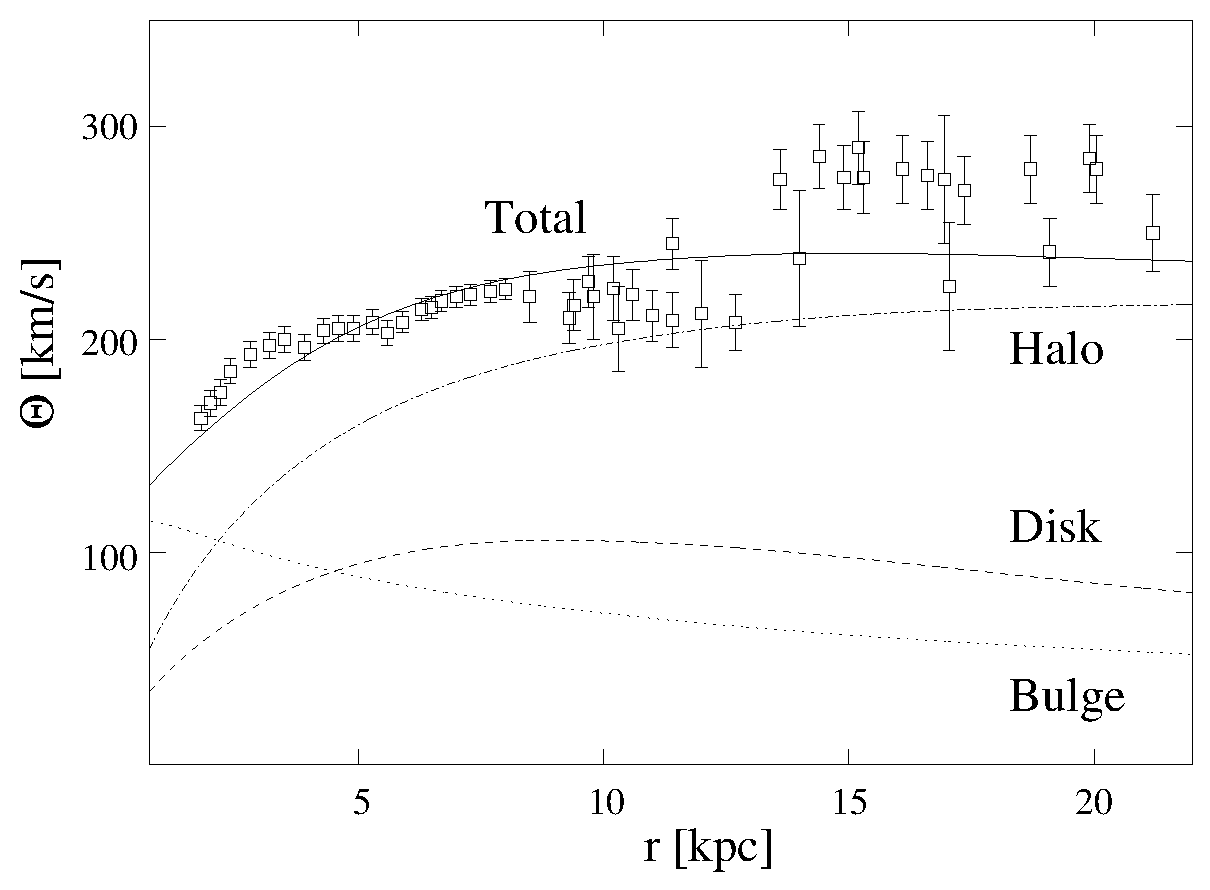
\includegraphics[width=0.9\textwidth]{eps/halo.eps}
	\caption{Fit to the Galactic rotation curve. Data points are from \cite{ref_halodata} and the graph itself is from \cite{ref_halo}.}
	\label{fig_halorotation}
	\end{center}
\end{figure}

The rotation curve clearly shows that the standard disk and bulge models, in combination with the halo theory, describe reasonably the circular
velocity distribution within our galaxy to just beyond a distance of 20kpc. We conclude that the fermion halo sufficiently describes the dark
matter distribution within our own galaxy.

In summary, the Thomas-Fermi theory applied to finite temperature, self gravitating, fermionic gas yields a mass distribution
explaining the dark matter distribution within the Milky Way halo, whilst also producing a fermion ball at the centre. This theory therefore
allows that the fermions in the halo are the same as those at the galactic centre, Sgr A*.

\chapter{Conclusions}
\label{conclusion}

In this thesis, we have studied symmetric and non-symmetric (twisted) D-branes
of the six dimensional Nappi-Witten spacetime and discovered that the majority
of the noncommutative geometries are simpler than one would have expected; the
symmetric branes all observe a flat space with zero NS flux, allowing standard
open string models to be used to calculate the noncommutativity parameter. We
found a class of commutative null branes and a class of noncommutative Euclidean
D3-branes, analogous to branes in a constant magnetic field.

Central to the discoveries of the noncommutative nature of branes in $\NW_6$ was
the ability to perform Penrose-G\"uven limits on embedded spaces and keep track
of the supergravity fields in isometric embedding diagrams. To achieve this, we
produced formal coordinate free restrictions that one must observe in order to
be guaranteed a commuting diagram.

The most interesting non-symmetric branes were found to be Hpp-waves
\textit{without} the characteristic Nappi-Witten NS flux, and hence classified
as Cahen-Wallach spacetimes, not Nappi-Witten spacetimes as previously thought.
One of these non-symmetric branes was found to possess a complicated worldvolume
flux that corresponds to an electric field and hence does not exhibit a well
defined decoupling of the massive string states. However, by choosing an
appropriate gauge for the $\NW_6$ $B$ field, we have been able to discover a
spatially varying noncommutativity, analogous to that of the Dolan-Nappi model.
This gauge choice results in non-vanishing Poisson brackets that reproduce the
Nappi-Witten Lie algebra in the small time limit.

Inspired by this noncommutative geometry that reproduces the Nappi-Witten Lie
algebra, we proceeded to obtain closed and explicit forms of the
$\star$-products for several physically important orderings; corresponding to
the global and Brinkman coordinatisations of the spacetime and the Weyl
symmetric ordering. By using the formalism of generalised Weyl systems, we were
able to calculate the Hopf algebra of twisted isometries.

By placing linear constraints on the $\star$-derivatives, we restricted our
analysis to the flat space limit; the trade off being that we were able to
obtain Leibniz rules for the derivatives and therefore proceed in a systematic
manner. After formalising the rules for integration we advanced to the scalar
field theory, confirming that our analysis is consistent with a flat space
limit. We document the pseudo-orthonormal frames and twisted derivatives that
deform the commutative Laplacian, finding that only transverse space motion is
effected by the commutativity.

Restricting the algebraic analysis of the Nappi-Witten Lie algebra to embedded
worldvolumes, we confirmed the previous analysis of the noncommutative
geometries and developed a method that allows a more systematic construction of
the deformed worldvolume field theories of generic D-branes in $\NW_6$ in the
semi-classical regime.

All techniques throughout this thesis have been presented in such a manner that
they may be applied to a broad range of homogeneous pp-waves supported by a
constant Neveu-Schwarz flux.

Further research in this area could involve the study of an interacting $\Phi^4$
theory. In canonical noncommutative field theory, we calculate products such as
$e^{iq_ix^i}\star e^{iq_i'x^i}$ at each vertex in a Feynman diagram. We now know
that such an exponential product will be spacetime-dependent, meaning that
planar Feynman diagrams will be granted a phase shift analogous to those
observed in non-planar quantum field theories (such that result in UV/IR
mixing). We must also face the possibility of violations in energy and momentum
conservation.

%%% Local Variables: 
%%% mode: latex
%%% TeX-master: "main.tex"
%%% End: 

\appendix
\section{Reduction of Terms in \ref{sec_fermionballtempdist}}
\label{app_solnoffermiontempdist}
Equation (\ref{eqn_fbeffectivetemp}) contains the problem in $x$ and $\mu(x)$
\begin{eqnarray*}
	x\sqrt{\frac{\mu(x)}{x^3}}\frac{d}{dx}\sqrt{\frac{\mu(x)}{x^3}}
\end{eqnarray*}
using
\begin{eqnarray*}
	\frac{d}{dx}\left(\frac{u}{v}\right) = \frac{v\dot{u}-u\dot{v}}{v^2} \\
	\frac{d}{dx}\left(u^n\right) = nu^{n-1}\dot{u}
\end{eqnarray*}
where we assign
\begin{eqnarray*}
	\begin{array}{ll}
	u=\mu(x)^{\frac{1}{2}} & v=x^{\frac{3}{2}} \\
	\dot{u}=\frac{1}{2}\mu^{-\frac{1}{2}}\mu '(x)\qquad\quad & \dot{v}=\frac{3}{2}x^{\frac{1}{2}} 
	\end{array}
\end{eqnarray*}
it follows that
\begin{eqnarray*}
	\frac{d}{dx}\left(\frac{\mu(x)}{x^3}\right)^{\frac{1}{2}}
	&=&\frac{\sqrt{x}}{2}\frac{x\mu(x)^{-\frac{1}{2}}\mu '(x)-3\mu(x)^{\frac{1}{2}}}{x^3} \\
	&\times& x\sqrt{\frac{\mu(x)}{x^3}} = \frac{1}{2}\frac{x\mu '(x)-3\mu(x)}{x^3}
\end{eqnarray*}
so that we can make the reduction
\begin{eqnarray*}
	x\sqrt{\frac{\mu(x)}{x^3}}\frac{d}{dx}\sqrt{\frac{\mu(x)}{x^3}} = \frac{1}{2}\frac{x\mu '(x)-3\mu(x)}{x^3}
\end{eqnarray*}

\section{Radiation Processes}
\label{app_opticallythickapprox}
An (unpolarised) radiation field is defined by the {\it specific intensity} ($I_\nu$), which gives the flux of energy per second per unit area
per solid angle per unit frequency interval
\begin{eqnarray*}
	dE=I_\nu dA \cos\theta d\nu d\Omega dt
\end{eqnarray*}
The {\it radiation flux} ($F_\nu$) is the rate at which energy crosses a unit area independent of direction and is obtained by integrating
over a solid angle
\begin{eqnarray*}
	F_\nu=\int I_\nu \cos\theta d\Omega
\end{eqnarray*}
The {\it specific luminosity} ($L_\nu$) of a source is the flux integrated over an area enclosing the source
\begin{eqnarray*}
	L_\nu = \int F_\nu dA
\end{eqnarray*}
the variation of $I_\nu$ in a medium which is emitting and absorbing is given by the {\it radiative transfer equation} which simply expresses
energy conservation for the radiation field. In the time independent case in a direction ${\bf n}$
\begin{eqnarray*}
	{\bf n}\cdot \nabla I_\nu = -\mu_\nu I_\nu + j_\nu
\end{eqnarray*}
where $\mu_\nu$ is the absorption coefficient and $j_\nu$ the emission coefficient, effectively the properties and state of the medium. It is
customary to characterise the medium by the {\it source function} ($S_\nu$)
\begin{eqnarray*}
	S_\nu = \frac{j_\nu}{\mu_\nu}
\end{eqnarray*}
The {\it optical depth} ($\tau_\nu$) along a path from source to observer is defined by
\begin{eqnarray*}
	d\tau_\nu=\mu_\nu ds
\end{eqnarray*}
Giving total specific intensity over an optical depth
\begin{eqnarray*}
	\frac{dI_\nu}{d\tau_\nu} = -I_\nu + S_\nu
\end{eqnarray*}
If the radiation field corresponds to thermal equilibrium at a temperature $T$, we know that $I_\nu=B_\nu(T)$, the black body spectrum.
Irrespective of the radiation mechanism, we can relate
\begin{eqnarray*}
	S_\nu=B_\nu(T)=\frac{2h\nu^3}{c^2\left(e^{\frac{h\nu}{kT}}-1\right)}
\end{eqnarray*}
If the medium can be characterised by a temperature $T$ (i.e. thermal emission) then we have Kirchhoff's law, independent of whether the
radiation field is Planckian.
\begin{eqnarray*}
	S_\nu = \frac{j_\nu}{\mu_\nu} = B_\nu(T)
\end{eqnarray*}
In general the source function is determined by the state populations in the medium. A necessary condition for a thermal radiation spectrum
is that the optical depth $\tau_\nu \rightarrow \infty$. In this case we say that the medium is {\it optically thick}, which in general,
means that $I_\nu=S_\nu$. On the other hand if $\tau_\nu \rightarrow 0$ we can neglect absorption and we get
\begin{eqnarray*}
	I_\nu=\int j_\nu ds
\end{eqnarray*}
Such a medium is said to be {\it optically thin}. Returning to the optically thick case, once we have a source function, we make the
following relations (as explained) to give us the observables $F_\nu$ or $L_\nu$, depending upon the preference of the experimentalist.
\begin{eqnarray*}
	I_\nu &=& S_\nu = \frac{2h\nu^3}{c^2\left(e^{\frac{h\nu}{KT}}-1\right)} \\
	F_\nu &=& \frac{4\pi h \nu^3\cos{i}}{c^2D^2} \int\frac{R}{e^{\frac{h\nu}{KT}}-1}dR \\
	L_\nu &=& 4\pi D^2 F_\nu = \frac{16\pi^2 h \nu^3\cos{i}}{c^2} \int\frac{R}{e^{\frac{h\nu}{KT}}-1}dR
\end{eqnarray*}

In the text, we have assumed an optically thick medium so that we may simply use a black body as our radiative mechanism. The absorption
coefficient is $\mu_\nu \propto \kappa \rho$, which decreases for a low density gas, and thus optical depth decreases.
$\kappa$ is the opacity, and is calculated from the radiative transfer equation
\begin{eqnarray*}
	\kappa(\nu ,T)=\frac{c^2}{8\pi \nu^2}A_{21}\frac{g_2}{g_1}n_1\left[1-e^{\frac{h\nu_0}{kT}}\right]\phi(\nu)
\end{eqnarray*}
As temperatures are generally low in the fermion ball case, the gas will not be ionised and therefore $\kappa$ will also aid in
decreasing the optical depth. The gas density is low under both scenarios.

This goes to show that an optically thin approximation may be more appropriate for the fermion ball scenario.
In an optically thin accretion disk, a different radiative mechanism must be used as the black body approximation is
no longer appropriate, such a valid mechanism could be a thermal bremsstrahlung spectrum.

\section{Numerical Techniques}
The numerical problems in this thesis are Ordinary Differential Equations (ODE's). The first step to solve such a problem is to reduce
the system to a series of first order differentials. e.g. for the Lan\'e-Emden Equation (\ref{eqn_laneemden})
\begin{eqnarray*}
	\frac{d^2v(x)}{dx^2} = -\frac{v(x)^\frac{3}{2}}{x^\frac{1}{2}}
\end{eqnarray*}
we may write as two, first order equations
\begin{eqnarray*}
	z = \frac{dv}{dx} \qquad \qquad \frac{dz}{dx} = -\frac{v^\frac{3}{2}}{x^\frac{1}{2}}
\end{eqnarray*}
The simplest way to solve such an equation is to use Euler's method ($f$ is the known derivative of a function, with specified parameters)
\begin{eqnarray*}
	b_{n+1}=b_n + h f\left(a_n, b_n\right)
\end{eqnarray*}
which advances a solution from $a_n$ to $a_{n+1} \equiv a_n + h$. It advances the solution through an interval $h$, but uses derivative
information only at the beginning of that interval, meaning the error is only one power of $h$ lower than the correction $O(h^2)$.
e.g. In the Lan\'e-Emden example, if we solve with a numerical step size of $10^{-2}$, then the error in each value will be
$(10^{-2})^2=10^{-4}$ of the correction, which is rather high. Small step sizes must be used for accuracy, but this results in
incredibly long run times of programs.

Another technique is the Runge-Kutta method, which takes a `trial' step to the midpoint of the interval, then uses the value of both $a$
and $b$ at that midpoint to compute a more accurate step across the whole interval.
\begin{eqnarray*}
	k_1 &=& h f\left(a_n, b_n\right) \\
	k_2 &=& h f\left(a_n + \frac{1}{2}h, b_n + \frac{1}{2} k_1\right) \\
	b_{n+1} &=& b_n + k_2 + O\left(h^3\right)
\end{eqnarray*}
This is a third order Runge-Kutta as the error is of that order. In this thesis, a fourth order Runge-Kutta was employed in mass
distribution solutions, with a step size of $10^{-6}$, giving an error of $10^{-24}$ times the correction for each step.

All code was written in C and is available\footnote{http://neutrino.phy.uct.ac.za} under the GNU Public Licence, requiring the
GNU Science Library\footnote{http://sources.redhat.com/gsl} for compilation.

\begin{thebibliography}{100}
	\bibitem{ref_centralobjects}			L. C. Ho, J. Kormendy,
								{\it astro-ph/0003267; astro-ph/0003268}
	\bibitem{ref_centralobjectsbiggest}		F. Macchetto, A. Marconi, D. J. Axon, A. Capetti, W. Sparks, P. Crane,
								{\it ApJ} {\bf 489} (1997) 579
	\bibitem{ref_ghezmotion}			A. M. Ghez, B. L. Klein, M. Morris, E. E. Becklin,
								{\it ApJ} {\bf 509} (1998) 678
	\bibitem{ref_radioproper}			D. C. Backer, R. A. Sramek,
								{\it ApJ} {\bf 524} (1999) 805
	\bibitem{ref_vlba}				G. C. Bower, D. C. Backer,
								{\it ApJL} {\bf 496} (1998) 97
	\bibitem{ref_kundt}				W. Kundt,
								{\it Ap\&SS} {\bf 172} (1990) 109
	\bibitem{ref_radiopic}				T. N. Larosa, N. E. Kassim, T. J. Lazio, S. D. Hyman,
								{\it AJ} {\bf 119} (2000) 207
	\bibitem{ref_baganoffsubmit}			F. K. Baganoff {\it et al.},
								{\it astro-ph/0102151}
	\bibitem{ref_maoz}				E. Maoz,
								{\it ApJL} {\bf 494} (1998) 181
	\bibitem{ref_whitehole}				G. Burbidge, F. Hoyle,
								{\it ASP Conf. Ser.} {\bf 102} The Galactic Center
	\bibitem{ref_fermion1}				R. D. Viollier, D. Trautmann, G. B. Tupper,
								{\it Phys. Lett. B} {\bf 306} (1993) 79
	\bibitem{ref_fermion2}				N. Bili\'{c}, D. Tsiklauri, R. D. Viollier,
								{\it Prog. Part. Nucl. Phys.} {\bf 40} (1998) 17
	\bibitem{ref_fermion3}				D. Tsiklauri, R. D. Viollier,
								{\it Astropart. Phys.} {\bf 12} (1999) 199
	\bibitem{ref_thomasfermiapproach}		R. D. Viollier,
								{\it Prog. Part. Nucl. Phys.} {\bf 32} (1994) 51
	\bibitem{ref_bilic}				N. Bili\'{c}, F. Munyaneza, R. D. Viollier,
								{\it Phys. Rev. D} {\bf 59} (1998) 024003
	\bibitem{ref_classicalapproach}			F. Munyaneza, D. Tsiklauri, R. D. Viollier,
								{\it ApJ} {\bf 526} (1999) 744\\
							F. Munyaneza, R. D. Viollier,
								{\it ApJ} {\bf 564} (2002) 274
	\bibitem{ref_bosonstar}				D. F. Torres, S. Capozziello, G. Lambiase,
								{\it Phys. Rev. D} {\bf 62} (2000) 104012
	\bibitem{ref_neutrinostar}			M. A. Markov,
								{\it Phys. Lett.} {\bf 10} (1964) 122
	\bibitem{ref_neutrinomass}			J. Bonn {\it et al.},
								{\it Nucl. Phys. B.} {\bf 91} (2001) 273
	\bibitem{ref_neutrinomass2}			Y. Fukuda {\it et al.} (Super-Kamiokande Collaboration),
								{\it Phys. Rev. Lett.} {\bf 81} (1998) 1562
	\bibitem{ref_4neutrinos}			D. E. Groom {\it et al.},
								{\it Eur. Phys. J. C} {\bf 15} (2000) 1
	\bibitem{ref_neutralino}			V. S. Berezinsky, A. V. Gurevich, K. P Zybin,
								{\it Phys. Lett. B} {\bf 294} (1992) 221
	\bibitem{ref_nonneutrino}			E. W. Kolb, M. S. Turner,
								{\it The Early Universe}, Addison-Wesley (1989)
	\bibitem{ref_sterileneutrino1}			X. Shi, G. M. Fuller,
								{\it Phys. Rev. Lett.} {\bf 82} (1999) 2832
	\bibitem{ref_sterileneutrino}			K. Abazajian, G. M. Fuller, M. Patel
								{\it Phys. Rev. D} {\bf 64} (2001) 023501
	\bibitem{ref_gravitino}				D. H. Lyth,
								{\it Phys. Lett. B} {\bf 488} (2000) 417
	\bibitem{ref_axinomass}				K. Tamvakis, D. Wyler,
								{\it Phys. Lett. B} {\bf 112} (1982) 451
	\bibitem{ref_axino}				T. Goto, M. Yamaguchi,
								{\it Phys. Lett. B} {\bf 276} (1992) 103
	\bibitem{ref_axinodark}				L. Covi, H. B. Kim, J. E. Kim, L. Roszkowski,
								{\it J. High Energy Phys.} {\bf 0105} (2001) 033
	\bibitem{ref_sterileneutrinoconstraint1}	G. M. Fuller, R. A. Malaney,
								{\it Phys. Rev. D} {\bf 43} (1991) 3136
	\bibitem{ref_sterileneutrinoconstraint2}	E. W. Kolb, M. S. Turner,
								{\it Phys. Rev. Lett.} {\bf 67} (1991) 5
	\bibitem{ref_sterileneutrinoanalytic}		S. Dodelson, L. M. Widrow,
								{\it Phys. Rev. Lett.} {\bf 72} (1994) 17
	\bibitem{ref_gravitinothermal}			S. Sarkar,
								{\it Rep. Prog. Phys.} {\bf 59} (1996) 1493
	\bibitem{ref_gravitinononthermal}		D. H. Lyth, D. Roberts, M. Smith,
								{\it Phys. Rev. D} {\bf 57} (1998) 7120
	\bibitem{ref_formation}				N. Bili\'{c}, R. Lindebaum, G. B. Tupper, R. D. Viollier,
								{\it Phys. Lett. B} {\bf 515} (2001) 105
	\bibitem{ref_bosonform}				M. Colpi, S. Shapiro, I. Wasserman,
								{\it Phys. Rev. Lett.} {\bf 57} (1986) 20
	\bibitem{ref_bosonformtf}			A. S. Parkins, D. F. Walls,
								{\it Phys. Rep.} {\bf 303} (1998) 1
	\bibitem{ref_ghezorbits}			A. M. Ghez, M. Morris, E. E. Becklin, A. Tanner, T. Kremenek,
								{\it Nature} {\bf 407} (2000) 349
	\bibitem{ref_eckartorbits}			A. Eckart, R. Genzel, T. Ott, R. Sch\"{o}del,
								{\it MNRAS} {\bf 331} (2002) 917
	\bibitem{ref_thomasfermi}			L. H. Thomas,
								{\it Proc. Cambridge Phil. Soc.} {\bf 23} (1924) 542\\
							E. Fermi,
								{\it Zeit. Phys.} {\bf 48} (1928) 73
	\bibitem{ref_majoranasolution}			S. Esposito,
								{\it physics/0111167}
	\bibitem{ref_tolmanpaper}			R. C. Tolman,
								{\it Phys. Rev.} {\bf 55} (1939) 364
	\bibitem{ref_tolmanbook}			R. C. Tolman,
								{\it Relativity, Thermodynamics and Cosmology}, Oxford (1934)
	\bibitem{ref_oppenheimervolkoff}		J. R. Oppenheimer, G. M. Volkoff,
								{\it Phys. Rev.} {\bf 55} (1939) 374
	\bibitem{ref_chandra}				S. Chandrasekhar,
								{\it Stellar Structure}, University of Chicago Press (1939)
	\bibitem{ref_meliareview}			F. Melia, H. Falcke,
								{\it Annu. Rev. Astron. Astophys.} {\bf 39} (2001) 309
	\bibitem{ref_FKR}				J. Frank, A. King, D. Raine,
								{\it Accretion Power in Astrophysics}, Cambridge (1992)
	\bibitem{ref_yusefmorris}			F. Yusef-Zadeh, M. Morris,
								{\it ApJL} {\bf 371} (1991) 59
	\bibitem{ref_rees}				M. J. Rees,
								{\it In the Galactic Centre}, New York:AIP (1982)
	\bibitem{ref_narayan}				Narayan {\it et al},
								{\it ApJ} {\bf 492} (1998) 554
	\bibitem{ref_melia}				F. Melia,
								{\it ApJL} {\bf 387} (1992) 25
	\bibitem{ref_cokerthesis}			R. Coker,
								{\it PhD Thesis}, University of Arizona (1999)
	\bibitem{ref_gezari}				S. Gezari, A. M. Ghez, E. E. Becklin, J. Larkin, I. S. McLean, M. Morris,
								{\it astro-ph/0205186}
%	\bibitem{ref_baganoff}				F. K. Baganoff,
%								{\it et al. Nature}, {\bf 413} (2001) 45
%	\bibitem{ref_gamma}				H. A. Mayer-Hasselwander,
%								{\it et al. Astron. Astrophys.} {\bf 335} (1998) 161
	\bibitem{ref_finitetemp}			N. Bili\'{c}, R. D. Viollier,
								{\it Phys. Lett. B} {\bf 408} (1997) 75
	\bibitem{ref_halo}				N. Bili\'{c}, G. B. Tupper, R. D. Viollier,
								{\it astro-ph/0111366}
	\bibitem{ref_halonucleo}			H. Kurki-Suonio, E. Sihvola,
								{\it Phys. Rev. D} {\bf 63} (2001) 083508
	\bibitem{ref_halomicrolens}			K. Griest,
								{\it et al. astro-ph/9506016}
	\bibitem{ref_halocmbstruct}			X. Chen, S. Hannestad, R. J. Scherrer,
								{\it Phys. Rev. D} {\bf 65} (2002) 123515
	\bibitem{ref_halofailcdm}			A. Tasitsiomi,
								{\it astro-ph/0205464}
	\bibitem{ref_halofailwdmgalacticform}		Y. P. Jing,
								{\it Mod. Phys. Lett. A} {\bf 16} (2001) 1795
	\bibitem{ref_halo2}				N. Bili\'{c}, R. D. Viollier,
								{\it Phys. Lett. B} {\bf 408} (1997) 75
	\bibitem{ref_halo3}				N. Bili\'{c}, R. D. Viollier,
								{\it Gen. Rel. Grav.} {\bf 31} (1999) 1105
	\bibitem{ref_halo4}				N. Bili\'{c}, R. D. Viollier,
								{\it Eur. Phys. J. C} {\bf 11} (1999) 173
	\bibitem{ref_chavanis}				P-H. Chavanis,
								{\it Phys. Rev. E} {\bf 65} (2002) 056123
	\bibitem{ref_haloviolentrelax}			D. Lynden-Bell,
								{\it MNRAS} {\bf 136} (1967) 101
	\bibitem{ref_halobulge}				G. de Vaucouleurs, W. D. Pence,
								{\it ApJ} {\bf 83} (1978) 1163
	\bibitem{ref_halobulgevalues}			P. D. Sackett,
								{\it ApJ} {\bf 483} (1997) 103
	\bibitem{ref_halodisk}				M. Persic, P. Salucci, F. Stell,
								{\it MNRAS} {\bf 281} (1986) 27
	\bibitem{ref_halodata}				R. P. Olling, M. R. Merrifield,
								{\it MNRAS} {\bf 311} (2000) 361
\end{thebibliography}

\clearpage
\pagestyle{empty}
{\bf {\Large \noindent Acknowledgements}}
\\$\big.$\\ \noindent
Firstly I would like to thank my supervisor, Prof. R. D. Viollier, for this
interesting topic and the funding I needed to survive. Thanks go to Dr. G.
Tupper for help on the Newtonian derivations and to Prof. A. Ghez, Dr. F.
Baganoff and Dr. R. Coker for their communal spirit in the sharing of their
data. Physics needs more people with your attitude, in my opinion `read it from
the graph!' is a line spoken by frauds and ASCII is always welcome!

I must thank the UCT funding and housing departments for much amusement they
have given me in their amazing ability to be incompetent in every way possible.
My thanks for zero funding and an overpriced shanty.

Credit must be given to the GNU community, whom collectively have created an
operating system which has allowed me to run the simulations and produce in a
professional manner, this thesis and the figures therein. Thanks to Wayne Kerr
for many enlightening discussions on the numerics.

Thanks to the entire staff of the UCT physics department, you made me feel very
welcome! I would also like to thank the great friends I have made in the time I
have spent in this beautiful country. Hopefully we can all have a pint on my
turf next time!

I am very grateful to my parents, without their support this adventure would not
have been possible. Same goes for the big man upstairs, who is always looking
out for me.

\clearpage

\end{document}
